\documentclass[10pt, a4paper]{article}

\usepackage[top=3.5cm, left=3.5cm, right=3.0cm, bottom=3.0cm, includehead, includefoot]{geometry}%margem 
\usepackage[]{graphicx} 
\usepackage{amssymb,amsmath}
%\usepackage[brazilian]{babel}
\usepackage[utf8]{inputenc}
\usepackage[square, numbers, comma, sort&compress]{natbib}
\usepackage{microtype}
\usepackage{siunitx}
\usepackage{cite}%bibliografia
%\usepackage{indentfirst} %espaço primeiro parágrafo
\setlength{\parindent}{0em} %parágrafo 1,25cm
\setlength{\parskip}{0.5\baselineskip}

\usepackage{caption}
\usepackage{float} %posicionar figuras
\usepackage[font=scriptsize]{caption}
\usepackage[font=scriptsize]{subcaption} %legenda de figuras

\DeclareMathSizes{5}{5}{5}{5}

\usepackage{subcaption}
\usepackage{booktabs}
\usepackage{fixltx2e} 
\usepackage{multirow}
\usepackage{array}
\usepackage{adjustbox}
\usepackage{wrapfig}
%\usepackage{breqn}
\usepackage{color}

\usepackage{rotating}

\usepackage{fancyhdr}
\pagestyle{fancy}
\rfoot{\copyright Nasser Alkmim}
\lfoot{2014}
\lhead{\leftmark}
\rhead{\thepage}
\cfoot{}
\renewcommand{\headrulewidth}{0pt}
\renewcommand{\footrulewidth}{0pt}

\usepackage{multicol}

\usepackage{psfrag}
\usepackage[pdfstartview=FitH,backref,colorlinks,bookmarksopen,urlcolor=black,linkcolor=black]{hyperref}


\font\ursymbol=psyr at 9pt % You also use other font sizes.
\def\urpartial{\mbox{\ursymbol\char"B6}}

%\usepackage{titlesec}
%\titlespacing{\section}{0cm}{.5cm}{.5cm}
%\titlespacing{\subsection}{0cm}{.5cm}{.5cm}
%\titlespacing{\subsubsection}{0cm}{.5cm}{.5cm}

%\numberwithin{equation}{section} 

\usepackage{chngcntr}

%\counterwithin{figure}{section}

%\usepackage{empheq}
%\newcommand*\widefbox[1]{\fbox{\hspace{2em}#1\hspace{2em}}}

\usepackage{tikz}
\usetikzlibrary{shapes,arrows}
\tikzstyle{block} = [rectangle, draw, 
    text width=5em, text centered, rounded corners, minimum height=2em]
\tikzstyle{line} = [draw, -latex']


\begin{document}

\title {

\includegraphics[scale=.3]{fig/logo7.eps} \\
% \textbf{{\Huge \texttt{elf}}}LAB}
}
\author{Nasser Alkmim}
\date{ {\footnotesize\today}}
\maketitle

\begin{abstract}

\end{abstract}

\tableofcontents

\thispagestyle{empty}
\clearpage
\pagestyle{fancy}


\section{Heat Equation}

From conservation of energy, the variation of thermal energy through time must be equal to the net flux of heat through the boundaries through time. Jean-Baptiste Joseph Fourier, French mathematician, in 1822 published his work on heat flow under the title \emph{Théorie analytique de la chaleur}.

\subsection{Fourier's Law}

The local heat flux density is given by,
\begin{equation}
\phi_i = - \kappa \theta_{,i} \mathbf{\hat{e}}_i,
\end{equation}
where, $\kappa$ is the thermal conductivity and $ \theta_{,i}$ is the gradient of the temperature. The subscript $i$ indicates the number of dimensions. The vectors in an orthonormal basis of the Cartesian system can be represented by $\{ \mathbf{\hat{e}}_i\}$. Physically the equation means that the flux density is proportional to the negative of the temperature gradient, the negative sign indicates that a positive flux represents an increase in temperature. With this we can define on each point and at each time the local flux density.

\subsection{Newton's Law of Cooling}

The change on internal local thermal energy $\Delta q$ is related to the change on internal temperature $\Delta \theta$ by:
\begin{equation}
\Delta Q =c \rho \Delta \theta
\end{equation}
where $c$ is the specific heat and $\rho$ the density.

\subsection{Conservation of Energy}

Focusing on a general infinitesimal element, the energy balance must occur, which means that the change in the energy content of the element is due the net energy flux through its boundaries. The \emph{local} net heat flux is given by the divergent of the flux density.
\begin{equation}
 (\phi_i)_{,i} + \dfrac{\Delta Q}{\Delta t}  = 0
\end{equation}
instantaneously, 
\begin{align*}
&\dfrac{\partial Q}{\partial t} = - (\phi_i)_{,i}  \\
& c  \rho \dfrac{\partial \theta}{\partial t} = \kappa \theta_{,ii} \\
& \dfrac{\partial \theta}{\partial t} =  k \theta_{,ii} + q,
\end{align*}
where, $q$ is an extra internal source of energy and $k=\frac{\kappa}{c \rho}$ is the thermal diffusivity. The diffusivity measures the property of the material to conduct heat, energy. The bigger its value means the energy will spread easily and the changes in the temperature are going to be smaller. The units for this property is watts per meter kelvin.

\section{Steady Heat Equation}

\subsection{Model}

The equation to be solved for $\theta(x_i)$ on the domain $\Omega$,
	\begin{equation}
	k \theta_{,ii} + q = 0 , \qquad x_i \in \Omega,
	\end{equation}
where,
\begin{align*}
\theta_{,ii} &= \dfrac{\urpartial ^2 \theta}{\urpartial  x_1^2} + \dfrac{\urpartial ^2 \theta}{\urpartial  x_2^2}\\
&= \theta_{,x_1x_1} + \theta_{,x_2x_2} .
\end{align*}
This equation is obtained through conservation of energy and the constitutive law, Fourier's equation. Physically, we have the divergent of the energy equation, i.e., flux of energy through the boundaries, plus an internal source of energy, $q = q(x_i, t)$, must be equal to the time change of energy. This case the time change is considered to be equal zero, steady state case.

\subsection{Weak Form}

The weak form of the steady state heat equation which is a form of Poisson's equation is
\begin{align*}
&\int_{\Omega} v \; \left(k \theta_{,ii} + q \right) \, \mathrm{d}\Omega = 0\\
& \int_{\Omega} v \;  k \theta_{,ii} \, \mathrm{d}\Omega + \int_{\Omega}  v\; q  \, \mathrm{d}\Omega  =  0 \\
& \int_{\Omega} k  (v\theta_{,i})_{,i} \; \mathrm{d}\Omega - \int_{\Omega}k v_{,i} \theta_{,i}  \; \mathrm{d}\Omega +  \int_{\Omega}  v\; q  \, \mathrm{d}\Omega =  0 \\
& \int_{\Omega} v_{,i}k \theta_{,i}  \; \mathrm{d}\Omega    -
 \int_{\Omega}  v\; q  \, \mathrm{d}\Omega - 
 \int_{\urpartial \Omega} k  v\theta_{,i}\; \mathrm{d}\Gamma = 0.
\end{align*}


\subsubsection{Green's Theorem}

The Green's Theorem is expressed as
\begin{align*}
&\nabla \cdot (v \nabla \theta ) = v \left( \nabla \cdot \nabla \theta \right) + \nabla v \cdot \nabla \theta \\
&(v \theta_{,i})_{,i} = v \theta_{,ii} + v_{,i} \theta_{,i}.
\end{align*}


\subsection{Finite Elements Approximation}

The following approximation is considered for each element,
\begin{align*}
\tilde{\theta}^e &= \phi_n a_n^e, \qquad n=1,2,3,4;\\
&= \sum_{n=1}^4 \phi_i a_i^e.
\end{align*}
The test function $v$ is also approximated with the same shape functions (Galerkin's approach):
\begin{align*}
\tilde{v}^e &= \phi_m b_m^e, \qquad m=1,2,3,4;\\
&= \sum_{m=1}^4 \phi_m b_m^e.
\end{align*}

\subsubsection{Shape Functions}

The shape functions on the isoparametric space defined with the axes $(\xi_1, \xi_2)$ are:
\begin{align*}
\phi_1 = \frac{1}{4} (1 - \xi_1)(1 - \xi_2); \\
\phi_2 = \frac{1}{4} (1 + \xi_1)(1 - \xi_2); \\
\phi_3 = \frac{1}{4} (1 + \xi_1)(1 + \xi_2) ;\\
\phi_4 = \frac{1}{4} (1 - \xi_1)(1 + \xi_2) .\\
\end{align*}

\subsection{Approximate Solution on the Weak Form}

Subdividing the domain between the elements, $e$, the equation becomes:
\begin{multline*}
\sum_e 
 \int_{\Omega^e} \left( \sum_{m=1}^4 \phi_{m,i} b_m^e \right) k \left( \sum_{n=1}^4 \phi_{n,i} a_n^e \right)\, \mathrm{d}\Omega^e -
\int_{\Omega^e} \left( \sum_{m=1}^4 \phi_{m} b_m^e \right) q \, \mathrm{d}\Omega^e - \\
\int_{\urpartial \Omega^e} \left( \sum_{m=1}^4 \phi_{m} b_m^e \right) k \theta_{,i} \, \mathrm{d}\Gamma^e =0 .
\end{multline*}
Removing the index for the elements, the equation can be solved for each individual element:
\begin{multline*}
 \int_{\Omega} \left( \sum_{m=1}^4 \phi_{m,i} b_m \right) k \left( \sum_{n=1}^4 \phi_{n,i} a_n \right)\, \mathrm{d}\Omega - 
\int_{\Omega} \left( \sum_{m=1}^4 \phi_{m} b_m \right) q \, \mathrm{d}\Omega -
\int_{\urpartial \Omega} \left( \sum_{m=1}^4 \phi_{m} b_m \right) k \theta_{,i} \, \mathrm{d}\Gamma =0 .
\end{multline*}
In matrix form, the equation can be rewritten
\begin{align*}
&\boldsymbol{b} \mathbf{K} \boldsymbol{a} -\boldsymbol{b} \mathbf{R} = 0 ;\\
&\mathbf{K} \boldsymbol{a}- \mathbf{R} = 0,
\end{align*}
where each element will have a stiffness matrix $\mathbf{K}$ and a load matrix $\mathbf{R}$. Because the elements share some of their boundaries the assemblage of the individual matrices into a global one will require special attention, the algorithm uses the connective matrix in order to build the assembled matrix. The components of the stiffness matrix are,
\begin{align*}
K_{mn} =  \int_{\Omega} \phi_{m,i} k \phi_{n,i}  \, \mathrm{d}\Omega , \qquad m,n=1,2,3,4.
\end{align*}
Each element will have its set of four shape functions $\phi_i$ and those are going to be evaluated on each element sub-domain. The load vector components,
\begin{align*}
R_{m} =  \int_{\Omega} \phi_{m}q \, \mathrm{d}\Omega + \int_{\urpartial \Omega} \phi_m \; k \theta_{,i}\, \mathrm{d}\Gamma , \qquad m=1,2,3,4.
\end{align*}
The load is divided in two parts, the first is due the internal heat source and the second, at the boundaries, due the heat flux source (Neumann condition).

\section{Transient Heat Equation}

\subsection{Partial Differential Equation}

The transient form of the heat equation with internal heat source is:

\begin{equation}
k \theta_{,ii} + q = \dfrac{\partial \theta}{\partial t} , \qquad x_i \in \Omega
\end{equation}



\subsection{Weak Form}

\begin{align*}
&\nabla \cdot (k \nabla \theta)  + q = \dfrac{\partial \theta}{\partial t} \\ 
& \int_\Omega v \nabla \cdot (k \nabla \theta) \; \mathrm{d}\Omega + \int_\Omega v q\; \mathrm{d}\Omega = \int_\Omega v \; \dfrac{\partial \theta}{\partial t}\; \mathrm{d}\Omega \\
&\int_{\partial \Omega} \nabla \cdot (v \; k \nabla \theta) \; \mathrm{d}\Gamma - \int_\Omega \nabla v \cdot k\nabla \theta \; \mathrm{d}\Omega +  \int_\Omega v q\; \mathrm{d}\Omega = \int_\Omega v \;\dfrac{\partial \theta}{\partial t}\; \mathrm{d}\Omega \\
&\int_\Omega v \; \dfrac{\partial \theta}{\partial t}\; \mathrm{d}\Omega + \int_\Omega \nabla v \cdot k\nabla \theta \; \mathrm{d}\Omega = \int_\Omega v q\; \mathrm{d}\Omega + \int_{\partial \Omega} \nabla \cdot (v \; k \nabla \theta) \; \mathrm{d}\Gamma
\end{align*}


\subsection{Finite Elements Approximation}

Para cada elemento, tem-se a seguinte aproximação:
\begin{align*}
\tilde{\theta}^e &= \phi_n a_n^e, \qquad n=1,2,3,4\\
&= \sum_{n=1}^4 \phi_i a_i^e
\end{align*}

e usando a mesma funções para aproximar a função teste $v$:
\begin{align*}
\tilde{v}^e &= \phi_m b_m^e, \qquad m=1,2,3,4\\
&= \sum_{m=1}^4 \phi_m b_m^e
\end{align*}

\subsection{Approximate Solution on the Weak Form}

The extra term with the time derivative is a square matrix the same size as the stiffness, number of degrees of freedom.

\begin{equation*}
\mathbf{M \dot{a} +  K a = R}
\end{equation*}

where,

\begin{equation*}
M_{mn} = \int_\Omega \phi_m \phi_n \; \mathrm{d}\Omega, \qquad m,n = 1,2,3,4
\end{equation*}



\subsection{Time Discretization with Finite Differences}

\begin{align*}
\mathbf{M} \left( \dfrac{\mathbf{a}(t+\Delta t) - \mathbf{a}(t)}{\Delta t}\right) + \mathbf{Ka}(t)  =\mathbf{R} \\
\mathbf{M} \mathbf{a}(t+\Delta t) = \Delta t (\mathbf{R} - \mathbf{Ka}(t)) + \mathbf{Ma}(t)
\end{align*}



\section{Implementation}

The implementation process consists in create a series of classes, methods and functions for each step of the calculation. Starting with the mesh with its geometry, attributes and properties. The elements with its stiffness matrix, mass matrix and load vector. A function for applying the boundary condition and lastly a set of other functions for post processing the results.


The element class will be responsible to produce elemental matrices, the core of the calculations are made here. In order to solve the integrals in a efficient manner we need a numerical approach. Gaussian quadrature (GQ) is the most adequate method. The GQ works very nicely with the mapping scheme to the isoparametric domain. Therefore, the integrals require a change of variables, a Jacobian computation and a summation over the GQ points.


The way the algorithm work is the following: A loop over each element in order to create matrices and vectors for each of them and a loop over the 4 GQ points. At each GQ points, each entry will be calculated and assigned to a variable. For each GQ point, a series of methods are called within the mesh object

\subsection{Preliminaries}
\subsubsection{Mapping}

The mapping $(x_i) \rightarrow (\xi_j)$ is given by,
\begin{equation*}
x_i = G(\xi_j) = x_i(\xi_j), \qquad i,j = 1,2
\end{equation*}
one reads $x_i$ as a function of $\xi_j$. The shape function's gradient as a function of the natural coordinates is
\begin{align*}
\phi_{,i} &= \dfrac{\urpartial \phi}{\urpartial x_i} \\
	&= \left( \dfrac{\urpartial \phi}{\urpartial x_1}, \dfrac{\urpartial \phi}{\urpartial x_2} \right)\\
	&= \left( \dfrac{\urpartial \phi(x_i)}{\urpartial x_1}, \dfrac{\urpartial \phi (x_i)}{\urpartial x_2} \right)\\
	&= \left( \dfrac{\urpartial \phi(x_i(\xi_j))}{\urpartial x_1}, \dfrac{\urpartial \phi (x_i(\xi_j))}{\urpartial x_2} \right) \\
	&= \left( \dfrac{\urpartial \phi(\xi_j)}{\urpartial x_1}, \dfrac{\urpartial \phi (\xi_j)}{\urpartial x_2} \right) \\
	&= \left( \dfrac{\urpartial \phi(\xi_j)}{\urpartial \xi_1} \dfrac{\urpartial \xi_1}{\urpartial x_1} + \dfrac{\urpartial \phi(\xi_j)}{\urpartial \xi_2} \dfrac{\urpartial \xi_2}{\urpartial x_1},  \dfrac{\urpartial \phi(\xi_j)}{\urpartial \xi_1} \dfrac{\urpartial \xi_1}{\urpartial x_2} + \dfrac{\urpartial \phi(\xi_j)}{\urpartial \xi_2} \dfrac{\urpartial \xi_2}{\urpartial x_2}\right) \\
	&= \phi(\xi_j)_{,u} \xi_{u,i} .
\end{align*}
The subscript (${}_{,i}$) indicates the spatial derivative with relation to Cartesian coordinates and the subscript (${}_{,u}$) the spatial derivative with respect to the \emph{natural coordinates} on the isoparametric domain. The gradient is calculated first with respect to the Cartesian coordinates and then, using the chain rule, with the natural coordinates. 

The way this gradient is implemented is based on the storage of the individual shape functions, its derivatives with respect to $\xi_1$ and $\xi_2$ and using the Jacobian matrix in order to find $\frac{\partial \xi_u}{\partial x_i}$. All the storage is done with the Gauss points so we avoid excessive functions evaluations.

In matrix form we treat this gradient as 
\begin{equation*}
\phi_{,i} = \begin{bmatrix}
\dfrac{\urpartial \xi_1}{\urpartial x_1} & \dfrac{\urpartial \xi_2}{\urpartial x_1} \\[0.4cm]
\dfrac{\urpartial \xi_1}{\urpartial x_2} & \dfrac{\urpartial \xi_2}{\urpartial x_2}
\end{bmatrix}\begin{bmatrix}
\dfrac{\urpartial \phi(\xi_j)}{\urpartial \xi_1} \\[0.4cm]
\dfrac{\urpartial \phi(\xi_j)}{\urpartial \xi_2} 
\end{bmatrix} =
\begin{bmatrix}
\xi_{1,x_1} & \xi_{2,x_1} \\
\xi_{1,x_2} & \xi_{2,x_2} \\
\end{bmatrix}
\begin{bmatrix}
\phi(\xi_j)_{,\xi_1} \\
\phi(\xi_j)_{,\xi_2}
\end{bmatrix} =
\mathbf{C} \; \phi(\xi_j)_{,\xi_j} .
\end{equation*}

\subsubsection{Jacobian}

During the change of variables process the term responsible to relate the area elements between the domains is required. This term is known as the Jacobian and its given by
\begin{equation*}
\det \mathbf{J} = \det \begin{bmatrix}
\dfrac{\urpartial x_1}{\urpartial \xi_1} & \dfrac{\urpartial x_1}{\urpartial \xi_2} \\[0.4cm]
\dfrac{\urpartial x_2}{\urpartial \xi_1} & \dfrac{\urpartial x_2}{\urpartial \xi_2} 
\end{bmatrix} =
\begin{bmatrix}
x_{1,\xi_1} & x_{1,\xi_2} \\
x_{2,\xi_1} & x_{2,\xi_2}
\end{bmatrix},
\end{equation*}
noting that,
\begin{equation*}
\mathbf{J^{-1} = C},
\end{equation*}
where, $\mathbf{C}$ is the matrix originated from the chain rule.



\subsubsection{Gaussian Quadrature}

Explain Gaussian Quadrature




\subsection{Mesh Generation}

The implementation of the mesh is done with two approachs, the first one a regular rectangular mesh and the second a general with any geometry. Both of the approach produce a mesh geometry with quadrilateral elements.


\begin{figure}[H]
\centering
	\begin{subfigure}[H]{0.49\textwidth}
		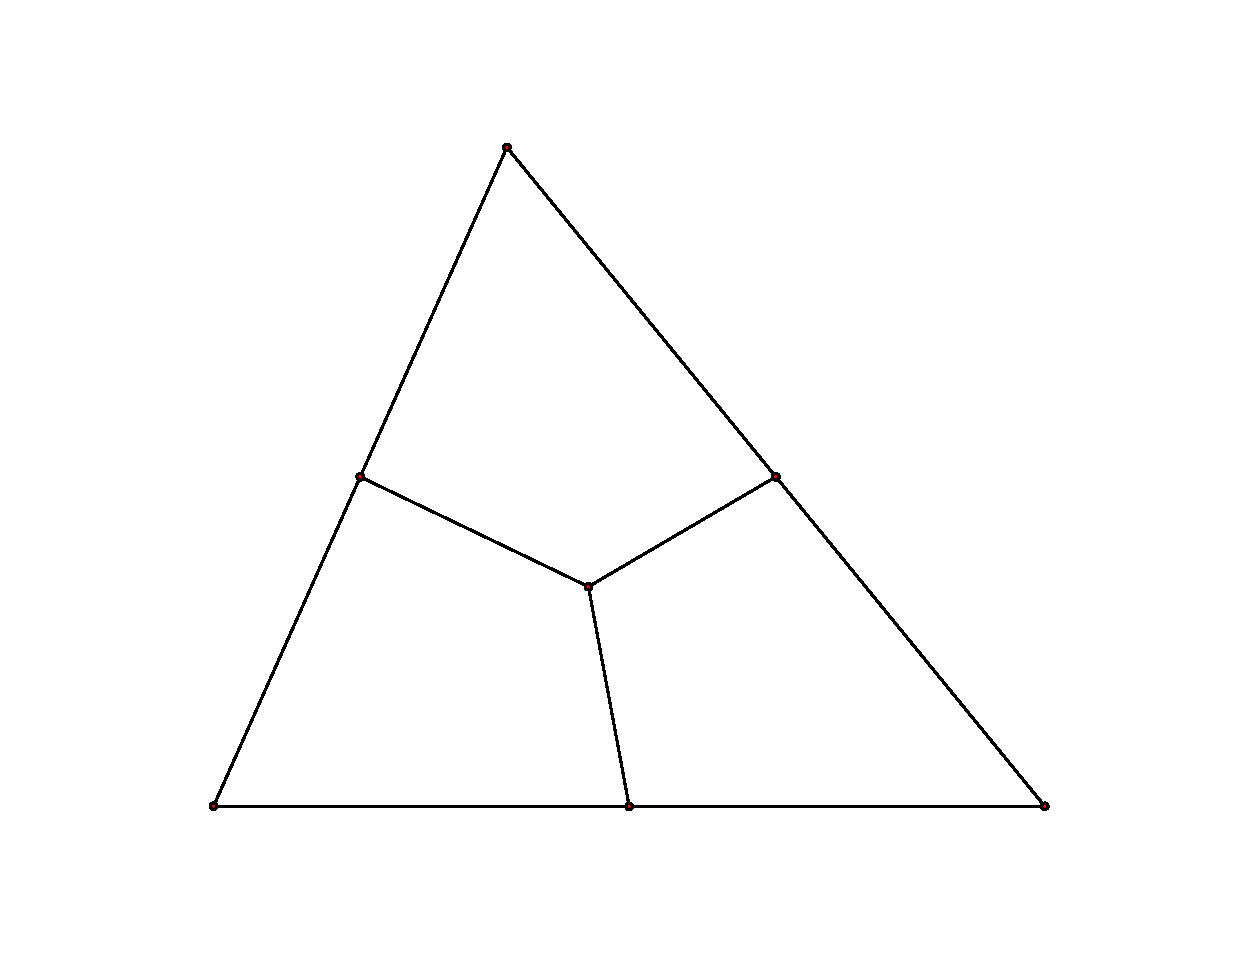
\includegraphics[width=1.2\textwidth]{fig/mesh1.eps}
		\caption{}
		\label{fig:1}
	\end{subfigure}
	\begin{subfigure}[H]{0.49\textwidth}
		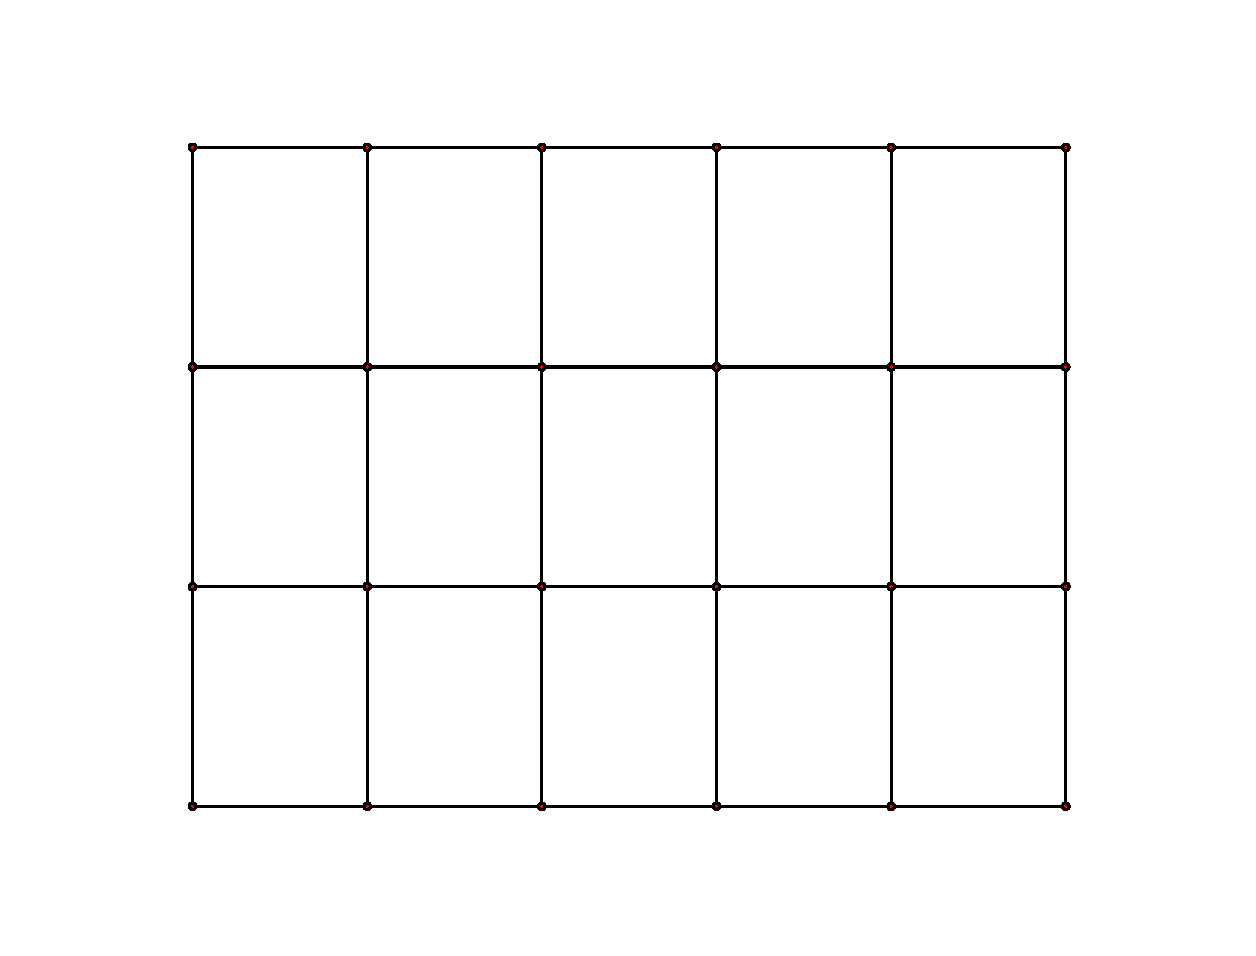
\includegraphics[width=\textwidth]{fig/mesh2.eps}
		\caption{}
		\label{fig:2}
	\end{subfigure}
	\caption{fig(a) is a general shape mesh and fig(b) is a regular rectangular mesh, both with quadrilateral elements.}
	\label{fig:3_1}
\end{figure}

The mesh is created as a module (a different file). The module has its attributes. The main attribute of the module is to instantiate a mesh geometry and its properties, then we can instantiate a regular mesh or a general shape. When a class instantiate something, an object is created. This object, mesh, contains attributes that can be used later.

The general shape mesh is created using Gmsh. Gmsh is copyright \copyright 1997-2014 by C. Geuzaine and J.-F. Remacle. Gmsh is a free to use software and can be distributed under the General Public License (GPL).

\subsubsection{Gmsh}

The first step for generate a mesh is to create the outside nodes. This is done by going to geometry, elementary entities, add, point. Then these points are connected with straight lines. The second step is to define a plane surface. Third is to create physical groups, lines for boundary conditions and surface that will generate a connectivity matrix for the elements. In order to get quad elements is necessary to specify on the mesh options (tools-options-mesh-general) that the subdivision algorithm is "All Quads". Finally the mesh is created by clicking on the 2D. The size of the elements can be adjusted later on the options menu.


\begin{figure}[H]
\centering
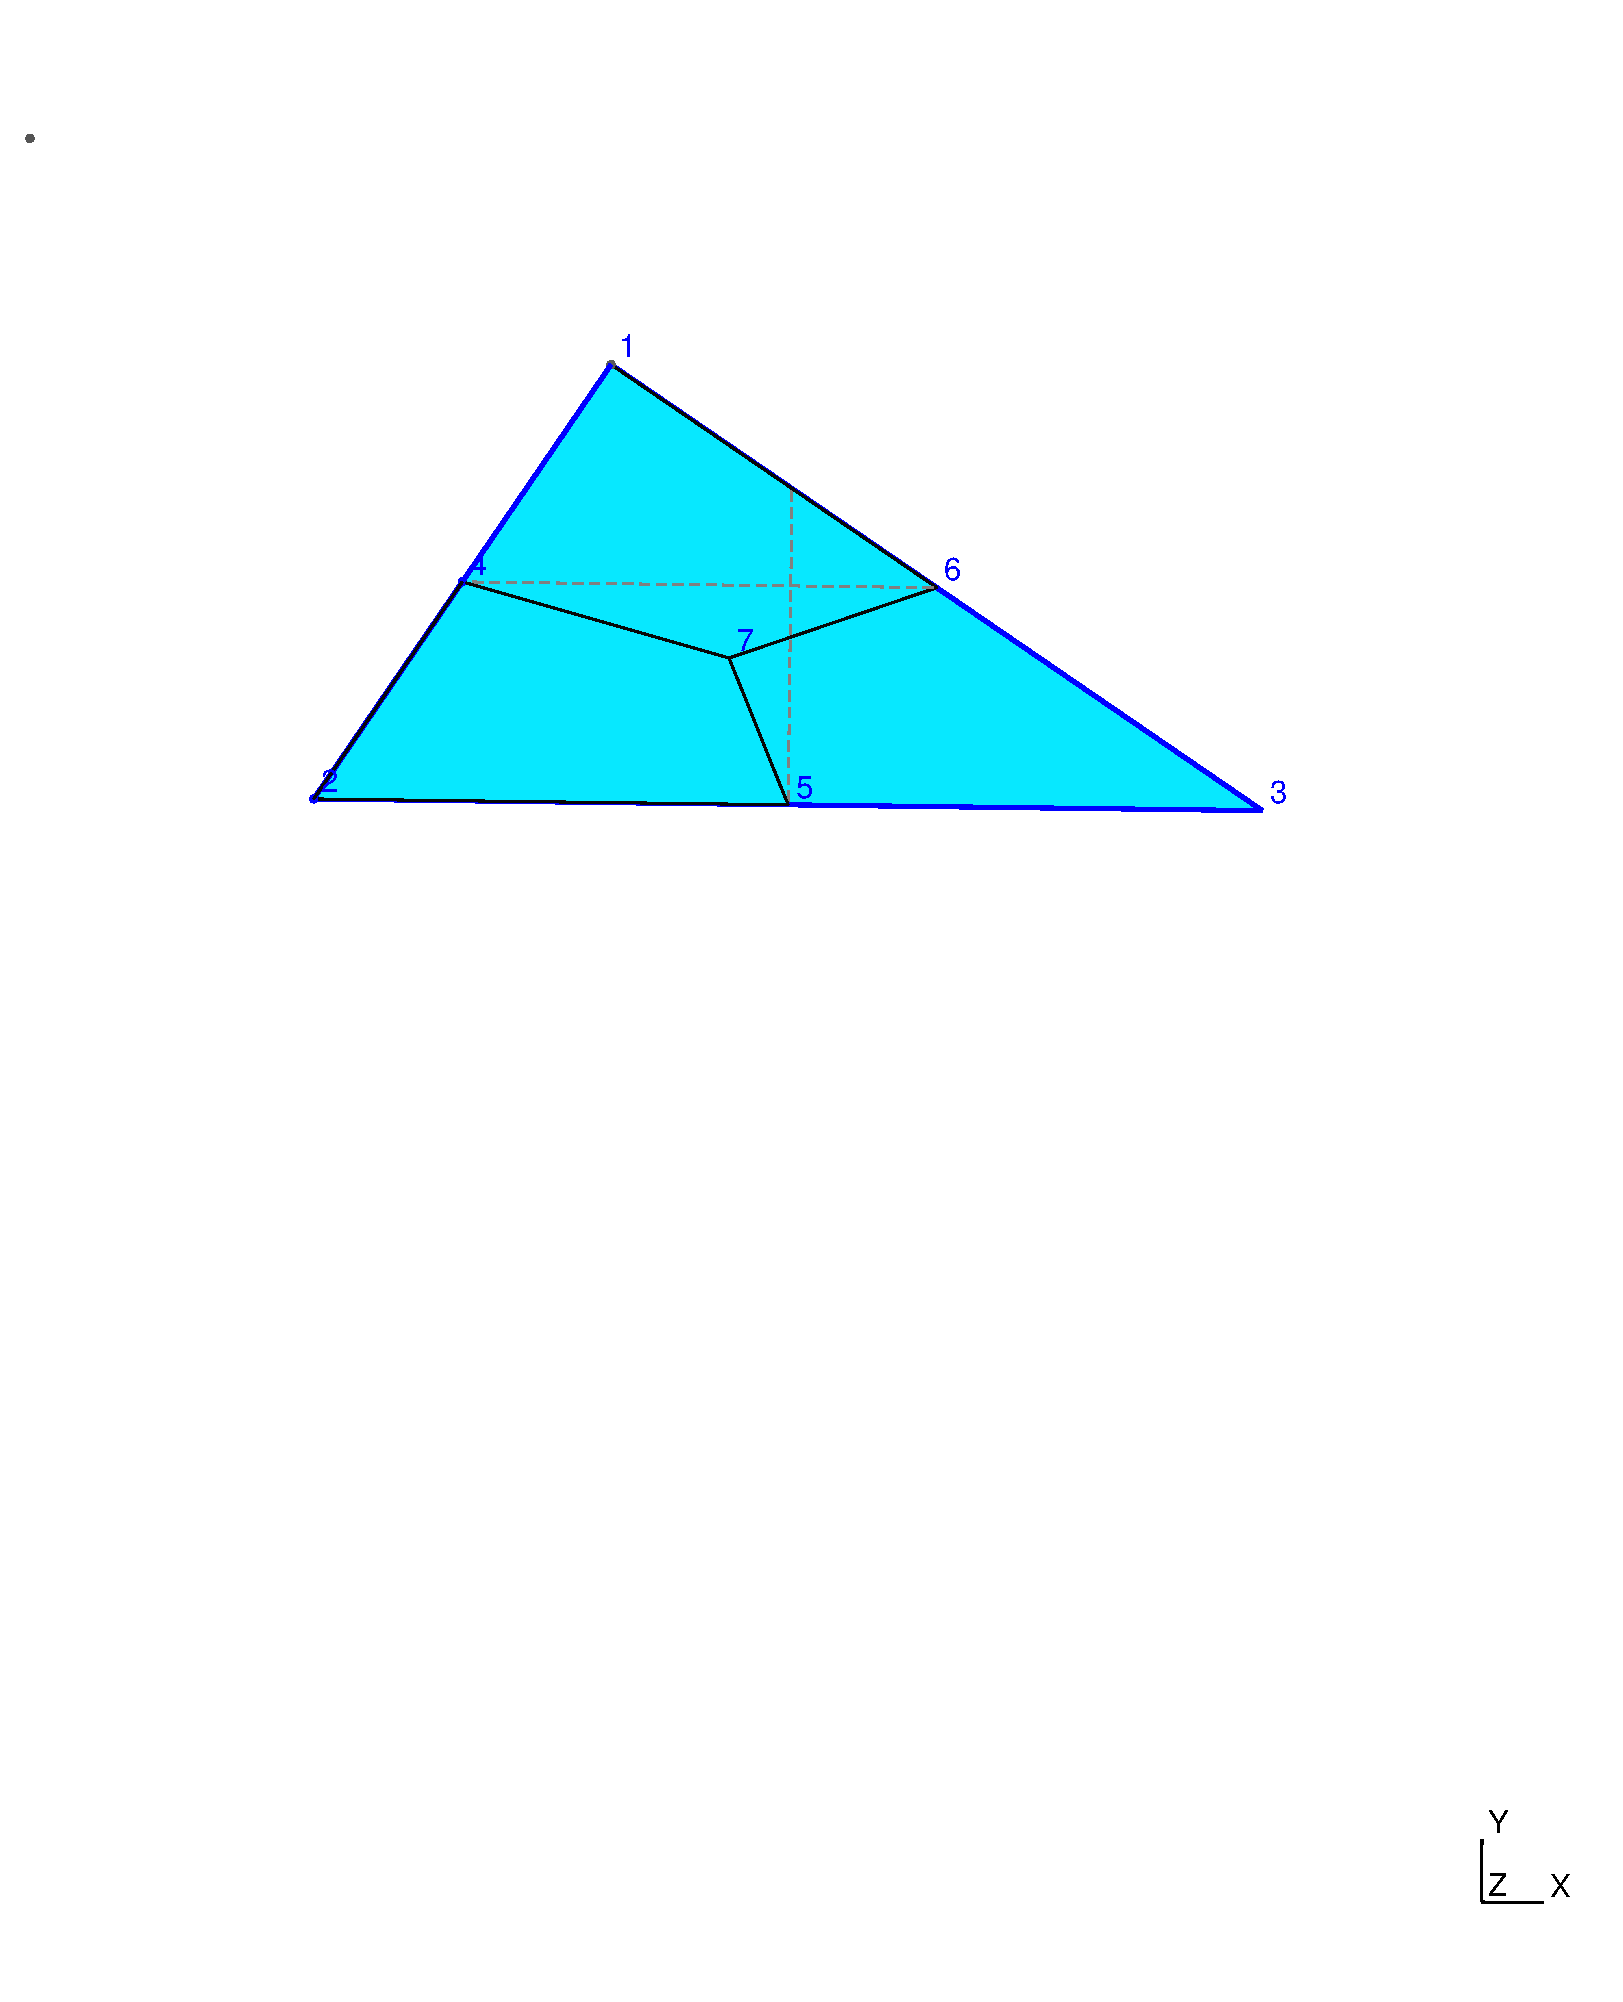
\includegraphics[trim = 0 550 0 100, clip,width=0.8\textwidth]{fig/meshgmsh.eps}
\caption{Mesh generated with gmsh.}
\end{figure}

\subsubsection{Module}

The mesh module contain a class that can be instantiate into a variable object. This mesh object has automatically intrinsic properties (because of the init method). Those properties are: the coordinates of the nodes arranged in a second order array with two columns and as many rows as the number of nodes; the connectivity matrix arranged in a second order array with 4 columns (quad elements) and as many rows as the number of elements. These properties corresponds to data attributes to the instance object mesh.

The mesh object also have method attributes ---\textsf{ Meshname.attribute() }--- which are functions that can be called with the intuitive namespace. For example, when computing each of the components of the matrix we call a method that computes the Jacobian for each element, individually, with the nodes that define the element as argument for each Gauss point.


\subsubsection{Methods}

\paragraph{\textsf{basisFunction2D}} which adds new attributes to the object. Those new attributes are: a first order array with the linear shape functions in 2-dimensions at a specific Gauss point.

\begin{equation*}
\textsf{mesh.phi} = \begin{bmatrix}
\phi^1(g_p, g_w) & \phi^2(g_p, g_w) & \phi^3(g_p, g_w) & \phi^4(g_p, g_w)
\end{bmatrix}^T
\end{equation*}

the second one is a second order array with the derivative of the shape functions with respect to the first and second natural coordinates (in the isoparametric domain).

\begin{equation*}
\textsf{mesh.dphi} = \begin{bmatrix}
\phi^1_{,\xi_1} & \phi^2_{,\xi_1} & \phi^3_{,\xi_1} & \phi^4_{,\xi_1}\\[.2cm]
\phi^1_{,\xi_2} & \phi^2_{,\xi_2} & \phi^3_{,\xi_2} & \phi^4_{,\xi_2}
\end{bmatrix}
\end{equation*}

\paragraph{\textsf{mapping}} changes the variable from the Cartesian coordinates into the natural domain, this is done by using

\begin{equation*}
x_i = \sum_k^4 \chi^k_i \phi^k,
\end{equation*}

or,

\begin{equation*}
\begin{bmatrix}
x_1 \\[.2cm]
x_2
\end{bmatrix} = \begin{bmatrix}
\chi^1_1 \\[.2cm]
\chi^1_2
\end{bmatrix} \phi^1 +
\begin{bmatrix}
\chi^2_1 \\[.2cm]
\chi^2_2
\end{bmatrix} \phi^2
\begin{bmatrix}
\chi^3_1 \\[.2cm]
\chi^3_2
\end{bmatrix} \phi^3
\begin{bmatrix}
\chi^4_1 \\[.2cm]
\chi^4_2
\end{bmatrix} \phi^4,
\end{equation*}

where, $\chi^k_i$ represent the $k$ node coordinate $i$ of an individual element (with 4 nodes). The Cartesian coordinates will be a function of the natural coordinates, $x_i(\xi_j)$. The mapping is done so we can compute the integrals on the isoparametric domain using Gaussian Quadrature. This method is called when a integral is computed, inside a \textsf{for} loop.

\paragraph{eleJacobian}

This method creates a series of attributes related with the Jacobian matrix generated on the process of changing variables. It is called when a integral is calculated. The first attribute is the Jacobian matrix, expressed earlier. This matrix is obtained by the following multiplication

\begin{equation*}
\mathsf{mesh.Jac} = \begin{bmatrix}
\phi^1_{,\xi_1} & \phi^2_{,\xi_1} & \phi^3_{,\xi_1} & \phi^4_{,\xi_1} \\[.2cm]
\phi^1_{,\xi_2} & \phi^2_{,\xi_2} & \phi^3_{,\xi_2} & \phi^4_{,\xi_2}
\end{bmatrix}
\begin{bmatrix}
\chi^1_1 & \chi^1_2 \\[.2cm]
\chi^2_1 & \chi^2_2 \\[.2cm]
\chi^3_1 & \chi^3_2 \\[.2cm]
\chi^4_1 & \chi^4_2 
\end{bmatrix},
\end{equation*} 

note that the Jacobian matrix is already in the natural coordinates. The next attribute is the determinant of this matrix, $\textsf{mesh.detJac}$. 

In order to use the chain rule we need the inverse of the Jacobian matrix, this is done by using a method from \textsf{NumPy} library.

The calculation of the entries of the stiffness matrix require the derivative of the shape functions with respect to the Cartesian coordinates. Because the coordinte system has changed, the derivative must be calculated with the chain rule. The attribute builds an 2x4 array with the gradient of each shape function, this is done by multiplying

\begin{equation*}
\textsf{mesh.dphi}\_\textsf{xi} = \begin{bmatrix}
\xi_{1,x_1} & \xi_{2,x_1} \\[.2cm]
\xi_{1,x_2} & \xi_{2,x_2}
\end{bmatrix}
 \begin{bmatrix}
\phi^1_{,\xi_1} & \phi^2_{,\xi_1} & \phi^3_{,\xi_1} & \phi^4_{,\xi_1} \\[.2cm]
\phi^1_{,\xi_2} & \phi^2_{,\xi_2} & \phi^3_{,\xi_2} & \phi^4_{,\xi_2}
\end{bmatrix}
\end{equation*}

\paragraph{\textsf{ArchLength}}

This attributes to the object a vector with the 4 arch length for the change in coordinates on the line integral. From the Jacobian matrix,

\begin{equation*}
\textsf{mesh.Jac} = \begin{bmatrix}
x_{1,\xi_1} & x_{2,\xi_1} \\
x_{1,\xi_2} & x_{2,\xi_2} 
\end{bmatrix},
\end{equation*}

the arch length ratios are,

\begin{equation*}
\textsf{mesh.ArchLength} = \begin{bmatrix}
\sqrt{\textsf{mesh.Jac}[1,0]^2 + \textsf{mesh.Jac}[1,1]^2} \\[.2cm]
\sqrt{\textsf{mesh.Jac}[0,0]^2 + \textsf{mesh.Jac}[0,1]^2} \\[.2cm]
\sqrt{\textsf{mesh.Jac}[1,0]^2 + \textsf{mesh.Jac}[1,1]^2} \\[.2cm]
\sqrt{\textsf{mesh.Jac}[0,0]^2 + \textsf{mesh.Jac}[0,1]^2}
\end{bmatrix} = \begin{bmatrix}
\sqrt{x_{1,\xi_2}^2 + x_{2,\xi_2}^2} \\[.2cm]
\sqrt{x_{1,\xi_1}^2 + x_{2,\xi_1}^2} \\[.2cm]
\sqrt{x_{1,\xi_2}^2 + x_{2,\xi_2}^2} \\[.2cm]
\sqrt{x_{1,\xi_1}^2 + x_{2,\xi_1}^2} 
\end{bmatrix}
\end{equation*}

The first entry is refereed to right side of the element with $\xi_1=1$, the second: top side with $\xi_2=1$, the third: left side with $\xi_1=-1$ and lastly the fourth: bottom side with $\xi_2=-1$.

\subsection{Stiffness Matrix}



Using Gaussian Quadrature (GQ) with two points on each direction, the integral becomes
\begin{align*}
K_{mn} &=  \int_{\Omega} \phi_{m,i} k \phi_{n,i}  \, \mathrm{d}\Omega  \\
		&= k \int_{-1}^1 \int_{-1}^1 \phi(\xi_j)_{m,u} \; \xi_{u,i} \; \phi(\xi_j)_{n,v} \; \xi_{v,i} \; \det[x_{r,t}]  \, \mathrm{d}\xi_1 \mathrm{d}\xi_2 \\
		&= k \int_{-1}^1 \int_{-1}^1 \phi(\xi_j)_{m,u} \; \xi_{u,i} \; \phi(\xi_j)_{n,v} \; \xi_{v,i} \; \det[x_{r,t}]\, \mathrm{d}\xi_1 \mathrm{d}\xi_2 \\
		&= k \sum_{p=1}^2 \sum_{w=1}^2 \phi(g_p, g_w)_{m,u} \; \xi(g_p, g_w)_{u,i}  \; \phi(g_p, g_w)_{n,v} \; \xi(g_p, g_w)_{v,i} \; \det[x_{r,t}](g_p, g_w),
\end{align*}
where, $i,j,u,v,r,t=1,2$, i.e., all those indexes go from 1 to 2. All terms are functions of variables in the natural coordinate system and they are going to be evaluated at the 4 combination of GQ points, $(g_p, g_w)$. The stiffness matrix will be a size $4x4$, combination of $m,n =1,2,3,4$. The implementation is made through a matrix multiplication
\begin{equation*}
\mathbf{K} = \sum_{p=1}^2 \sum_{w=1}^2 k\mathbf{B^T} \mathbf{B} \det[x_{r,t}](g_p, g_w),
\end{equation*}
where,
\begin{equation*}
\mathbf{B} =  \begin{bmatrix}
\dfrac{\urpartial \phi_1}{\urpartial x_1} & \dfrac{\urpartial \phi_2}{\urpartial x_1} & \dfrac{\urpartial \phi_3}{\urpartial x_1} & \dfrac{\urpartial \phi_4}{\urpartial x_1} \\[.4cm]
\dfrac{\urpartial \phi_1}{\urpartial x_2} & \dfrac{\urpartial \phi_2}{\urpartial x_2} & \dfrac{\urpartial \phi_3}{\urpartial x_2} & \dfrac{\urpartial \phi_4}{\urpartial x_2} 
\end{bmatrix}
\end{equation*}

\subsection{Load Vector}


The next integral can be divided in two parts: $R_m = R_m + T_m$. The first refer to the internal heat source and the second to the boundary flux condition. Then
\begin{align*}
R_m &= \int_\Omega  \phi(x_i)_m q(x_i)   \, \mathrm{d}\Omega \\
	&= \int_{-1}^1 \int_{-1}^1 \phi(x_i(\xi_j))_m \; q(x_i(\xi_j)) \; \det[x_{r,t}]\, \mathrm{d}\xi_1 \mathrm{d}\xi_2 \\
	&= \int_{-1}^1 \int_{-1}^1 \phi(\xi_j)_m \; q(\xi_j) \; \det[x_{r,t}]\, \mathrm{d}\xi_1 \mathrm{d}\xi_2 \\ 
	&= \sum_{p=1}^2 \sum_{w=1}^2 \phi(g_p, g_w)_m \; q(g_p, g_w) \; \det[x_{r,t}](g_p, g_w).
\end{align*}
The vector $R_m$ has dimension $m$. 

\subsection{Traction Vector}


For the second part the term $k \theta_{,x_i} = t$ represents the flux value for the boundary points,  $x_i \in \urpartial \Omega$.
\begin{align*}
T_m &= \int_{\urpartial \Omega} \phi(x_i)_m \; t(x_i) \, \mathrm{d}\Gamma\\
	&= \sum_{k=1}^4 \int_{\urpartial \Omega^k} \phi(x_i)_m \; t(x_i) \, \mathrm{d}\Gamma^k.
\end{align*}
For each element side, we can map the Cartesian coordinates into the natural domain. The Jacobian will be the ration between arc lengths.
\begin{align*}
j=1 \qquad \mathrm{d} \Gamma^1 = \sqrt{x_{1,\xi_2}^2 + x_{2,\xi_2}^2} \mathrm{d}\xi_2 ;\\
j=2 \qquad \mathrm{d} \Gamma^2 = \sqrt{x_{1,\xi_1}^2 + x_{2,\xi_1}^2} \mathrm{d}\xi_1; \\
j=3 \qquad \mathrm{d} \Gamma^3 = \sqrt{x_{1,\xi_2}^2 + x_{2,\xi_2}^2} \mathrm{d}\xi_2 ;\\
j=4 \qquad \mathrm{d} \Gamma^4 = \sqrt{x_{1,\xi_1}^2 + x_{2,\xi_1}^2} \mathrm{d}\xi_1.
\end{align*}

The integral for the first side is
\begin{align*}
\int_{\urpartial \Omega^1} \phi(x_i(\xi_j))_m \; t(x_i(\xi_j)) \mathrm{d} \Gamma^1 &= \int_{-1}^1 \phi(\xi_j)_m \; t(\xi_j) \sqrt{x_{1,\xi_2}^2 + x_{2,\xi_2}^2} \mathrm{d}\xi_2 \\
&=  \int_{-1}^1 \phi(1, \xi_2)_m\; t(1, \xi_2)   \sqrt{x_{1,\xi_2}^2 + x_{2,\xi_2}^2} \mathrm{d}\xi_2 \\
&=  \sum_{w=1}^2 \phi(1, g_w)_m \; t(1, g_w) \sqrt{x(1, g_w)_{1,\xi_2}^2 + x(1, g_w)_{2,\xi_2}^2}.
\end{align*}

If an element has only one side at the boundary, for instance the element with connectivity $[1, \;5, \; 13, \; 14, \;]$ has a side $[1, \; 5]$ at the boundary. On the mesh module the attribute \textsf{boundary\_ elements} will say that this is the first element, and its first side is on the boundary, $[0, \;0]$.  Then, if we loop over an the elements on the boundary with the information of which side is relevant to the traction vector.


\subsection{Mass Matrix}

The implementation process consists in first change the variables from Cartesian to the isoparametric domain. The shape functions should be evaluated as a function of the isoparametric coordinates at each Gauss point.

\subsection{Boundary Conditions}

The following architecture will be used as a preliminary way of implementing the gmsh file on the already built code. A new module \textsf{Boundaryconditions} is going to be created to not interfere with the already built one.

\begin{enumerate}
\item[1] The gmsh export a \textsf{.geo} text file which contains the straight lines index. (ex: Line(1) = {1, 2}, the line with index (6) is defined between node(1) and Node(2).)
\item[2] The \textsf{.msh} file contain Physical groups assign during the mesh construction. Physical groups are points, lines and planes. Adding lines will produce a set of 7 numbers. (Ex: 1 1 2 6 1 1 4; 1: first element; 1: element type for a line; 2: indicates that there are two tags; 6: first tag that indicates which physical line the element is, this case the element in at Physical Line(6); 1: second tag indicates which line the element is, Line(1); the last two numbers are the nodes of the mesh in the physical line.
\item[3] The difference between Line and Physical Line is: a Line is defined when creating the boundary of the domain whereas a Physical Line is defined when we want to know the nodes of the mesh contained on that specific line for apply boundary conditions.
\item[4] The program will print all the lines presented in the geometry boundary and its indexes ([1 , 2, 3]: lines 1, 2 and 3 are part of the boundary).
\item[5] Then, the user will define for each line a type of boundary, Dirichlet or Neumann (1 - D: line 1 will have Dirichlet BC). Line(1) on the \textsf{.msh} will have a tag right before the nodes indexed (Ex: 1 1 2 6 \underline{1} 1 4, so Dirichlet boundary conditions must be applied on degrees of freedom of Node(1) and Node(4)).
\item[6] Then the value of the BC is defined.
\end{enumerate}

An array with the boundary lines and nodes is extracted from the \textsf{.msh} file with the following format,

\begin{equation*}
\textsf{boundary}\_\textsf{nodes} = \begin{bmatrix}
1 & 1 & 4
\end{bmatrix},
\end{equation*}

the first column indicates that the element nodes are at Line(1), the other two number indicates that Node(1) and Node(4) are on this boundary.

idea: The dirichlet BC can be applied directly on the boundary nodes. 

Note that the Neumann boundary condition can't overlap with Dirichlet ones.

\section{Results}

\subsection{Dirichlet Conditions}

\begin{figure}[H]
\centering
	\begin{subfigure}[H]{0.5\textwidth}
		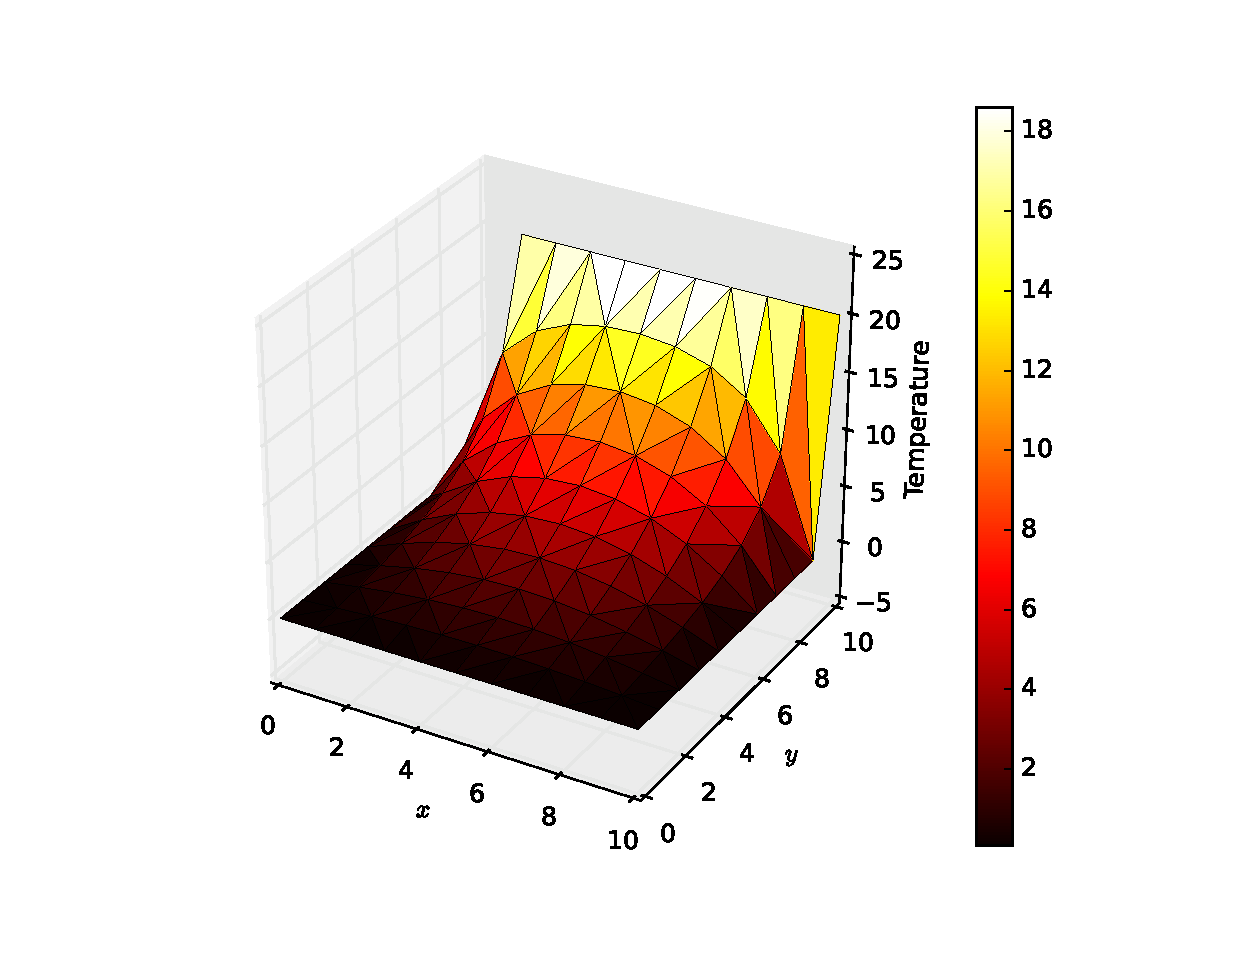
\includegraphics[width=1.2\textwidth]{fig/figure_1.eps}
		\caption{}
		\label{fig:1}
	\end{subfigure}
	\begin{subfigure}[H]{0.3\textwidth}
		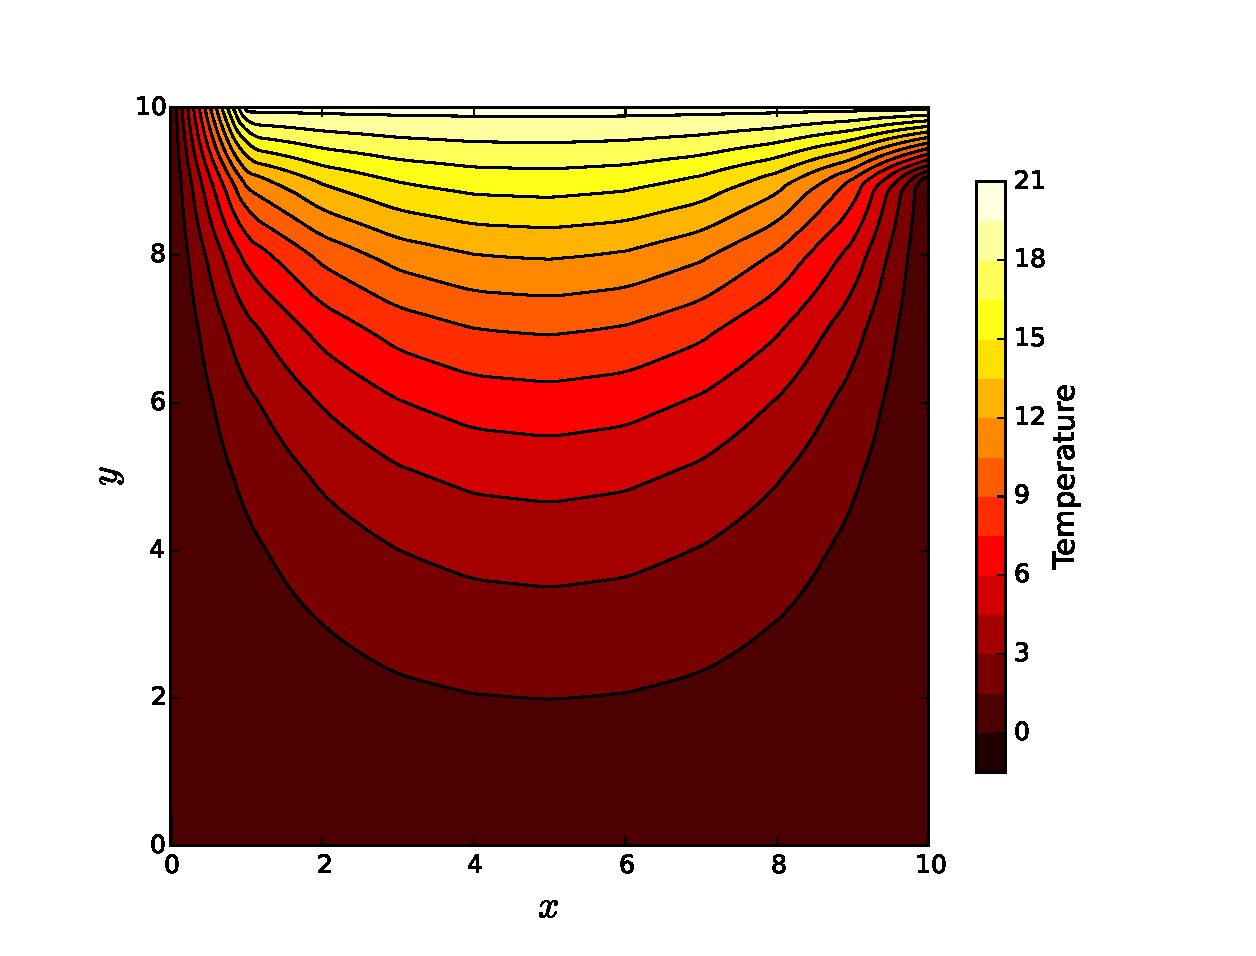
\includegraphics[width=\textwidth]{fig/figure_1.1.eps}
		\caption{}
		\label{fig:2}
	\end{subfigure}
	\caption{10 elements each direction}
	\label{fig:3_1}
\end{figure}

\begin{figure}[H]
\centering
	\begin{subfigure}[H]{0.5\textwidth}
		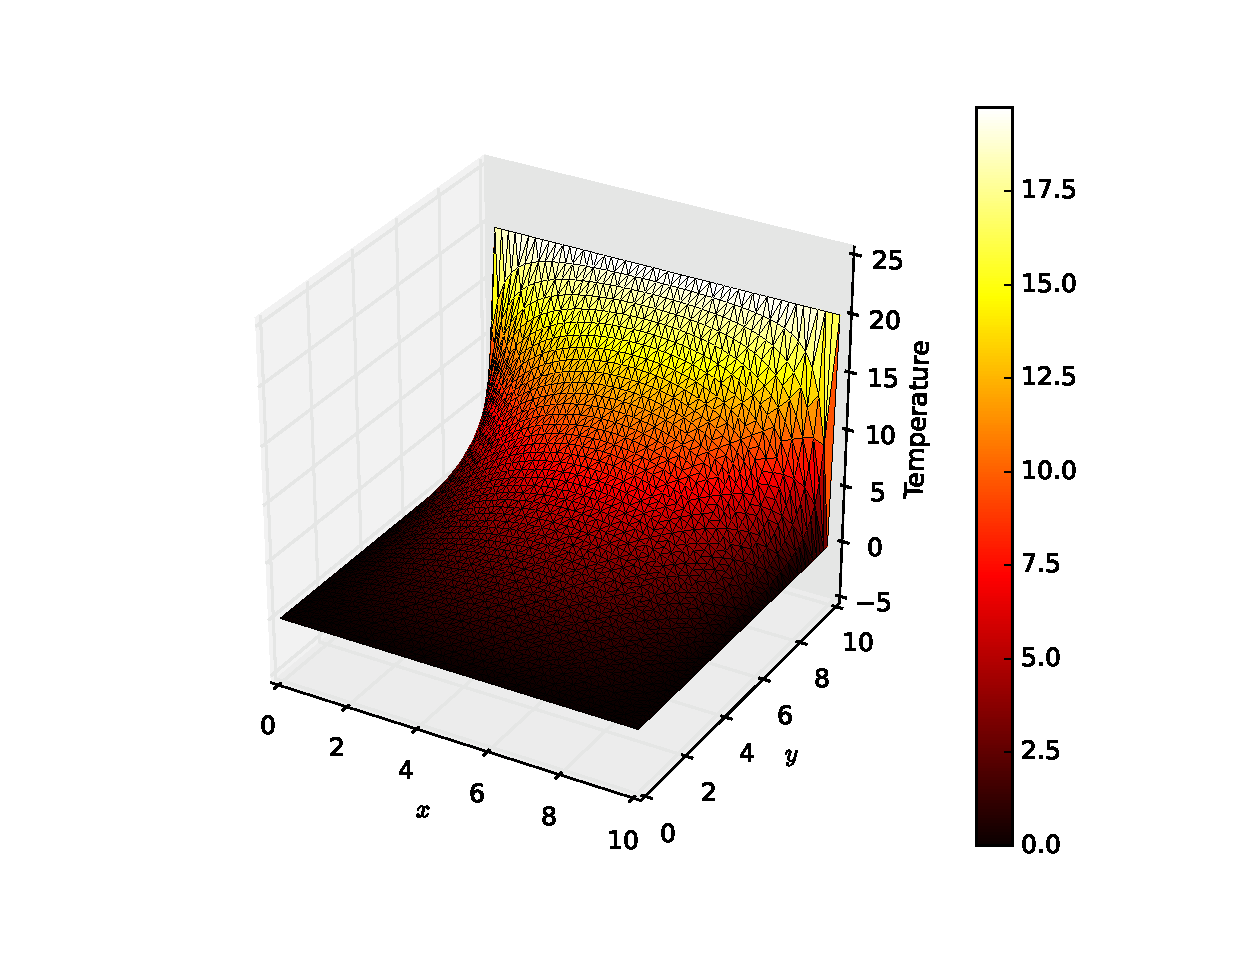
\includegraphics[width=1.2\textwidth]{fig/figure_2.eps}
		\caption{}
		\label{fig:1}
	\end{subfigure}
	\begin{subfigure}[H]{0.3\textwidth}
		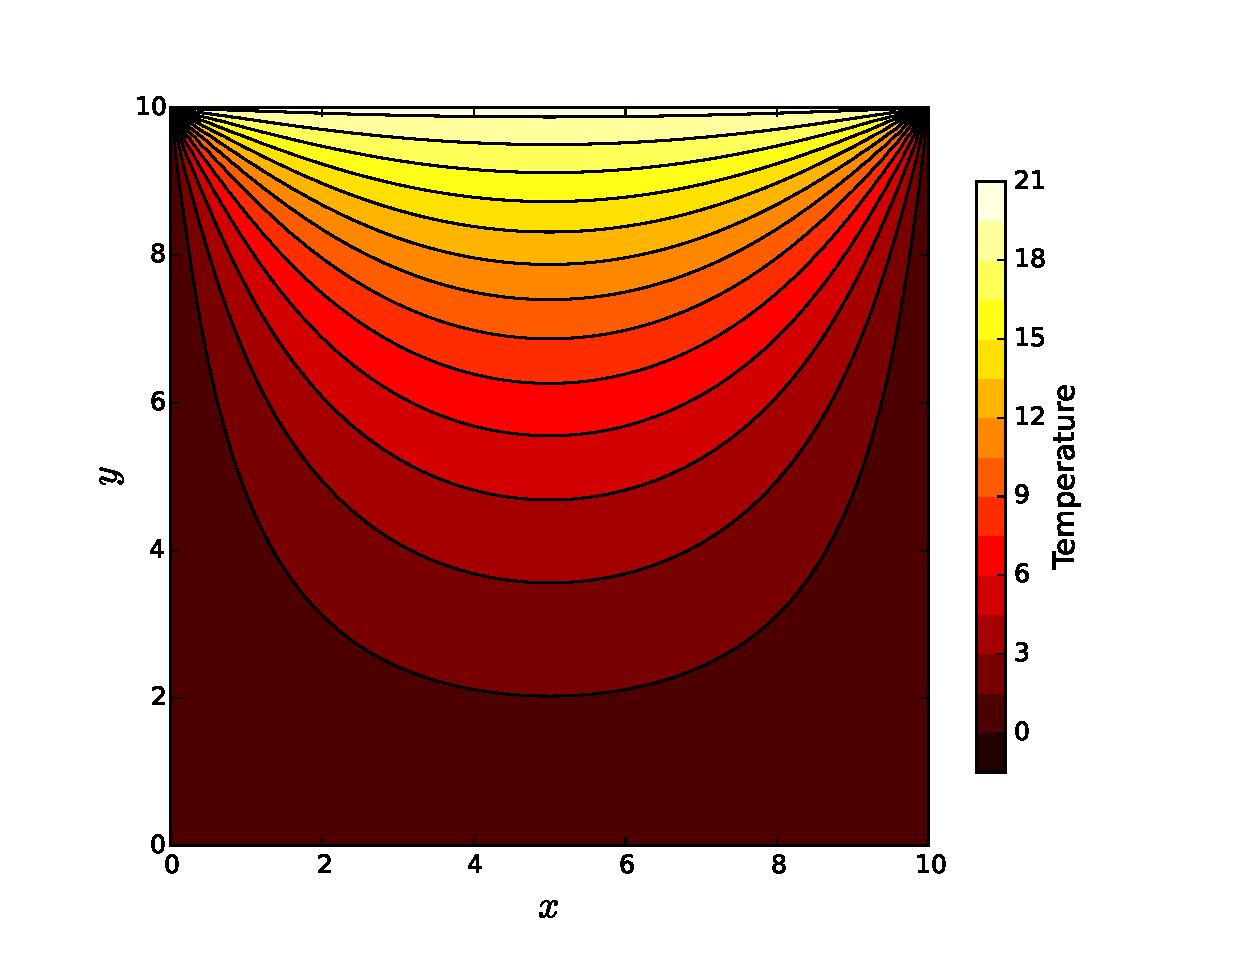
\includegraphics[width=\textwidth]{fig/figure_2.1.eps}
		\caption{}
		\label{fig:2}
	\end{subfigure}
	\caption{50 elements each direction}
	\label{fig:3_1}
\end{figure}




\subsection{Internal Load}

Uniform distributed load equal $q=10$.

\begin{figure}[H]
\centering
	\begin{subfigure}[H]{0.5\textwidth}
		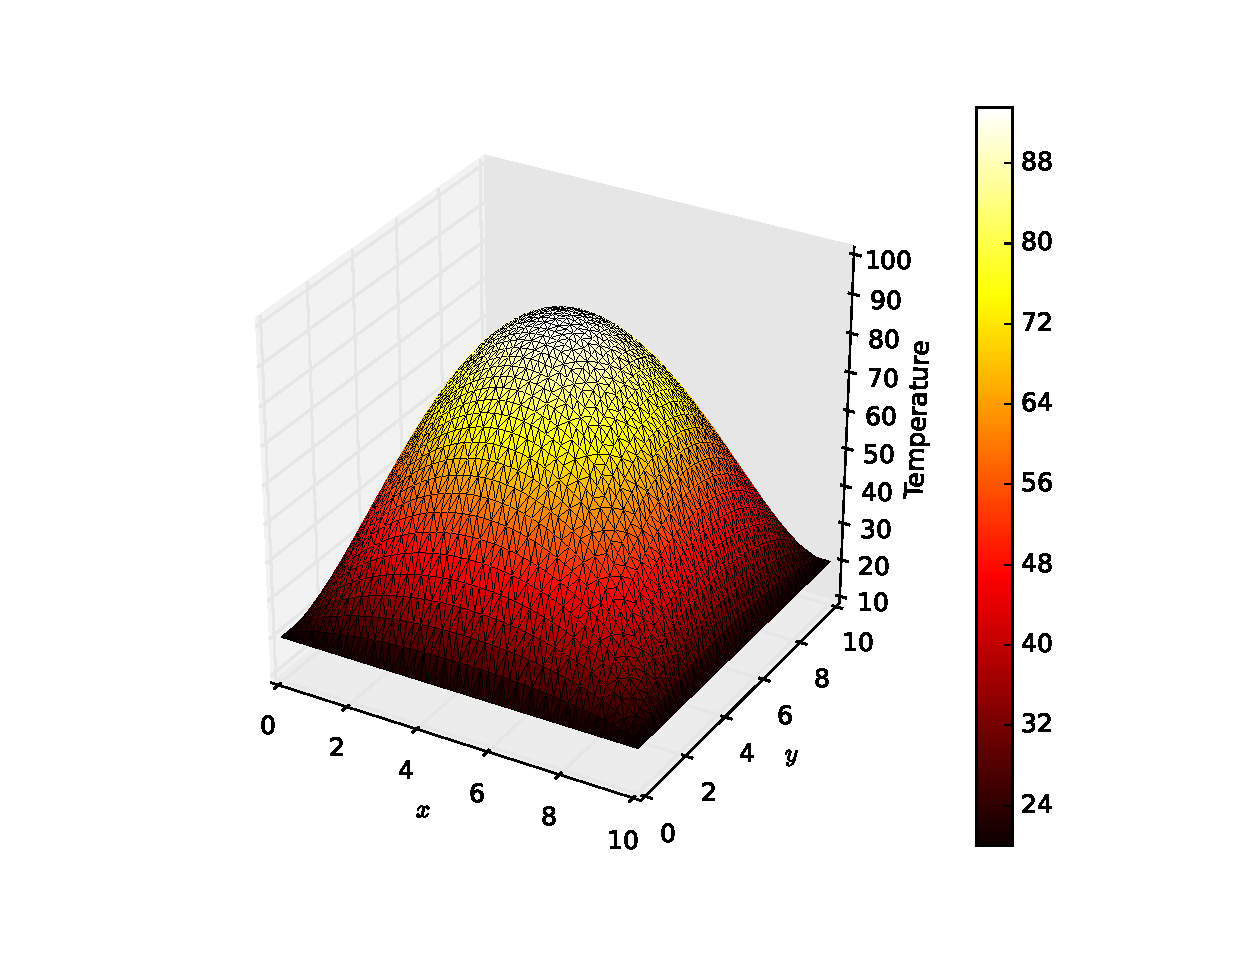
\includegraphics[width=1.2\textwidth]{fig/figure_3.eps}
		\caption{}
		\label{fig:1}
	\end{subfigure}
	\begin{subfigure}[H]{0.3\textwidth}
		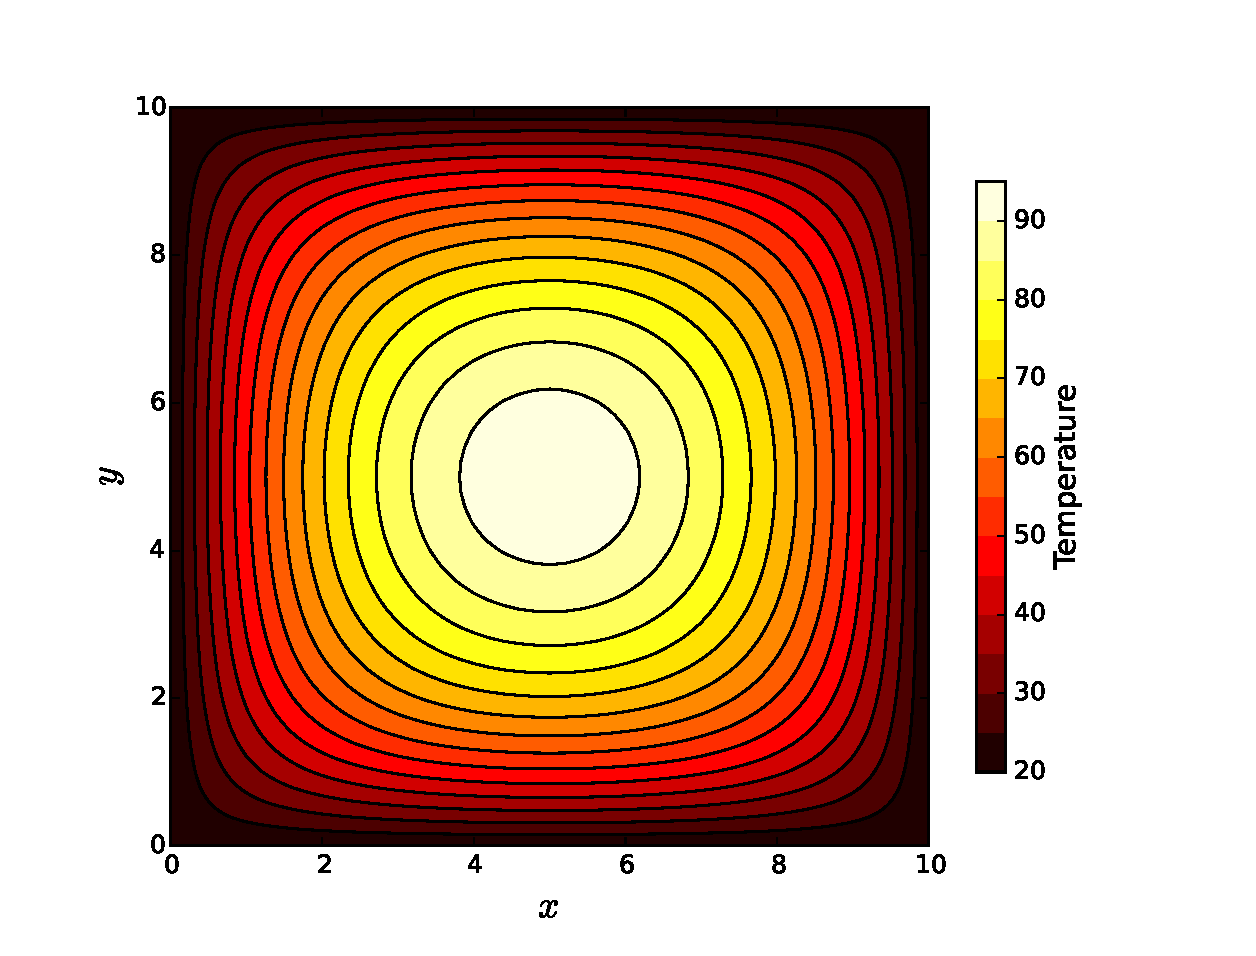
\includegraphics[width=\textwidth]{fig/figure_3.1.eps}
		\caption{}
		\label{fig:2}
	\end{subfigure}
	\caption{50 elements each direction}
	\label{fig:3_1}
\end{figure}

load $q=\sin x \sin y$

\begin{figure}[H]
\centering
	\begin{subfigure}[H]{0.5\textwidth}
		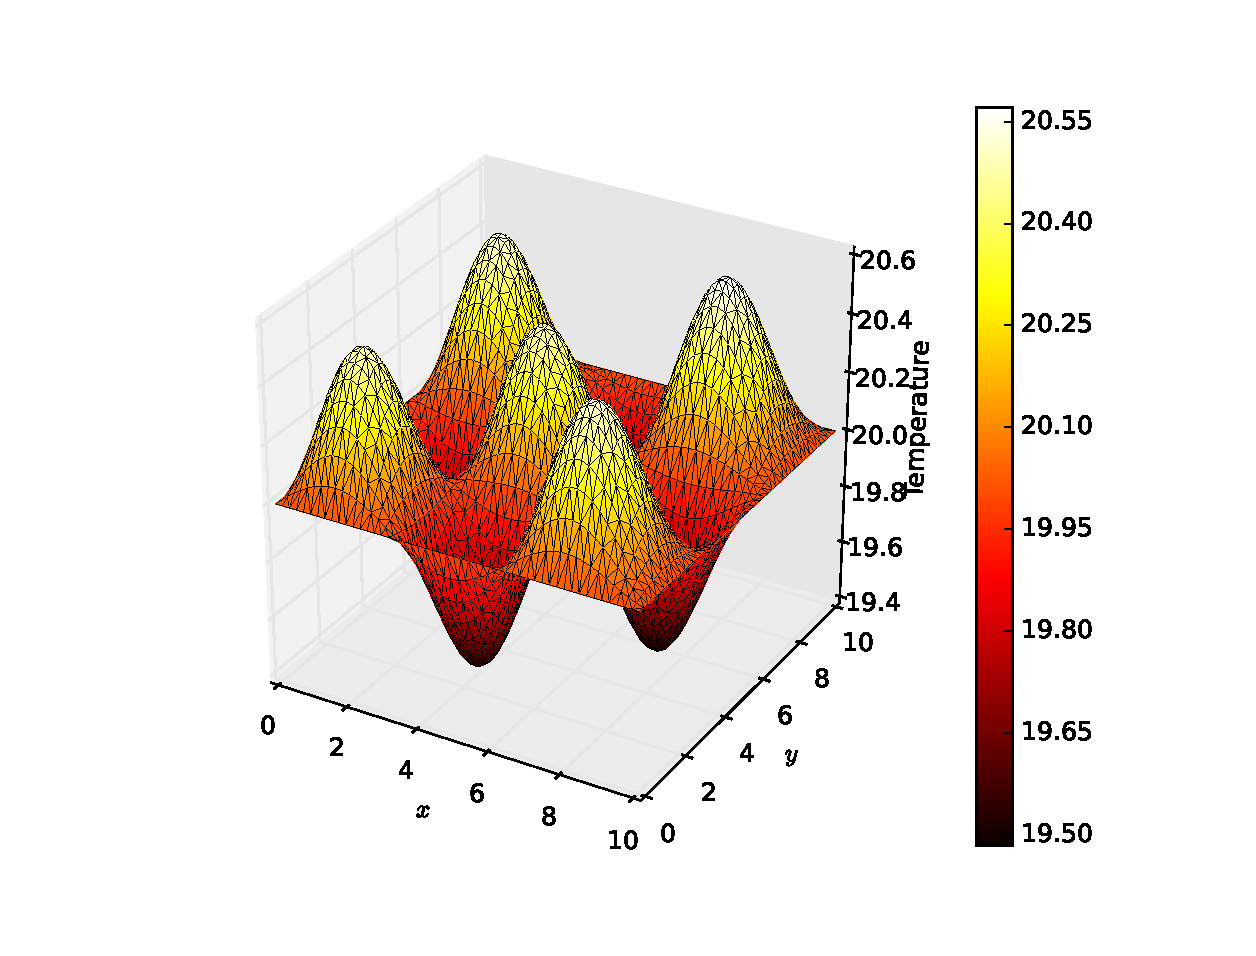
\includegraphics[width=1.2\textwidth]{fig/figure_4.eps}
		\caption{}
		\label{fig:1}
	\end{subfigure}
	\begin{subfigure}[H]{0.3\textwidth}
		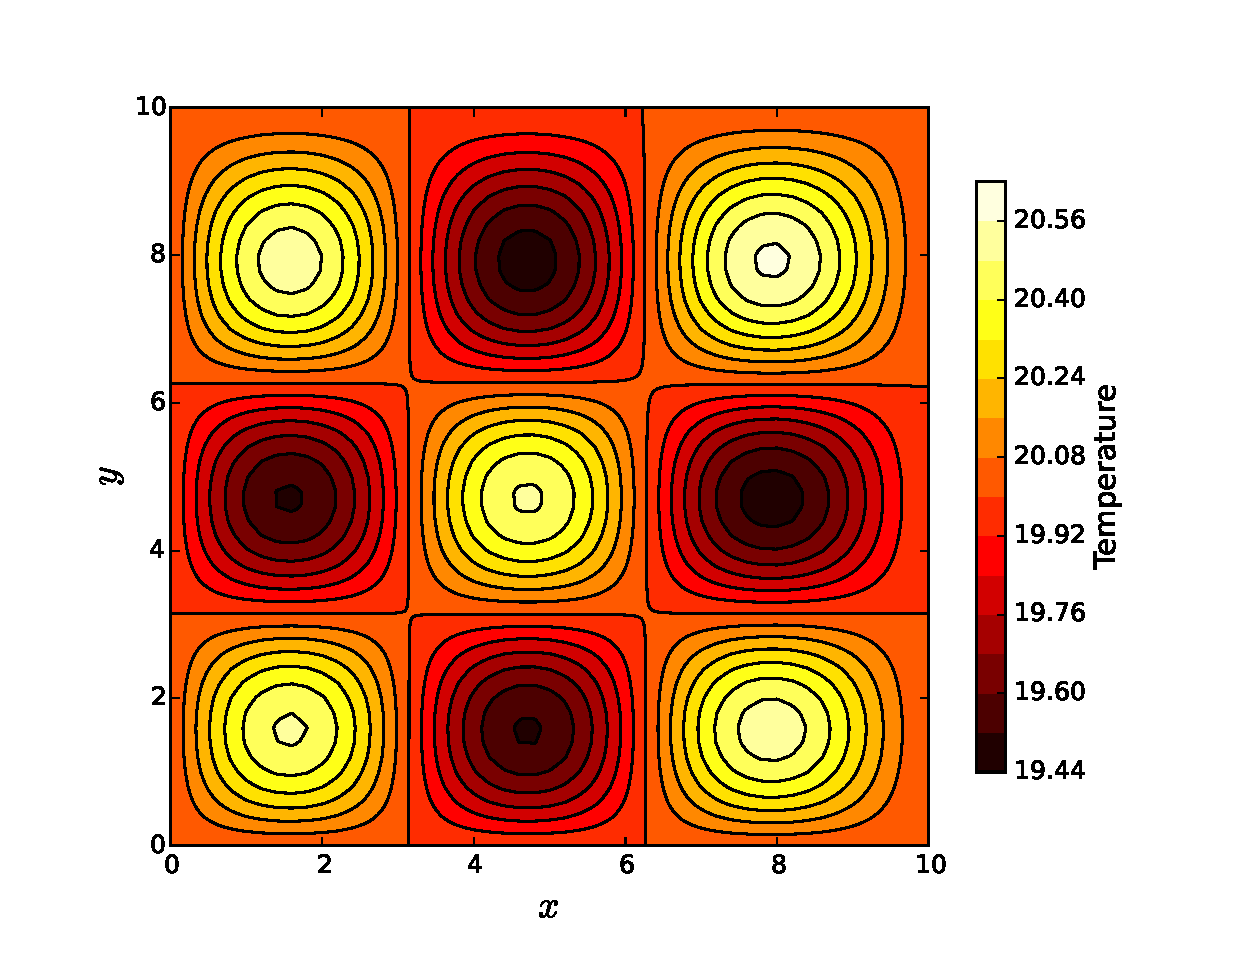
\includegraphics[width=\textwidth]{fig/figure_4.1.eps}
		\caption{}
		\label{fig:2}
	\end{subfigure}
	\caption{50 elements each direction}
	\label{fig:3_1}
\end{figure}

\subsection{Neumann Boundary Condition}

$T = x^2$ on one side and $T=-y^2$ on the other.

\begin{figure}[H]
\centering
	\begin{subfigure}[H]{0.5\textwidth}
		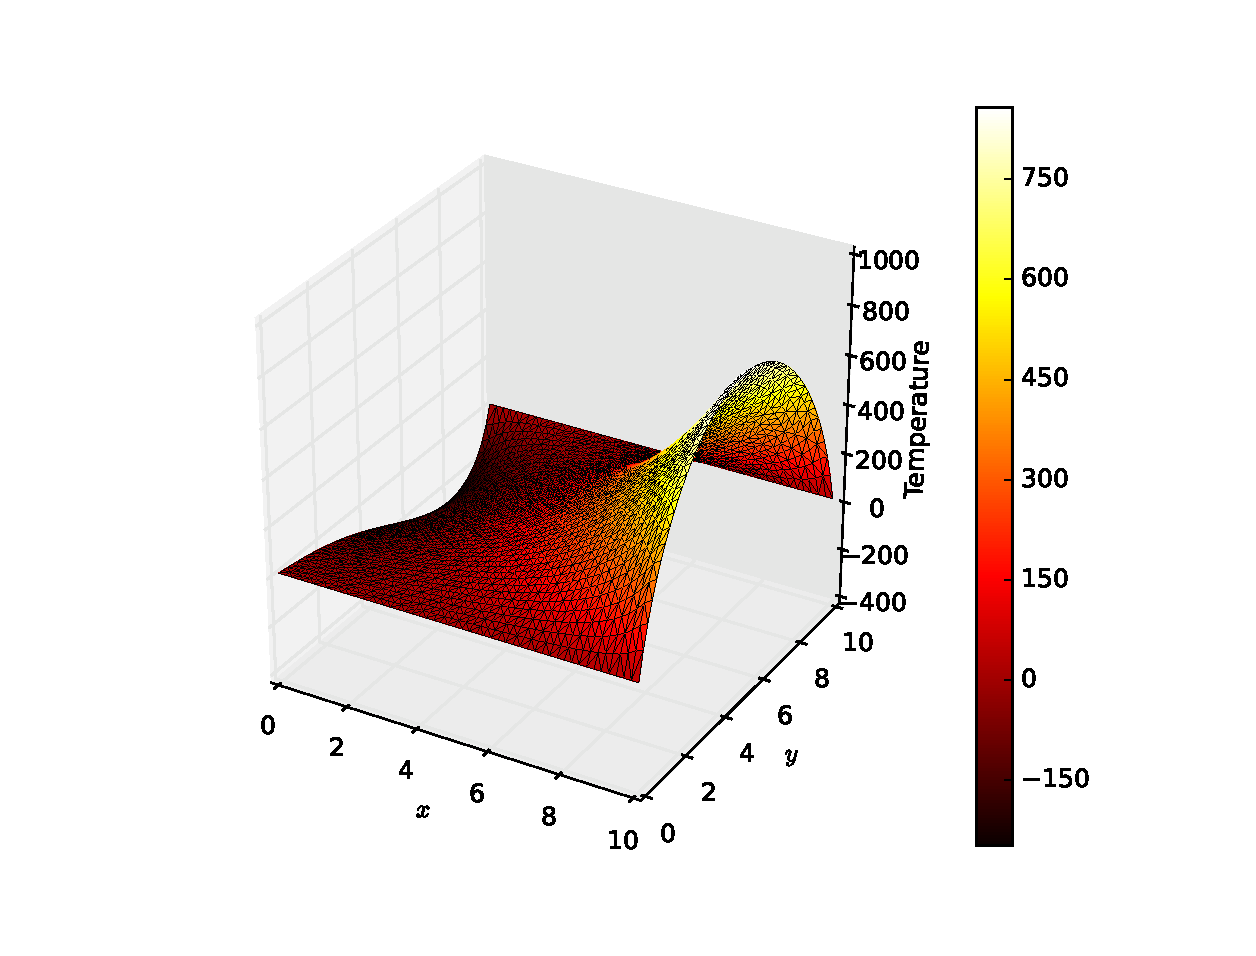
\includegraphics[width=1.2\textwidth]{fig/figure_5.eps}
		\caption{}
		\label{fig:1}
	\end{subfigure}
	\begin{subfigure}[H]{0.3\textwidth}
		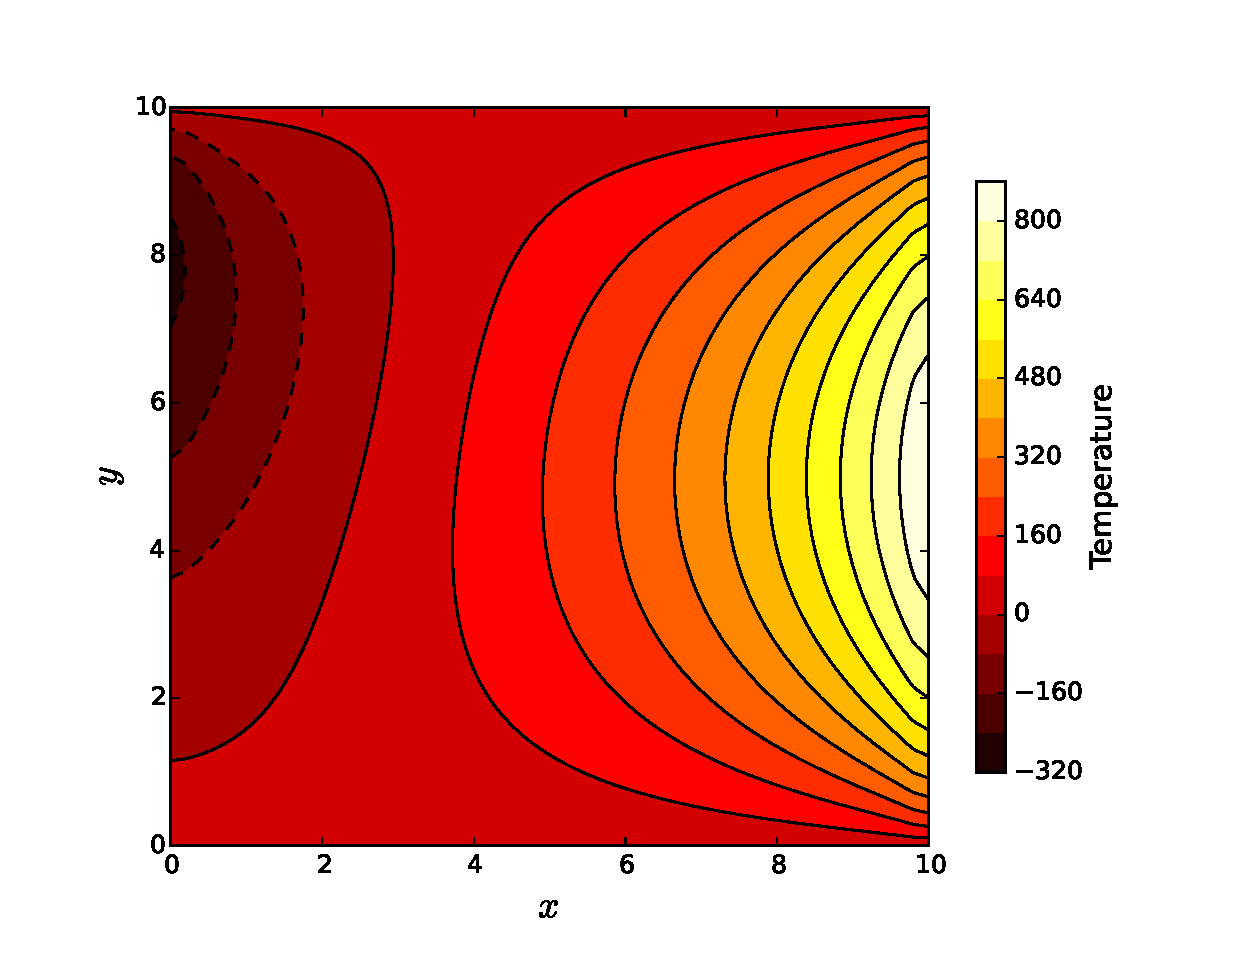
\includegraphics[width=\textwidth]{fig/figure_5.1.eps}
		\caption{}
		\label{fig:2}
	\end{subfigure}
	\caption{50 elements each direction}
	\label{fig:3_1}
\end{figure}

\subsection{General materials}

\begin{figure}[H]
\centering
	\begin{subfigure}[H]{0.5\textwidth}
		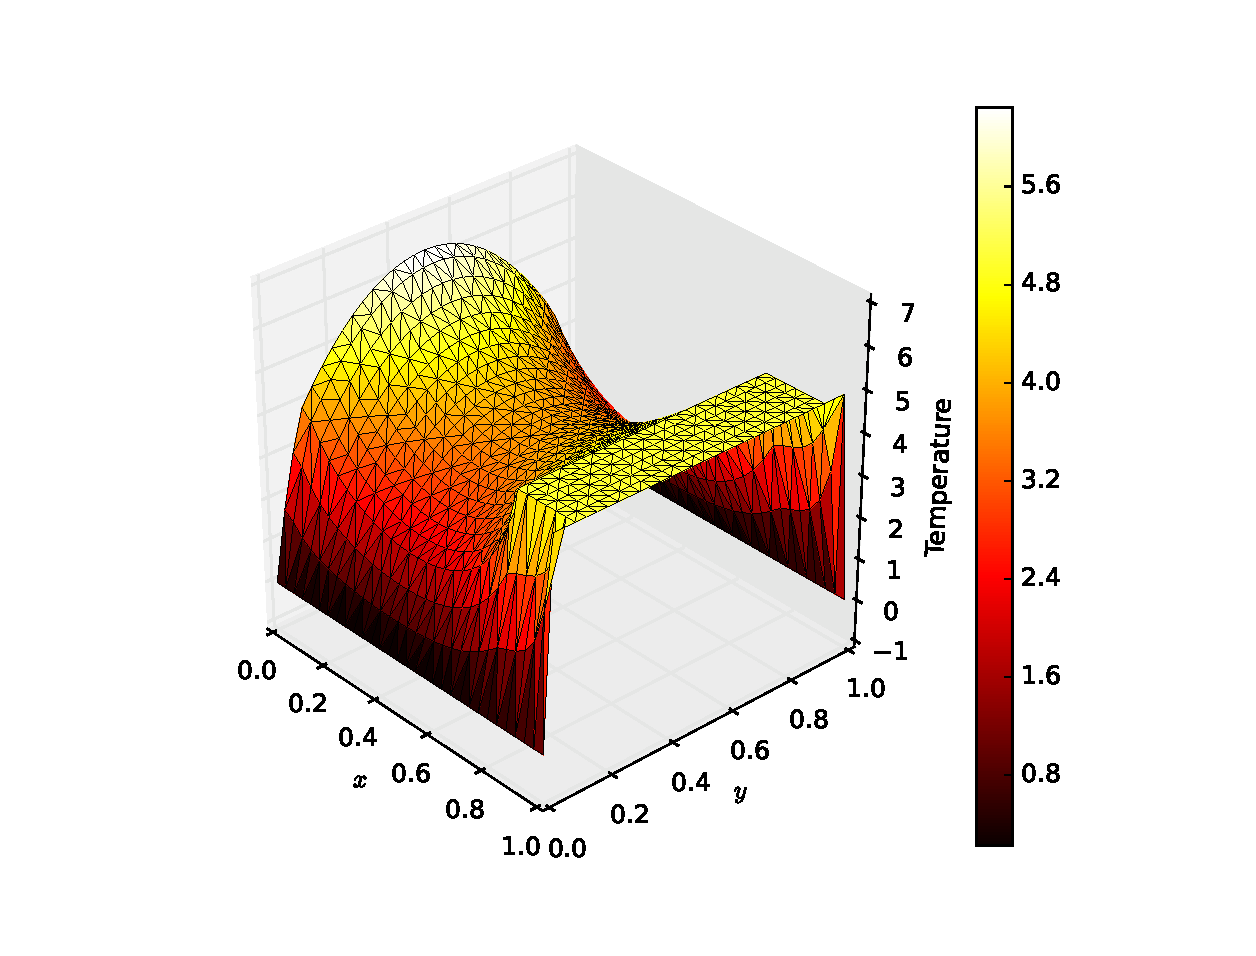
\includegraphics[width=1.2\textwidth]{fig/figure_6.eps}
		\caption{}
		\label{fig:1}
	\end{subfigure}
	\begin{subfigure}[H]{0.3\textwidth}
		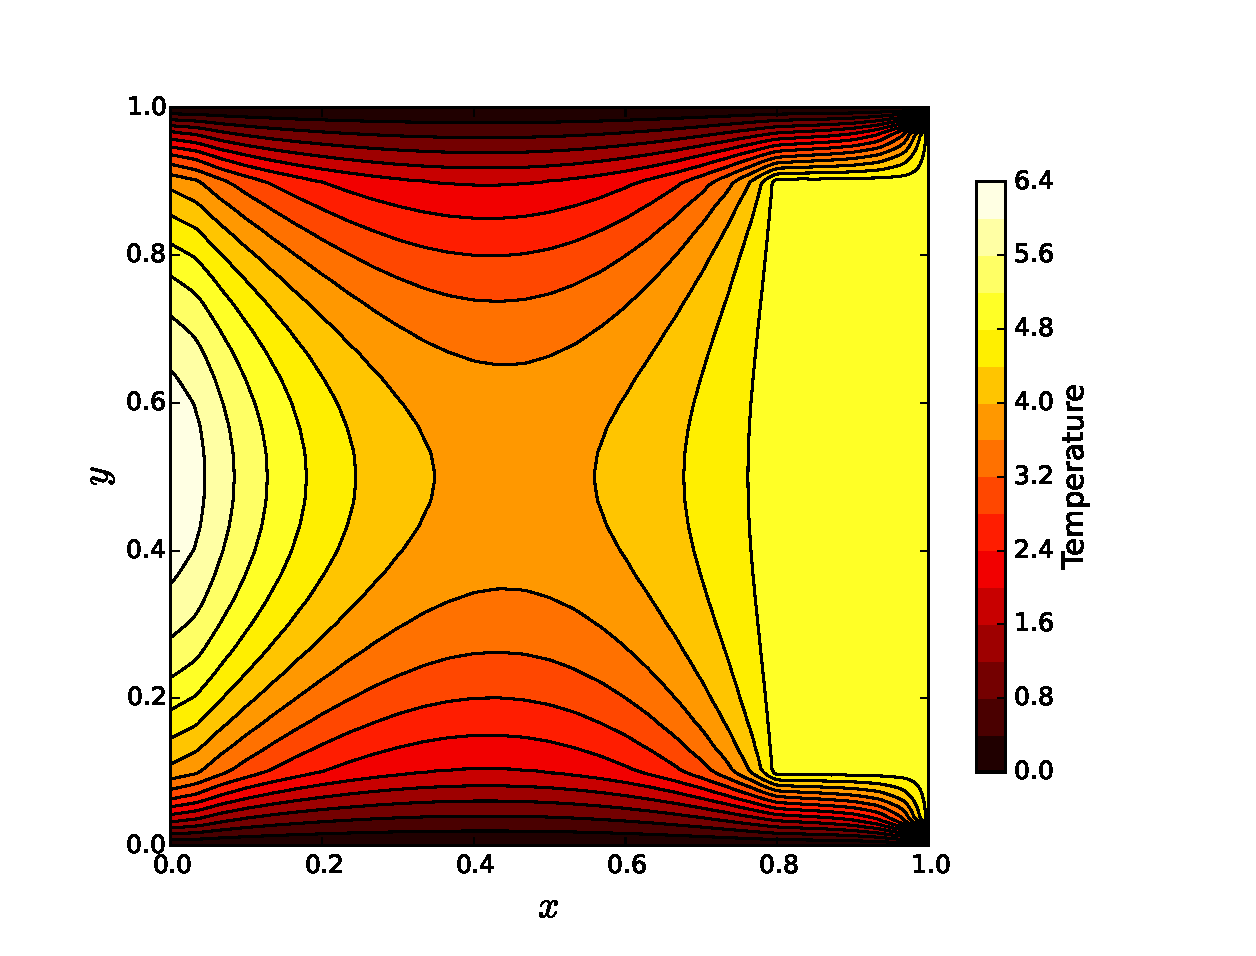
\includegraphics[width=\textwidth]{fig/figure_6.1.eps}
		\caption{}
		\label{fig:2}
	\end{subfigure}
	\caption{30 elements each direction}
	\label{fig:3_1}
\end{figure}

\begin{figure}[H]
\centering
	\begin{subfigure}[H]{0.3\textwidth}
		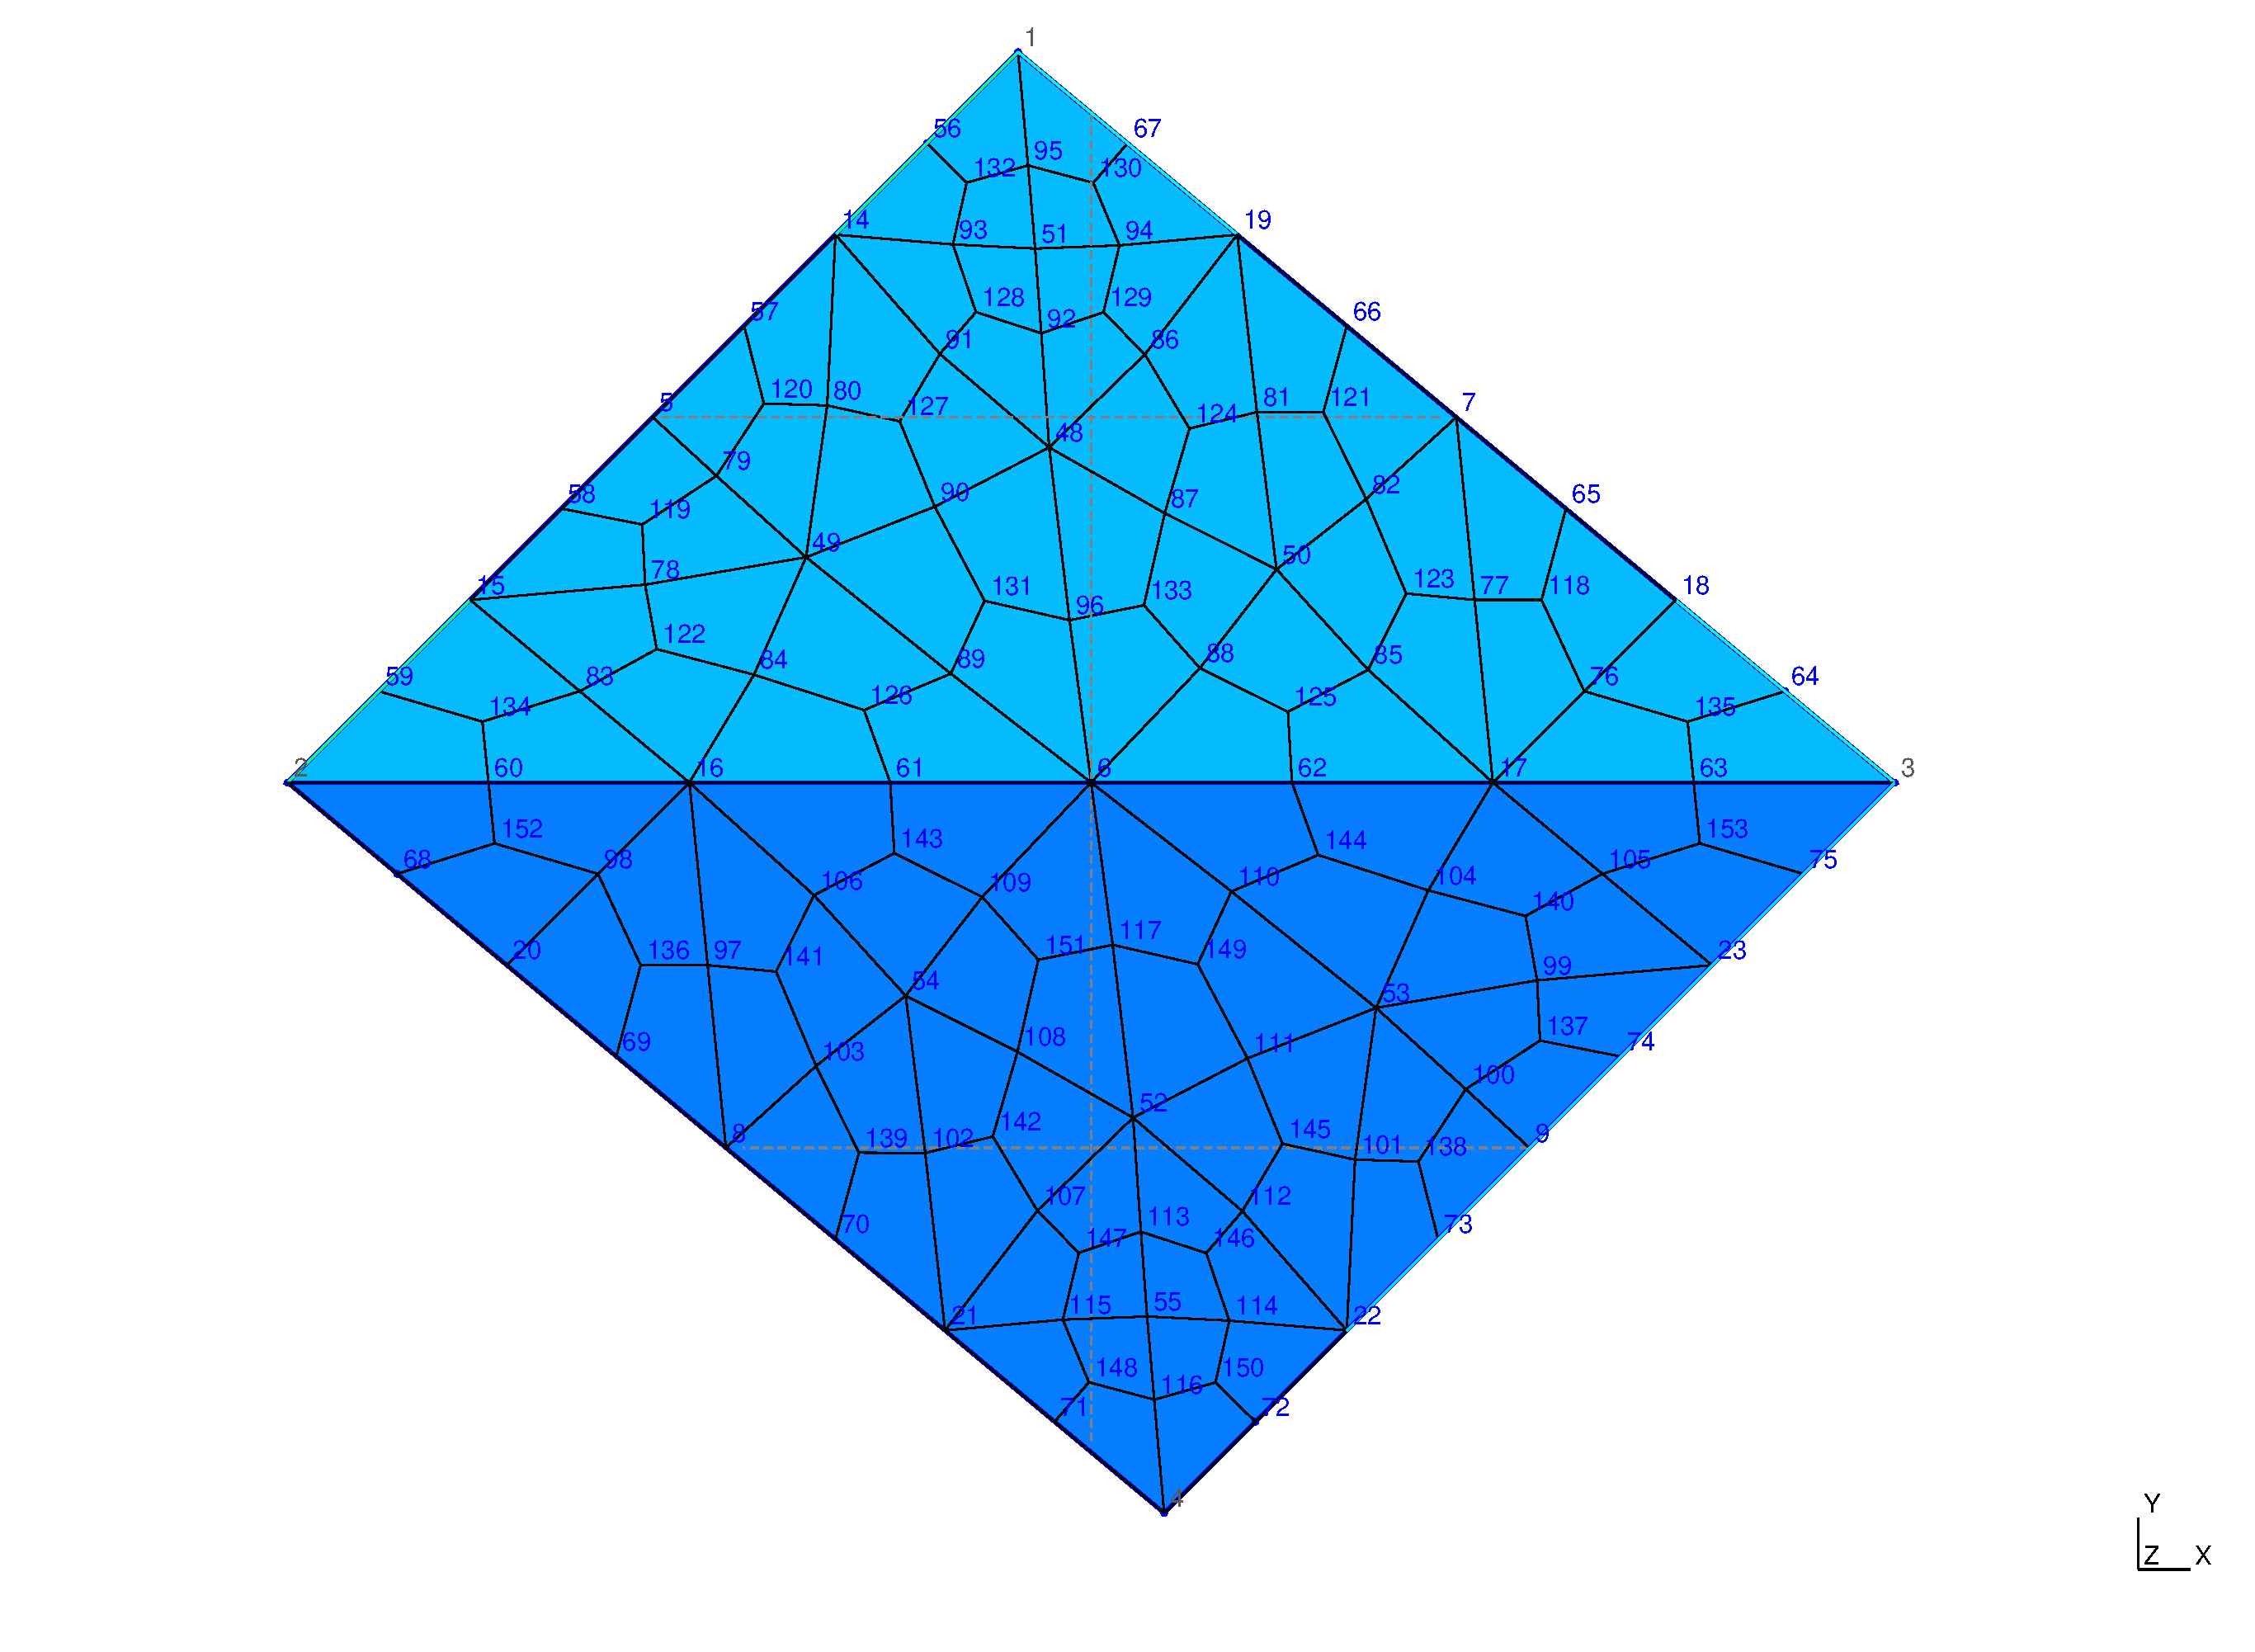
\includegraphics[width=1.2\textwidth]{fig/test2_1.eps}
		\caption{}
		\label{fig:1}
	\end{subfigure}
	\begin{subfigure}[H]{0.6\textwidth}
		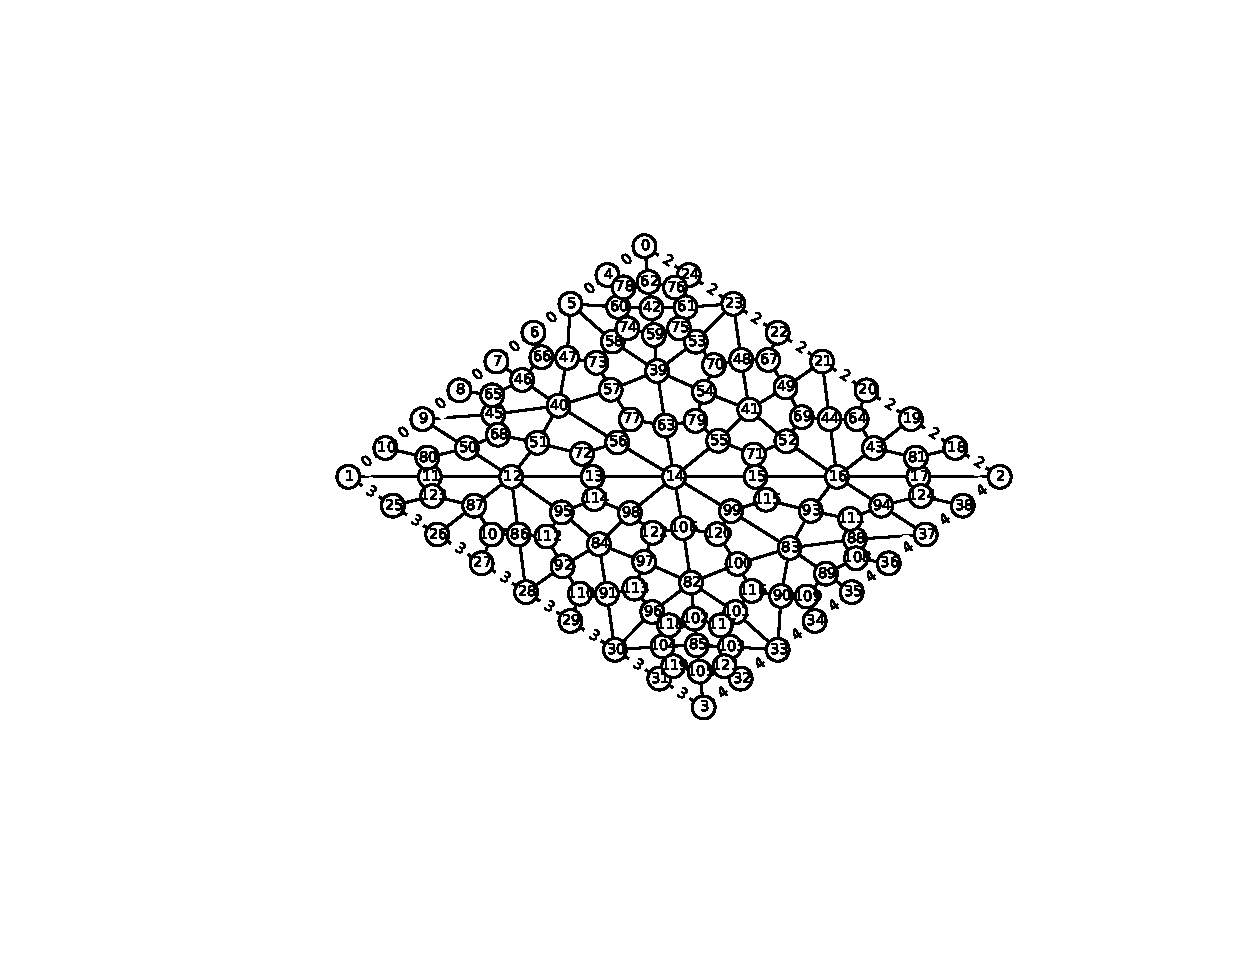
\includegraphics[width=\textwidth]{fig/test2_2.eps}
		\caption{}
		\label{fig:2}
	\end{subfigure}
	\begin{subfigure}[H]{0.45\textwidth}
		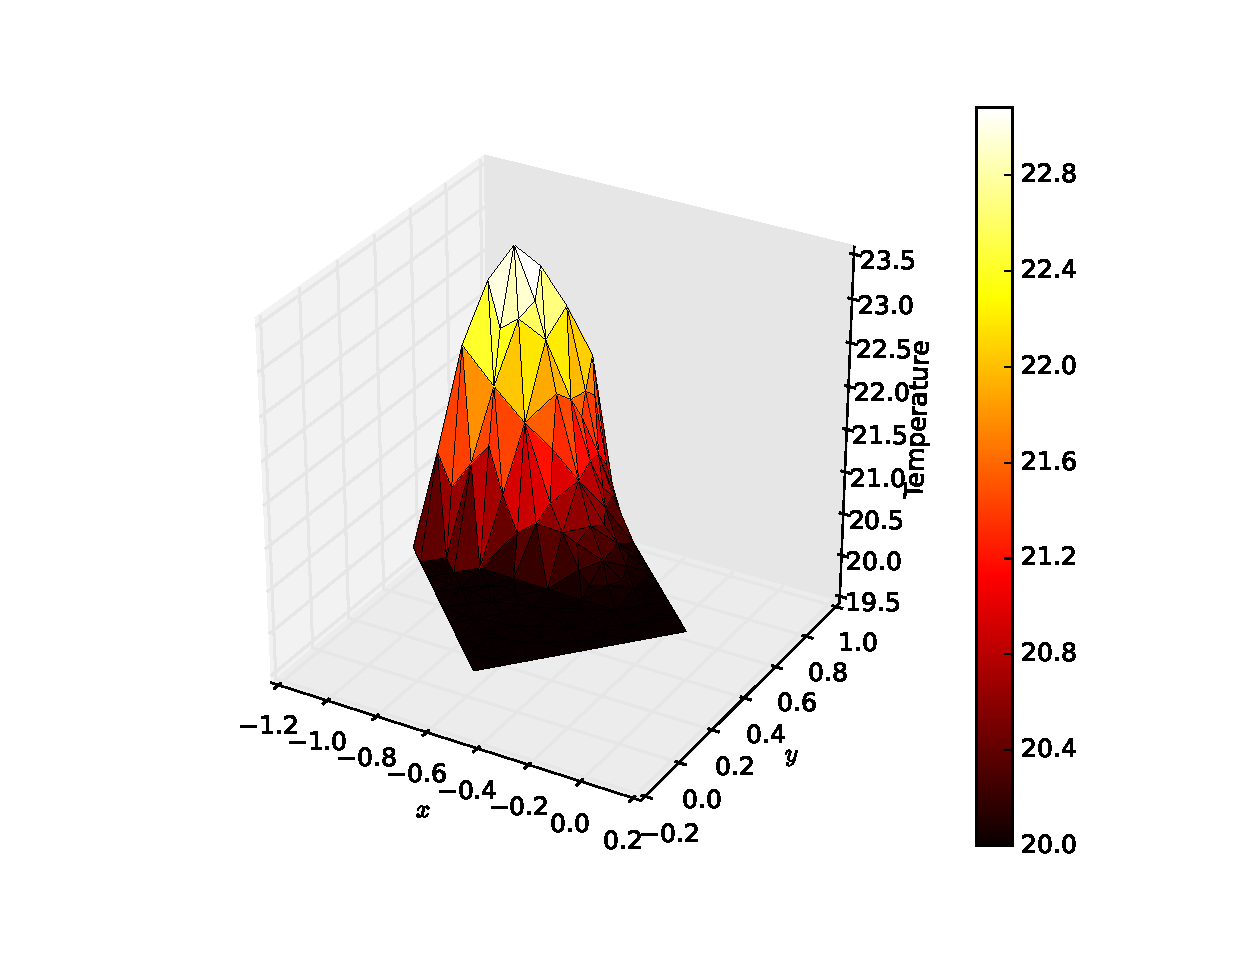
\includegraphics[width=\textwidth]{fig/test2_3.eps}
		\caption{}
		\label{fig:3}
	\end{subfigure}
	\begin{subfigure}[H]{0.45\textwidth}
		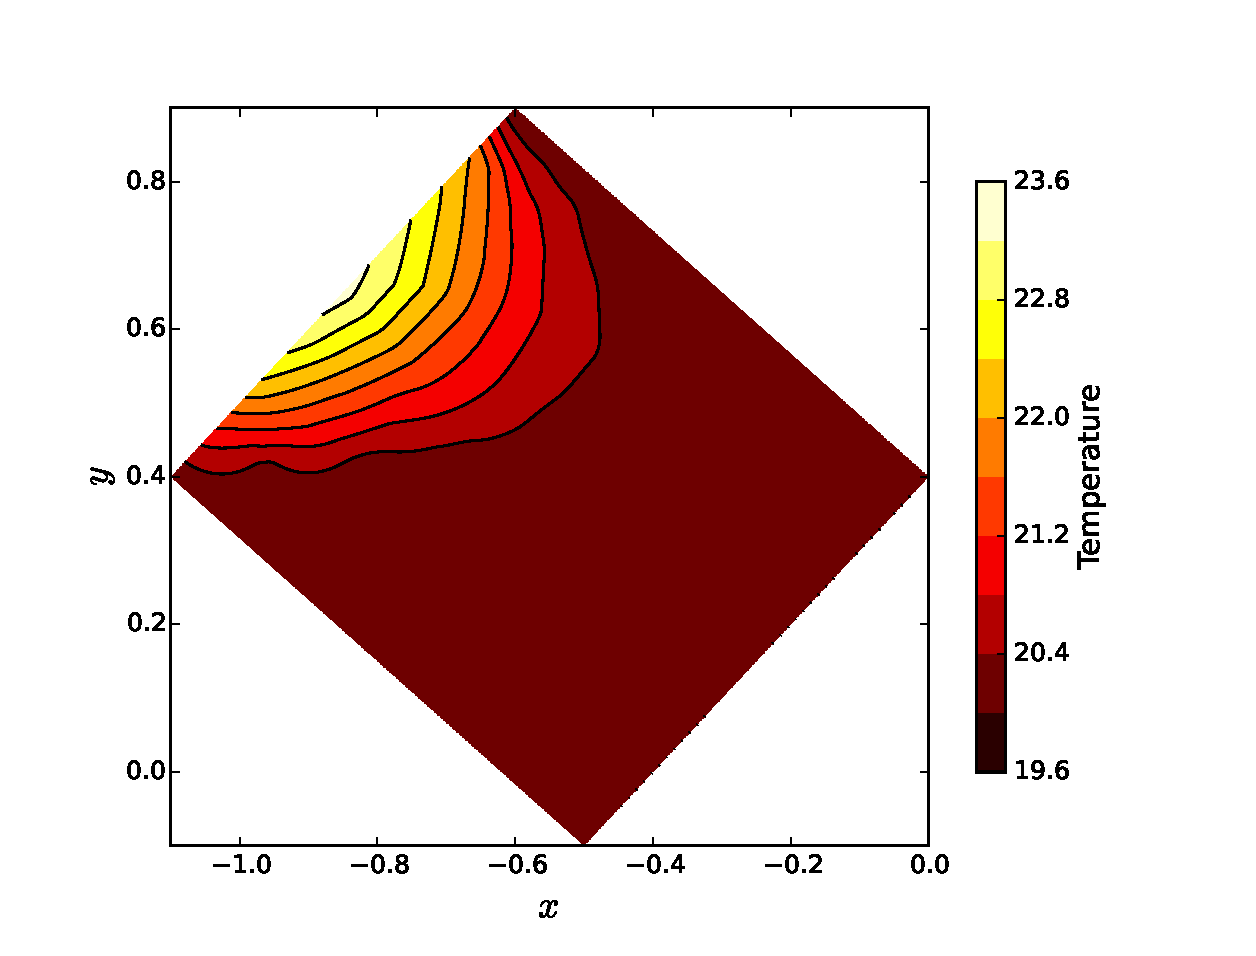
\includegraphics[width=\textwidth]{fig/test2_4.eps}
		\caption{}
		\label{fig:3}
	\end{subfigure}
	\caption{Internal load equals $q=0$, temperature k1 = 1 and k2= 1000.}
	\label{fig:3_1}
\end{figure}



\subsection{General Geometry}

\begin{figure}[H]
\centering
	\begin{subfigure}[H]{0.5\textwidth}
		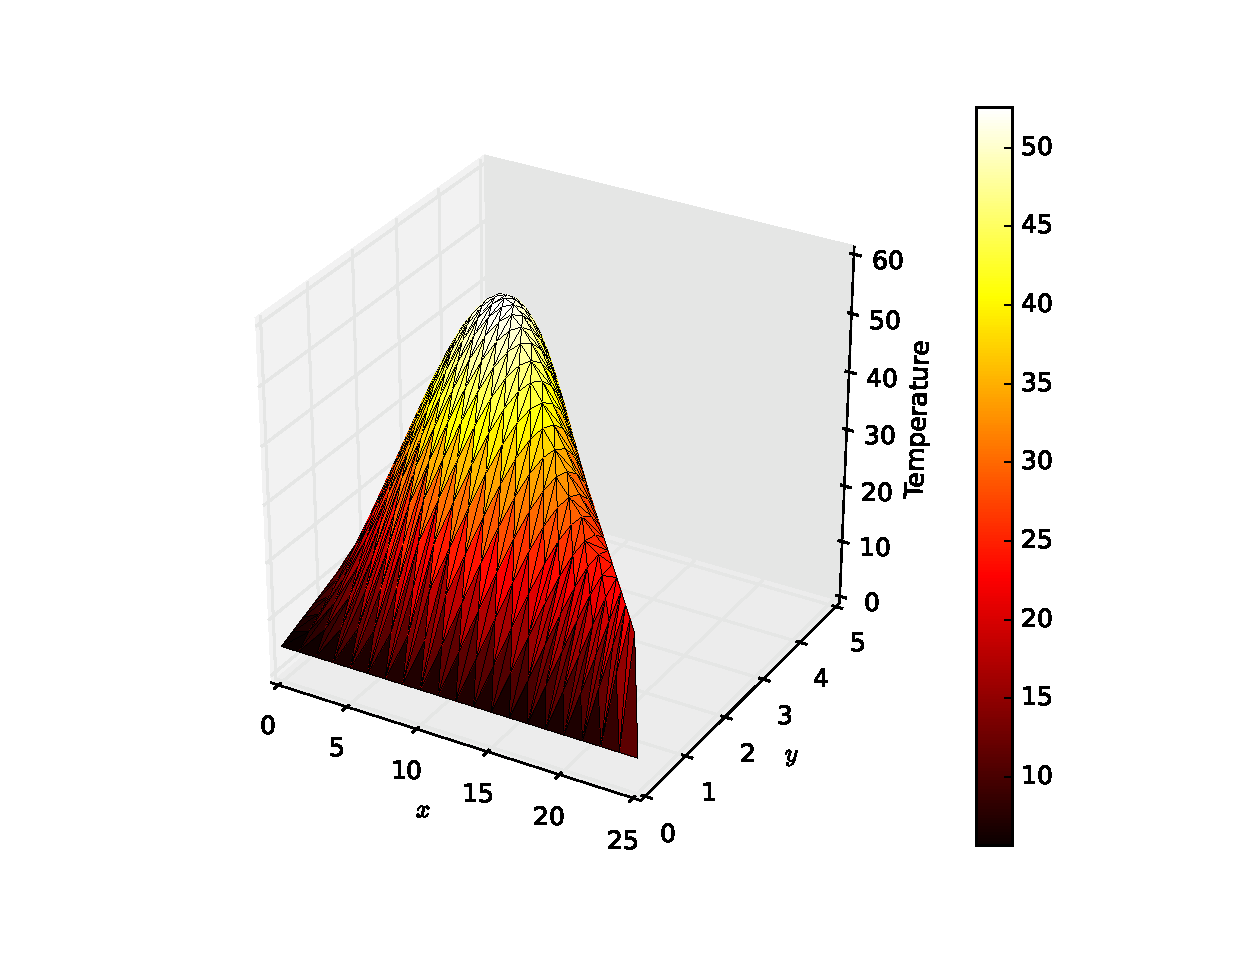
\includegraphics[width=1.2\textwidth]{fig/figure_7.eps}
		\caption{}
		\label{fig:1}
	\end{subfigure}
	\begin{subfigure}[H]{0.3\textwidth}
		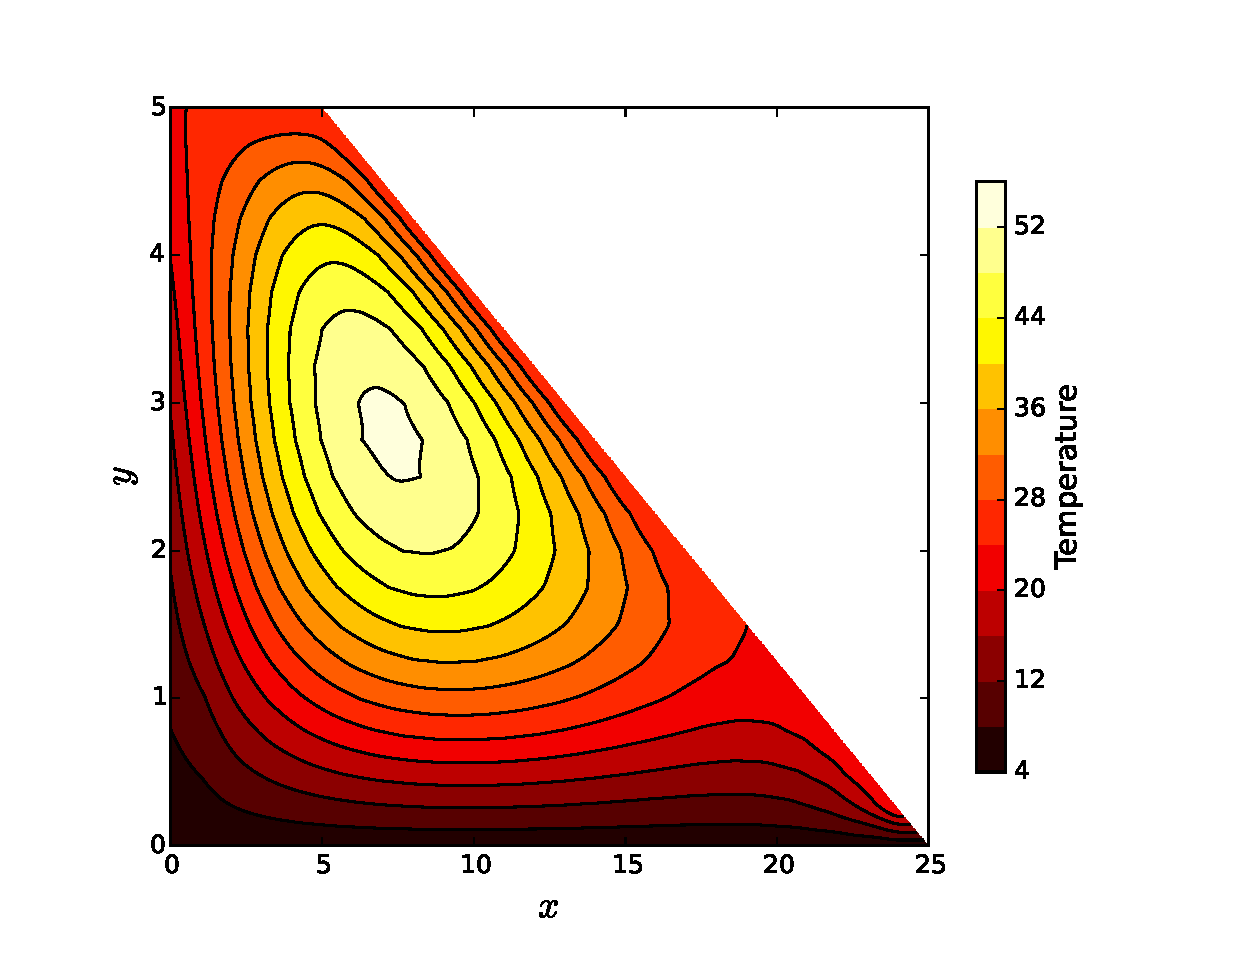
\includegraphics[width=\textwidth]{fig/figure_7.1.eps}
		\caption{}
		\label{fig:2}
	\end{subfigure}
	\caption{20 elements, internal source $q=x_1 x_2$ and linear temperature distribution on the left side}
	\label{fig:3_1}
\end{figure}


\begin{figure}[H]
\centering
	\begin{subfigure}[H]{0.3\textwidth}
		\includegraphics[width=1.2\textwidth]{fig/test1_1.eps}
		\caption{}
		\label{fig:1}
	\end{subfigure}
	\begin{subfigure}[H]{0.33\textwidth}
		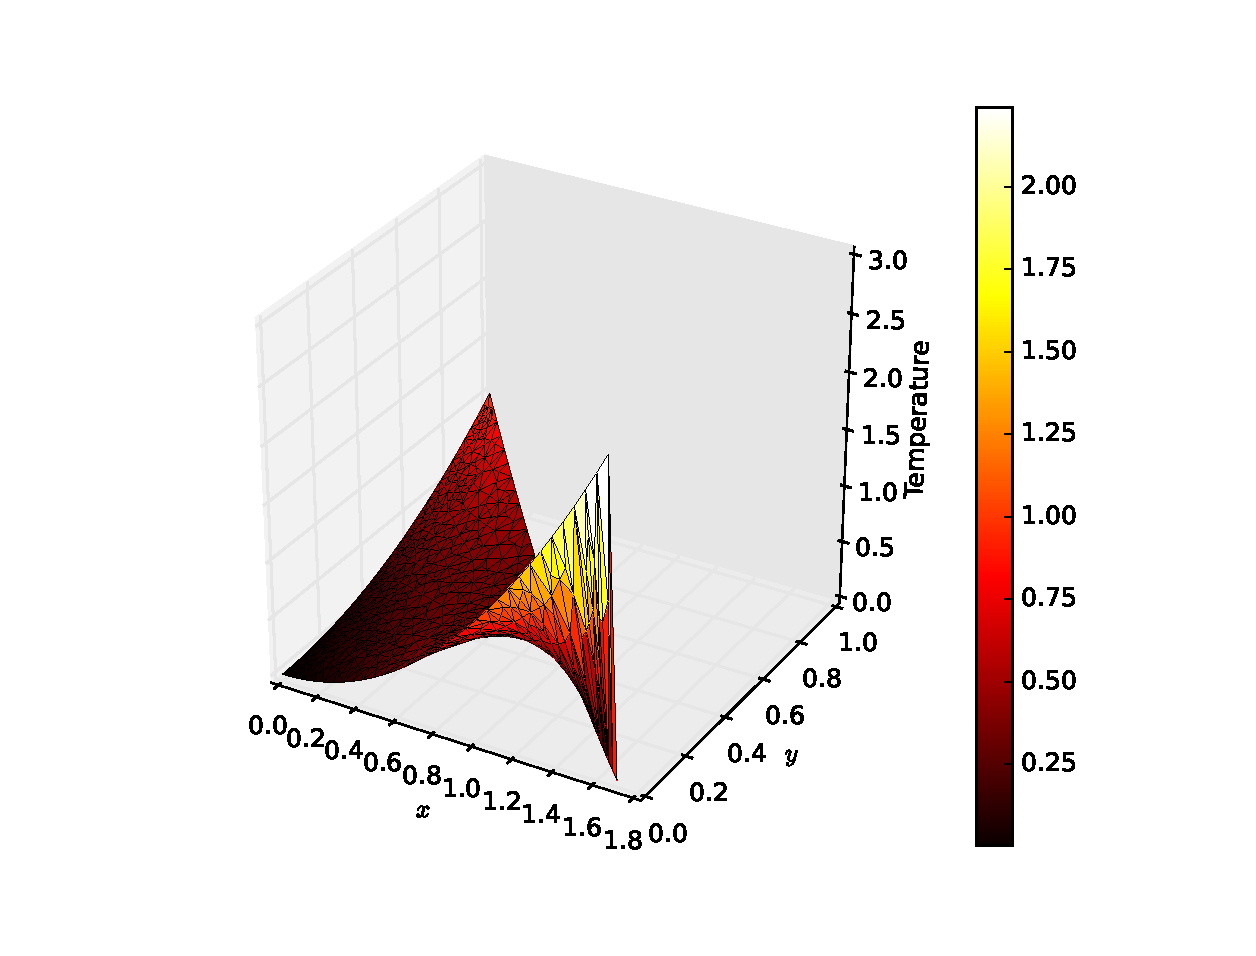
\includegraphics[width=\textwidth]{fig/test1_2.eps}
		\caption{}
		\label{fig:2}
	\end{subfigure}
	\begin{subfigure}[H]{0.33\textwidth}
		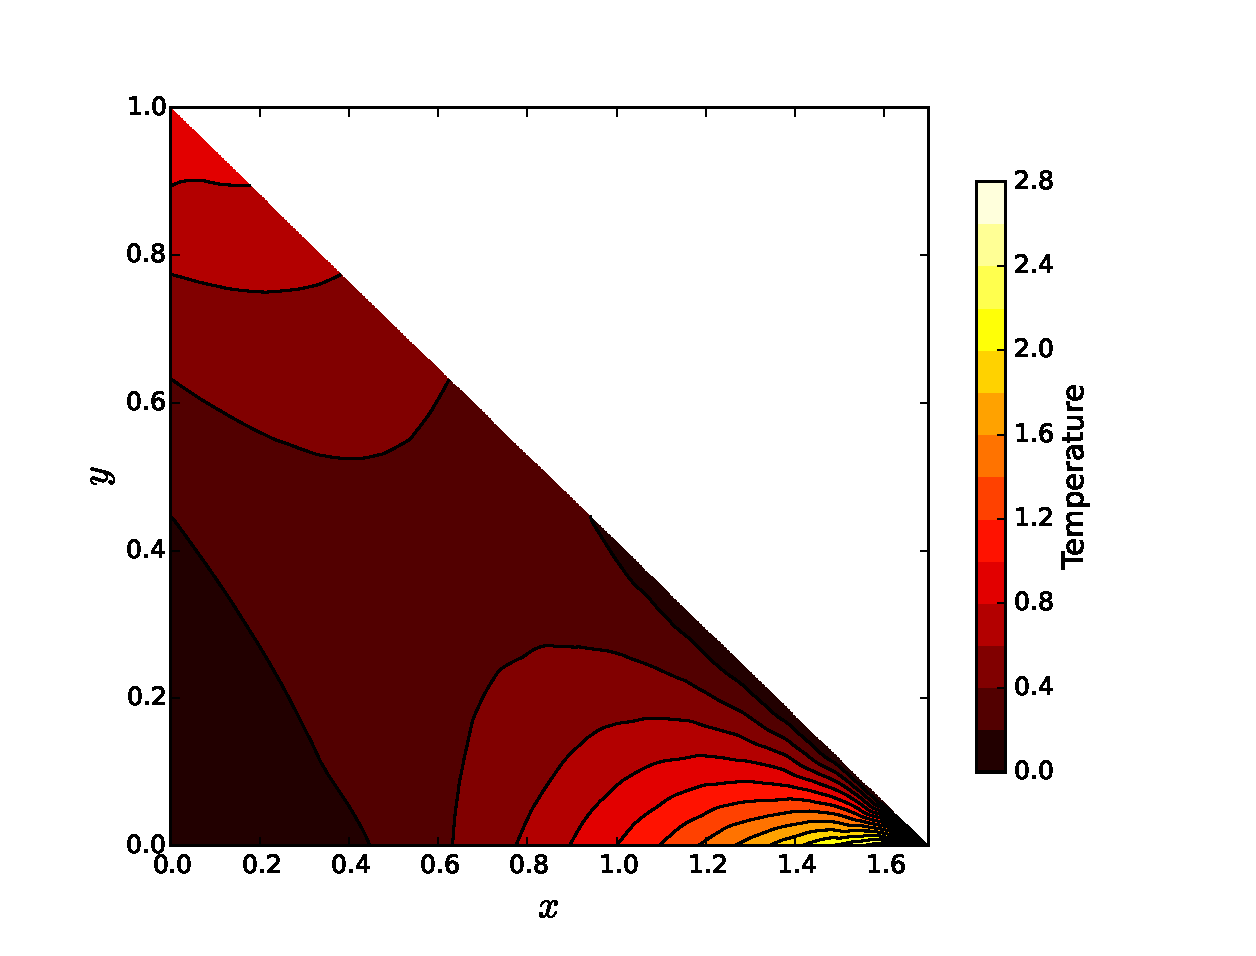
\includegraphics[width=\textwidth]{fig/test1_3.eps}
		\caption{}
		\label{fig:3}
	\end{subfigure}
	\caption{Internal load equals $q=x_1^2/10 + x_2^2/10$, temperature on the sides starts at the bottom and goes ccw $T=[x_1^2, x_2^2, x_2^2]$.}
	\label{fig:3_1}
\end{figure}


\subsection{Dam Examples}


\begin{figure}[H]
\centering
	\begin{subfigure}[H]{0.3\textwidth}
		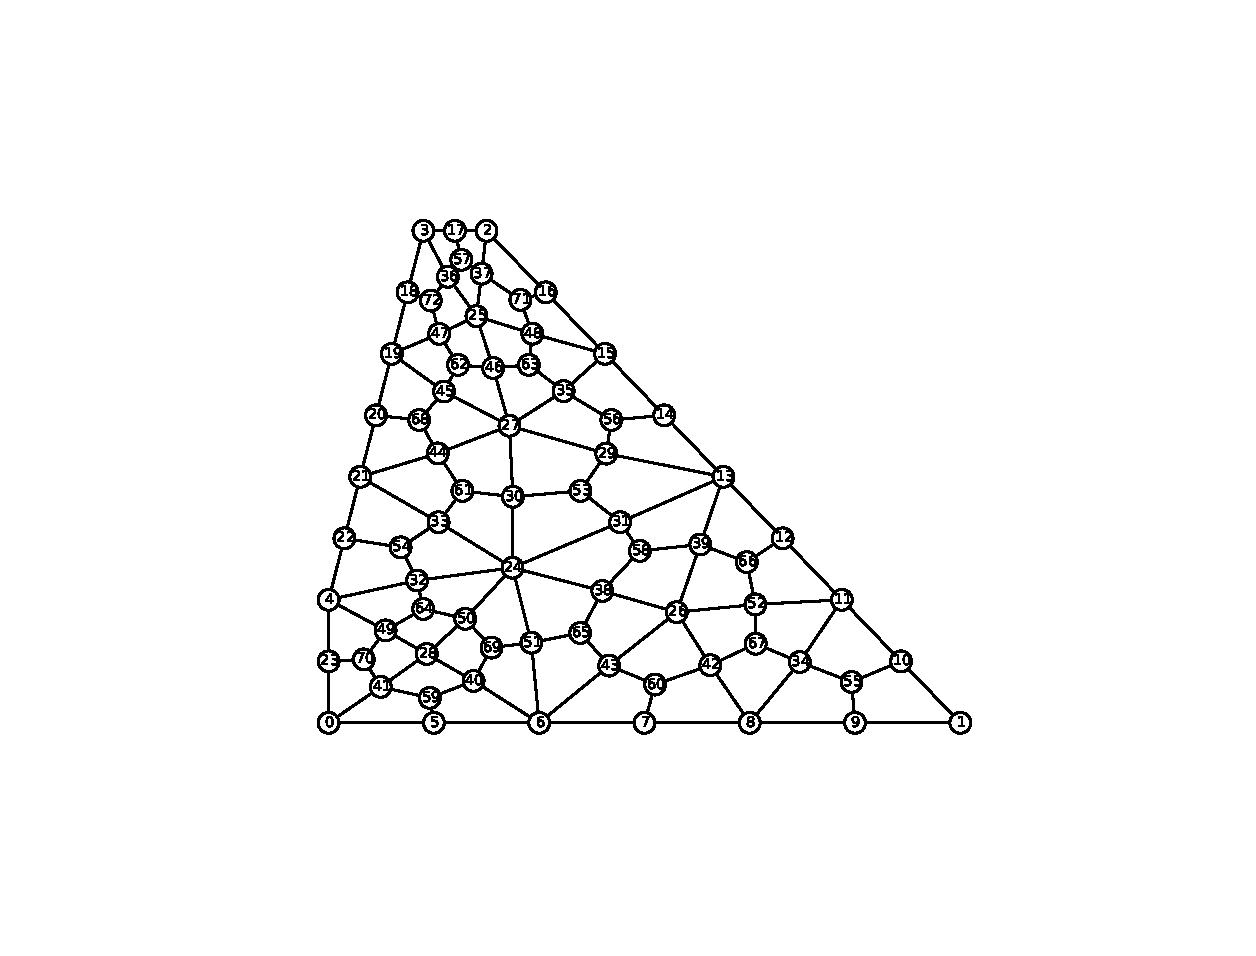
\includegraphics[width=1.2\textwidth]{fig/exdam1_1.eps}
		\caption{}
		\label{fig:1}
	\end{subfigure}
	\begin{subfigure}[H]{0.33\textwidth}
		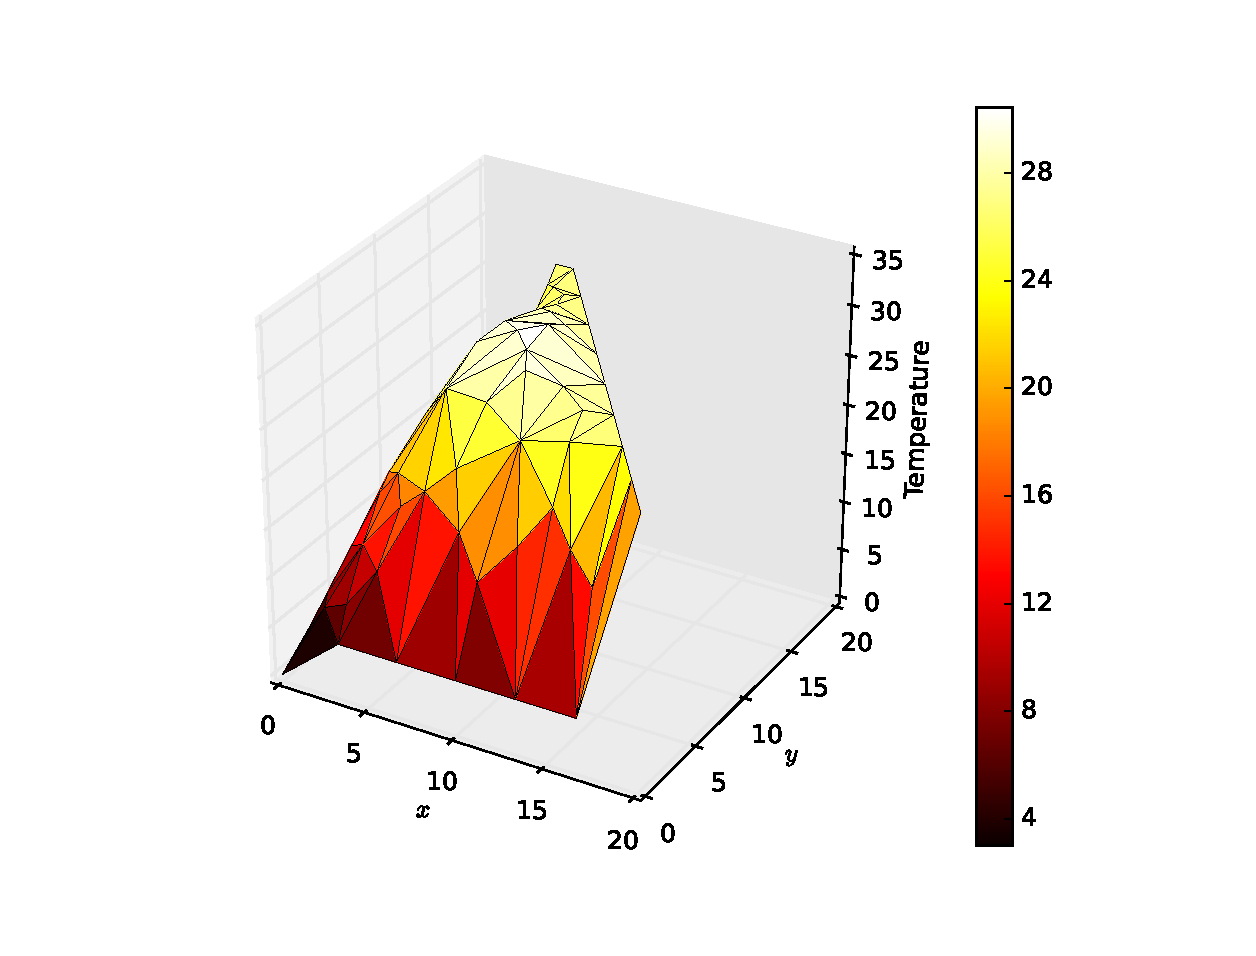
\includegraphics[width=\textwidth]{fig/exdam1_2.eps}
		\caption{}
		\label{fig:2}
	\end{subfigure}
	\begin{subfigure}[H]{0.33\textwidth}
		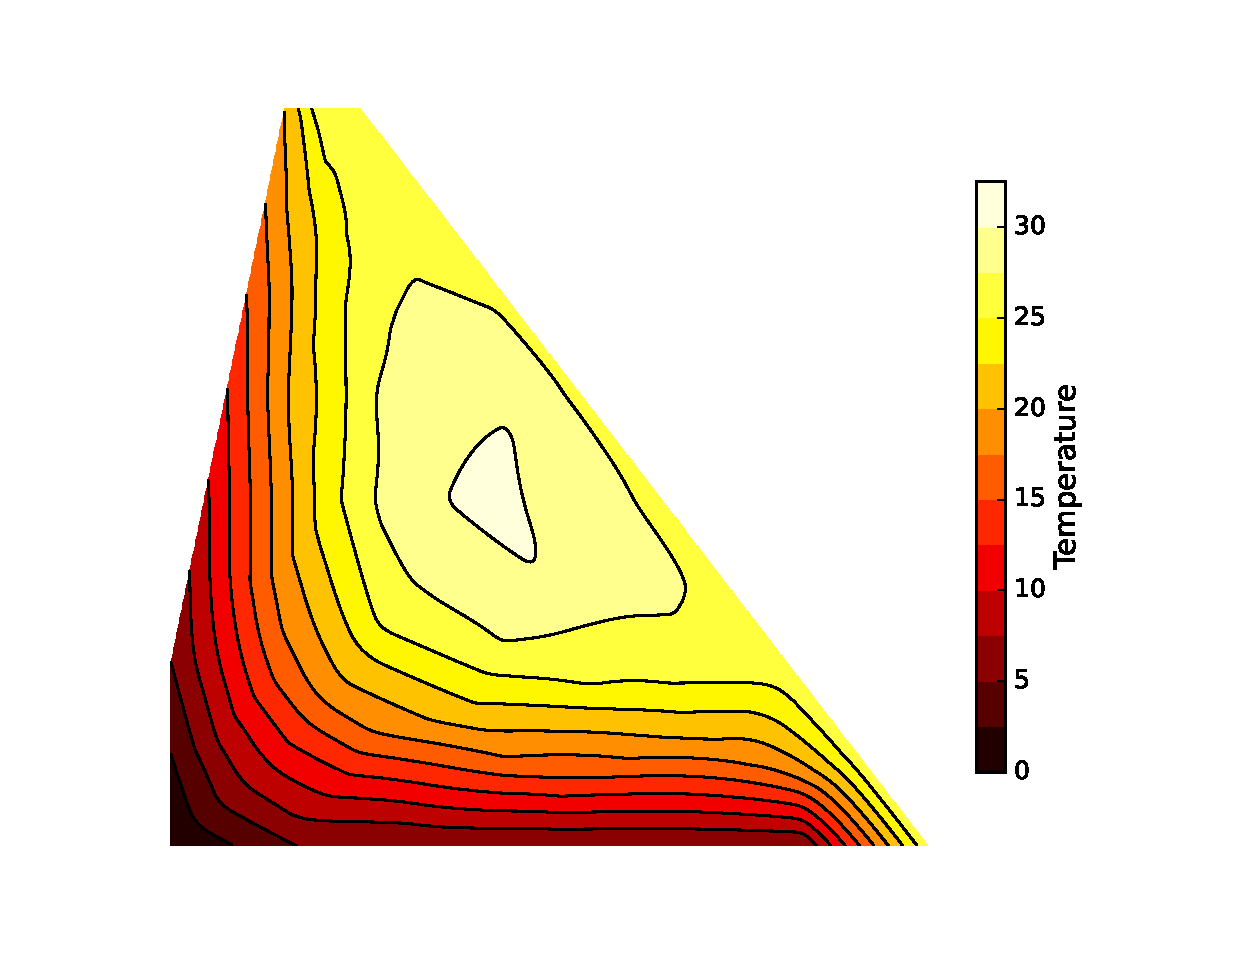
\includegraphics[width=\textwidth]{fig/exdam1_3.eps}
		\caption{}
		\label{fig:3}
	\end{subfigure}
	\caption{Internal load equals $q=1$, temperature on the sides starts at the bottom and goes ccw $T=[5, 27, 27, x2, x2]$.}
	\label{fig:3_1}
\end{figure}


\begin{figure}[H]
\centering
	\begin{subfigure}[H]{0.3\textwidth}
		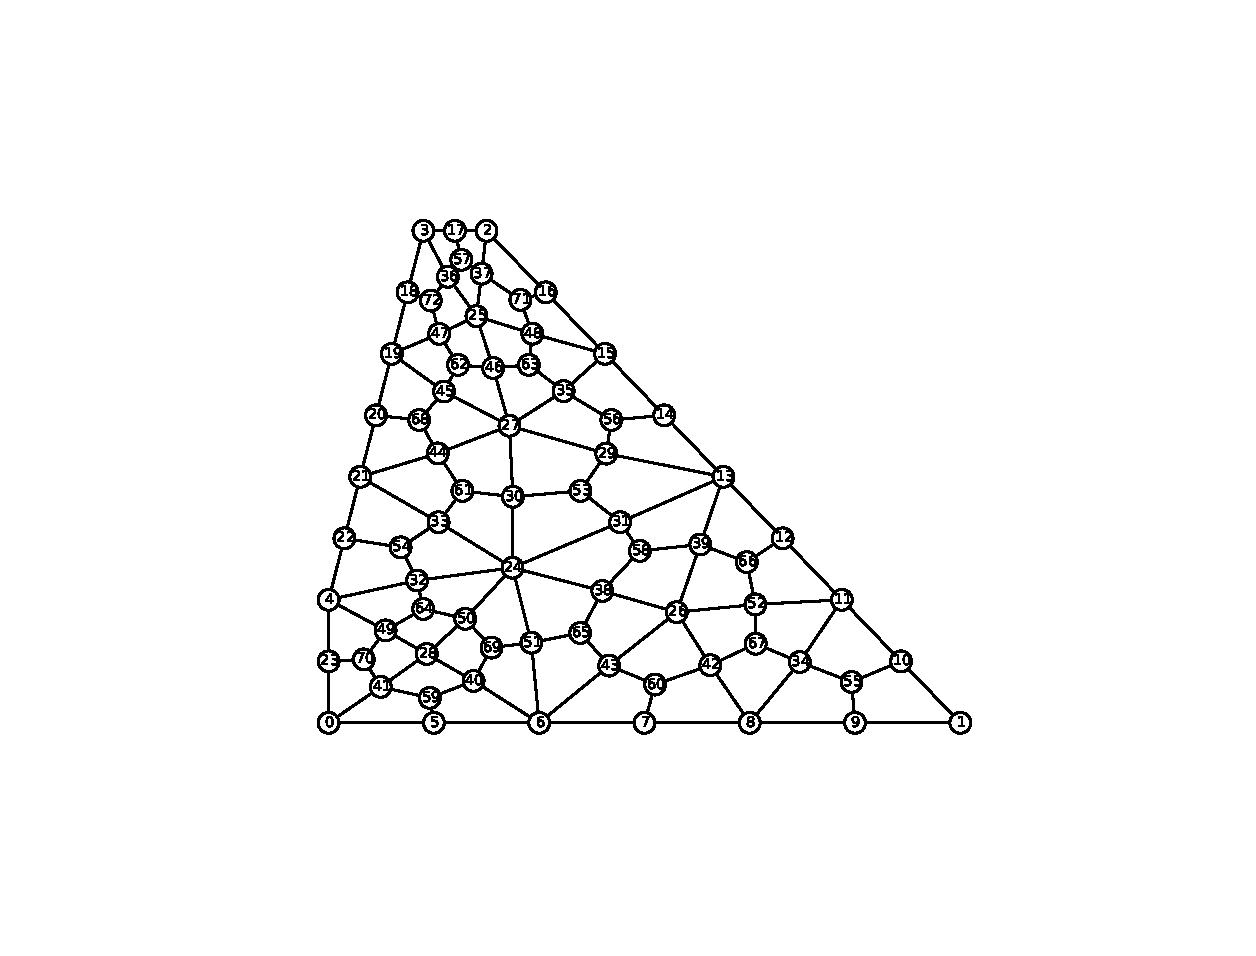
\includegraphics[width=1.2\textwidth]{fig/exdam2_1.eps}
		\caption{}
		\label{fig:1}
	\end{subfigure}
	\begin{subfigure}[H]{0.33\textwidth}
		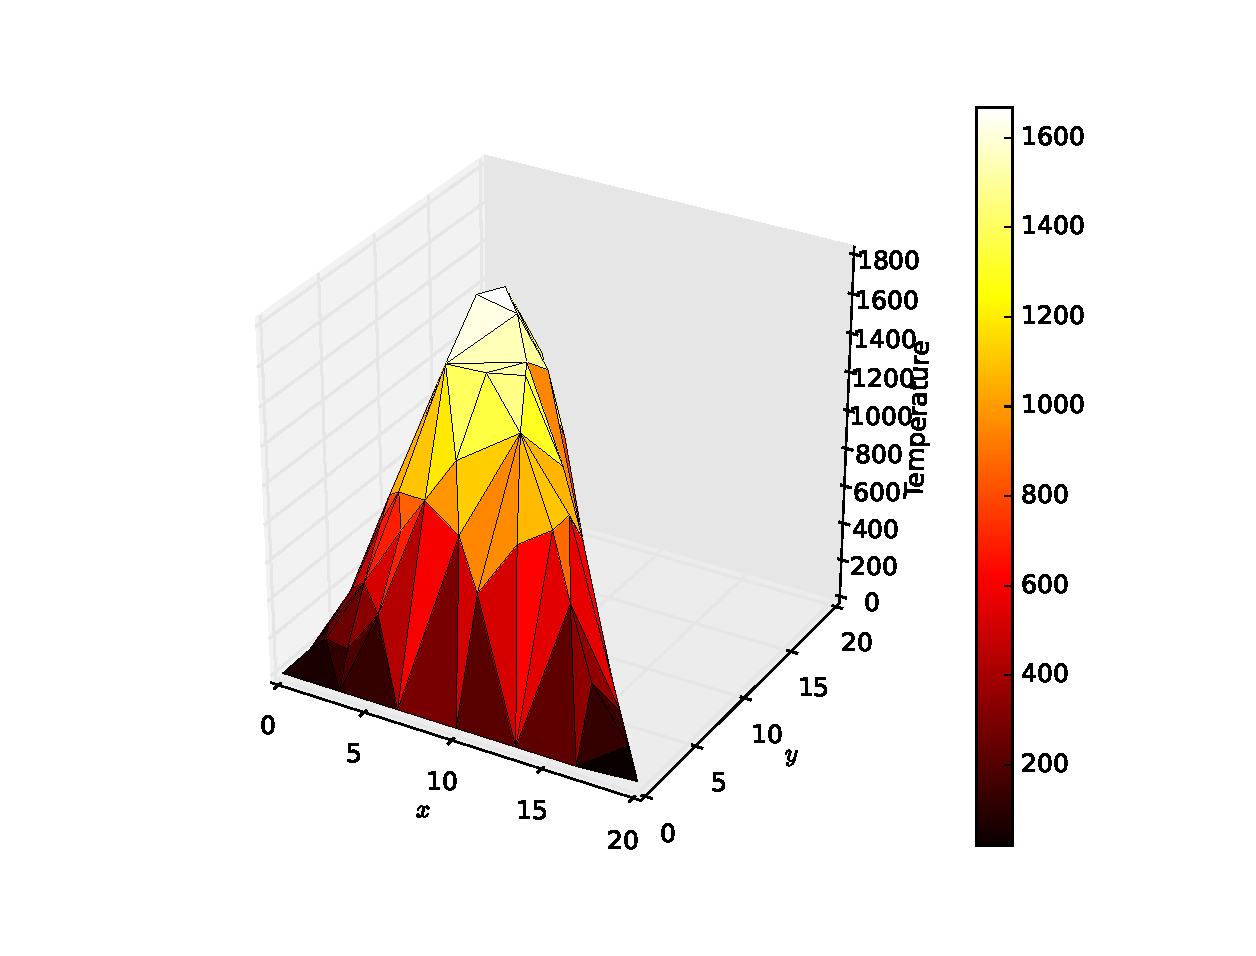
\includegraphics[width=\textwidth]{fig/exdam2_2.eps}
		\caption{}
		\label{fig:2}
	\end{subfigure}
	\begin{subfigure}[H]{0.33\textwidth}
		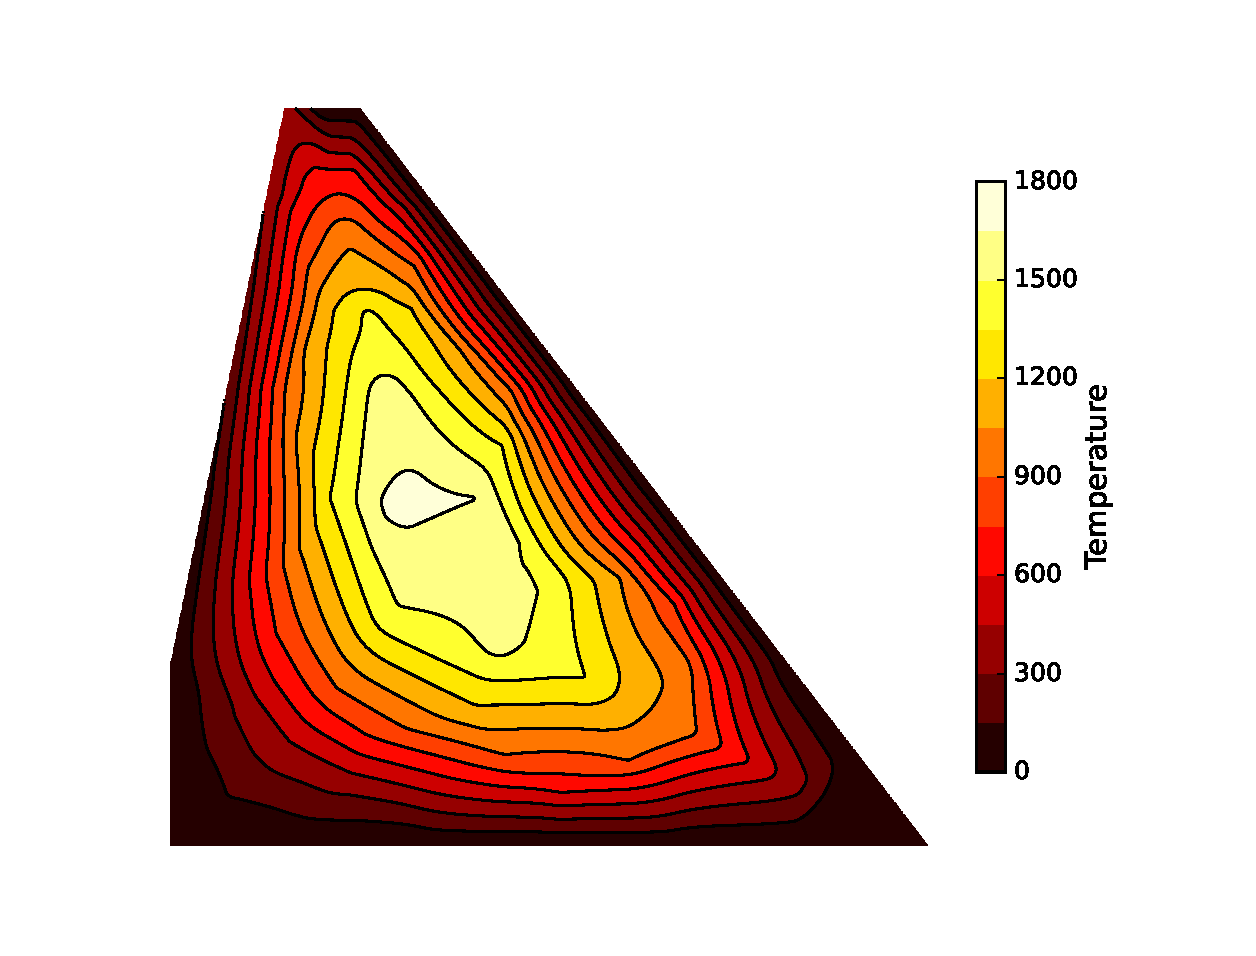
\includegraphics[width=\textwidth]{fig/exdam2_3.eps}
		\caption{}
		\label{fig:3}
	\end{subfigure}
	\caption{Internal load equals $q=x_1^2 + x_2^2$, temperature on the sides starts at the bottom and goes ccw $T=[5, 27, 27, x2, x2+5]$.}
	\label{fig:3_1}
\end{figure}



\begin{figure}[H]
\centering
	\begin{subfigure}[H]{0.3\textwidth}
		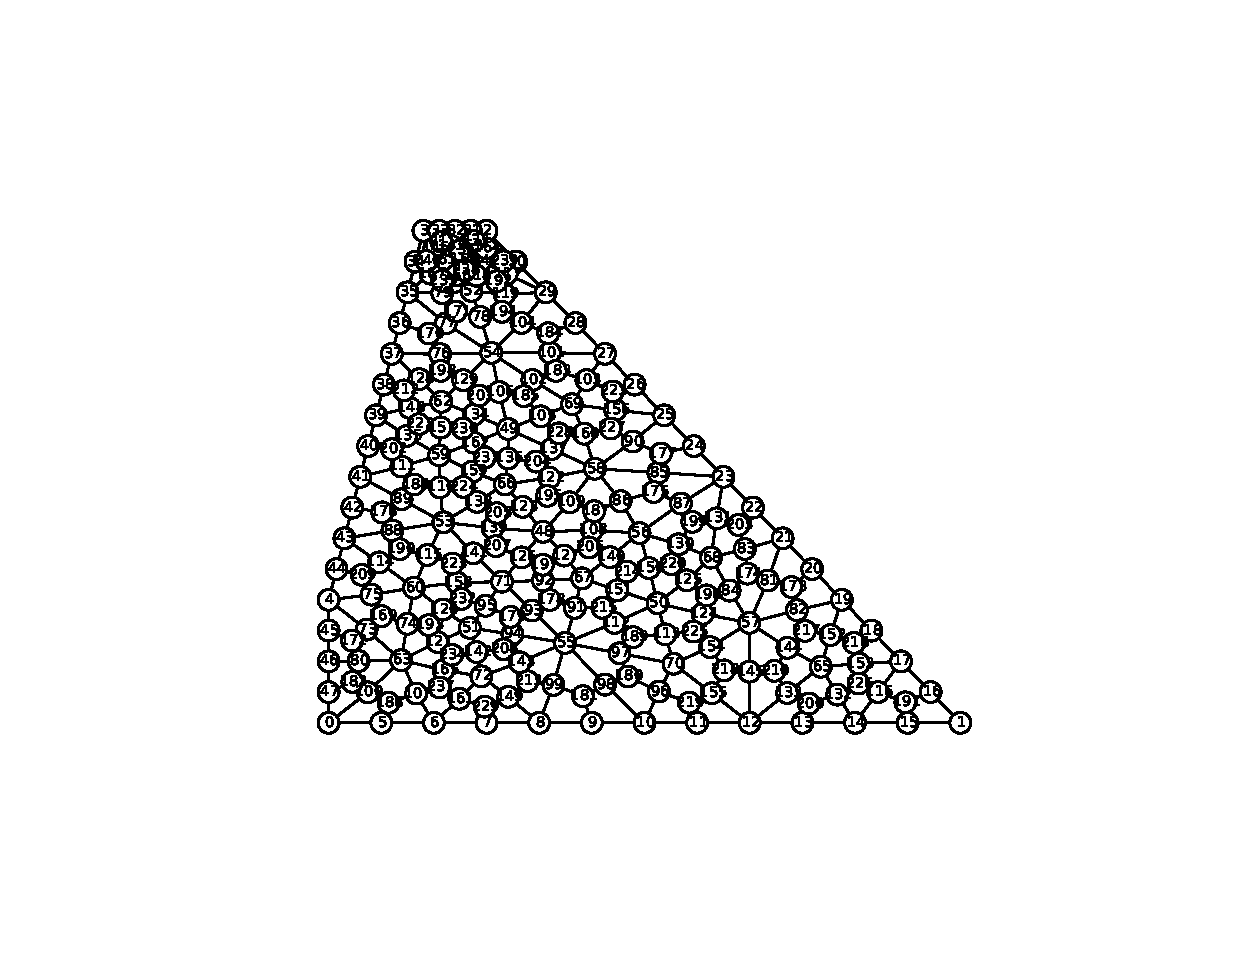
\includegraphics[width=1.2\textwidth]{fig/exdam3_1.eps}
		\caption{}
		\label{fig:1}
	\end{subfigure}
	\begin{subfigure}[H]{0.33\textwidth}
		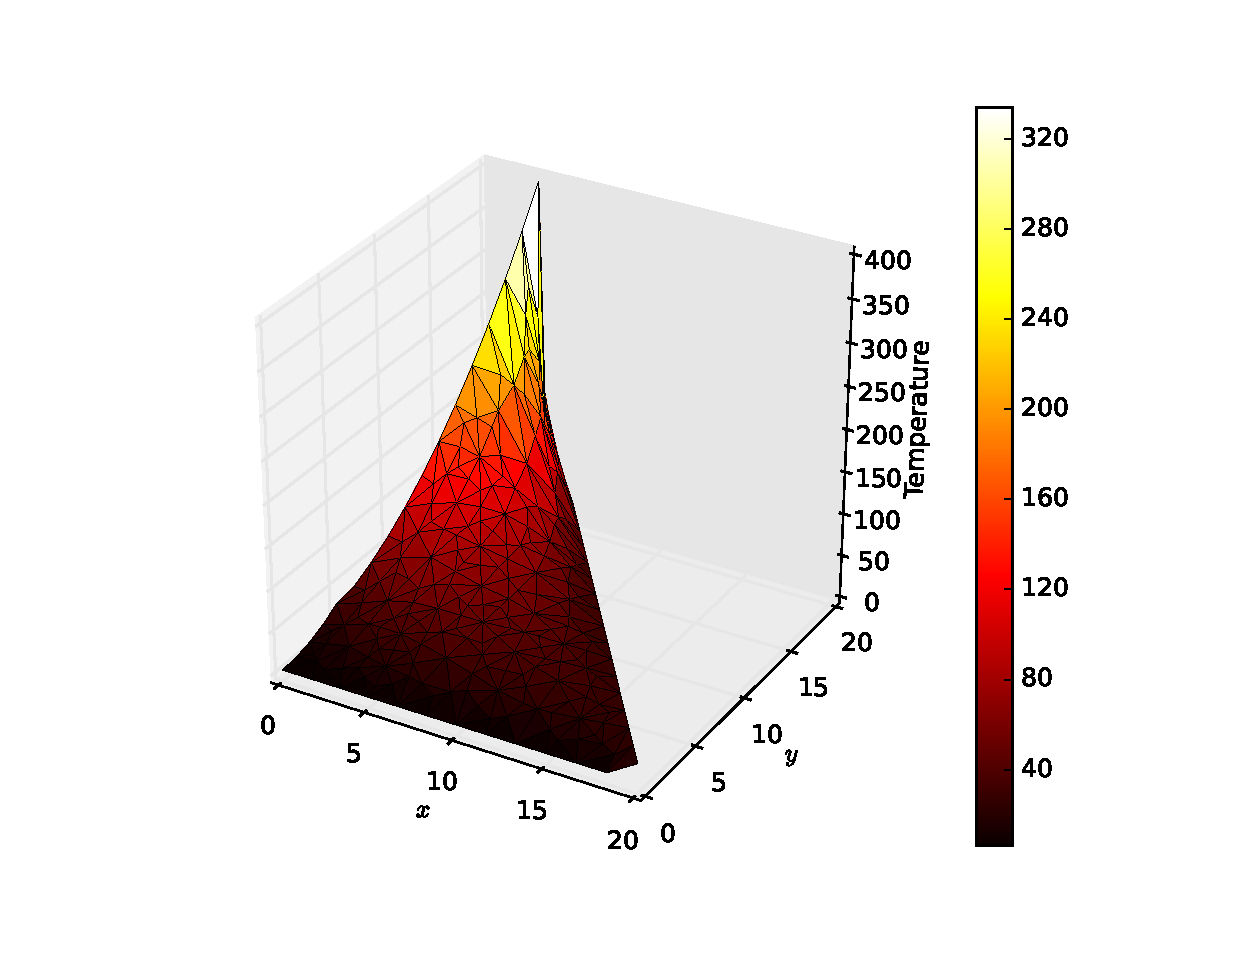
\includegraphics[width=\textwidth]{fig/exdam3_2.eps}
		\caption{}
		\label{fig:2}
	\end{subfigure}
	\begin{subfigure}[H]{0.33\textwidth}
		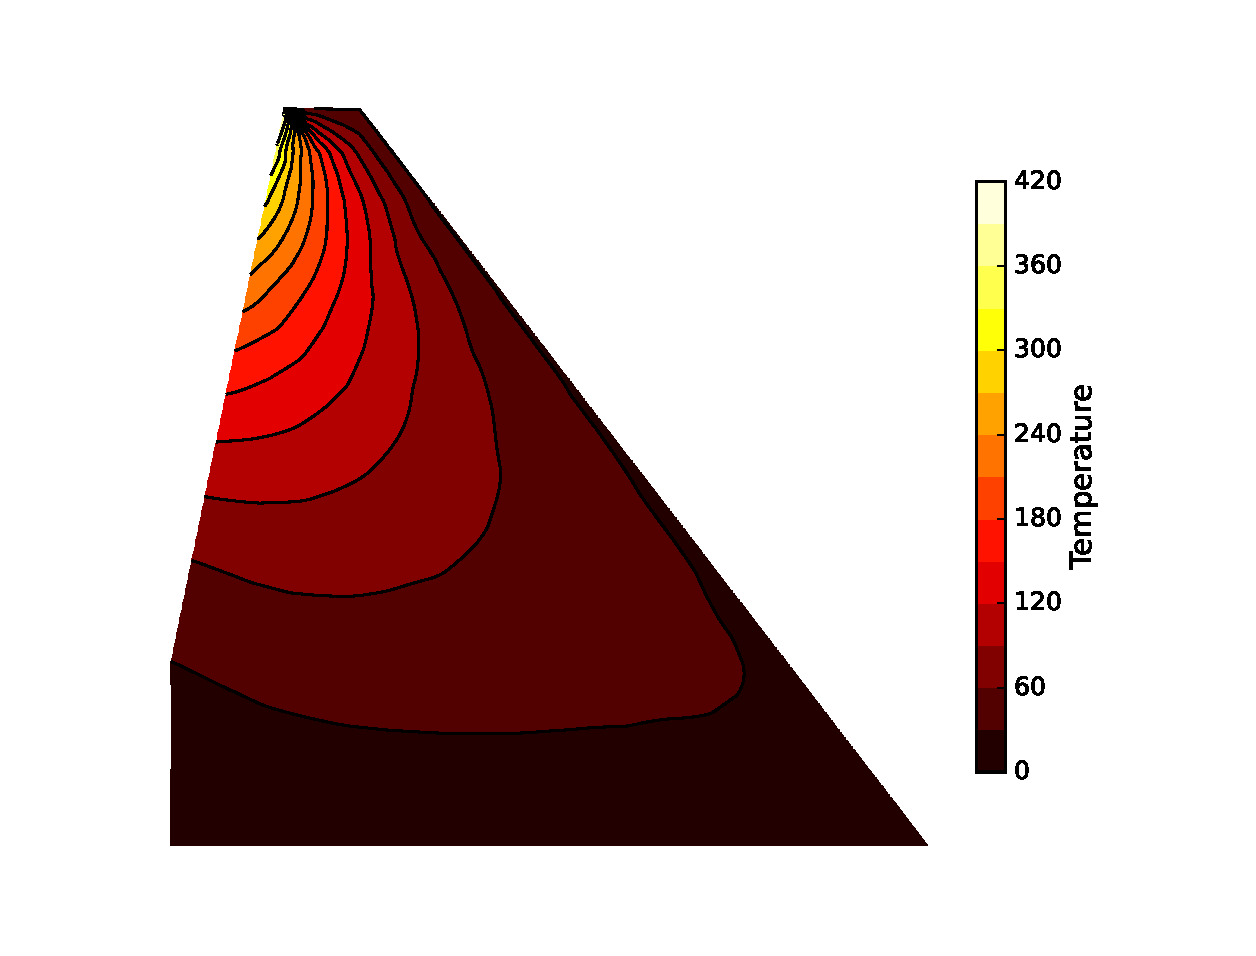
\includegraphics[width=\textwidth]{fig/exdam3_3.eps}
		\caption{}
		\label{fig:3}
	\end{subfigure}
	\caption{Internal load equals $q=x_1^2/10 + x_2^2/10$, temperature on the sides starts at the bottom and goes ccw $T=[5, 27, 27, x2^2, x2^2+5]$.}
	\label{fig:3_1}
\end{figure}


\begin{figure}[H]
\centering
	\begin{subfigure}[H]{0.3\textwidth}
		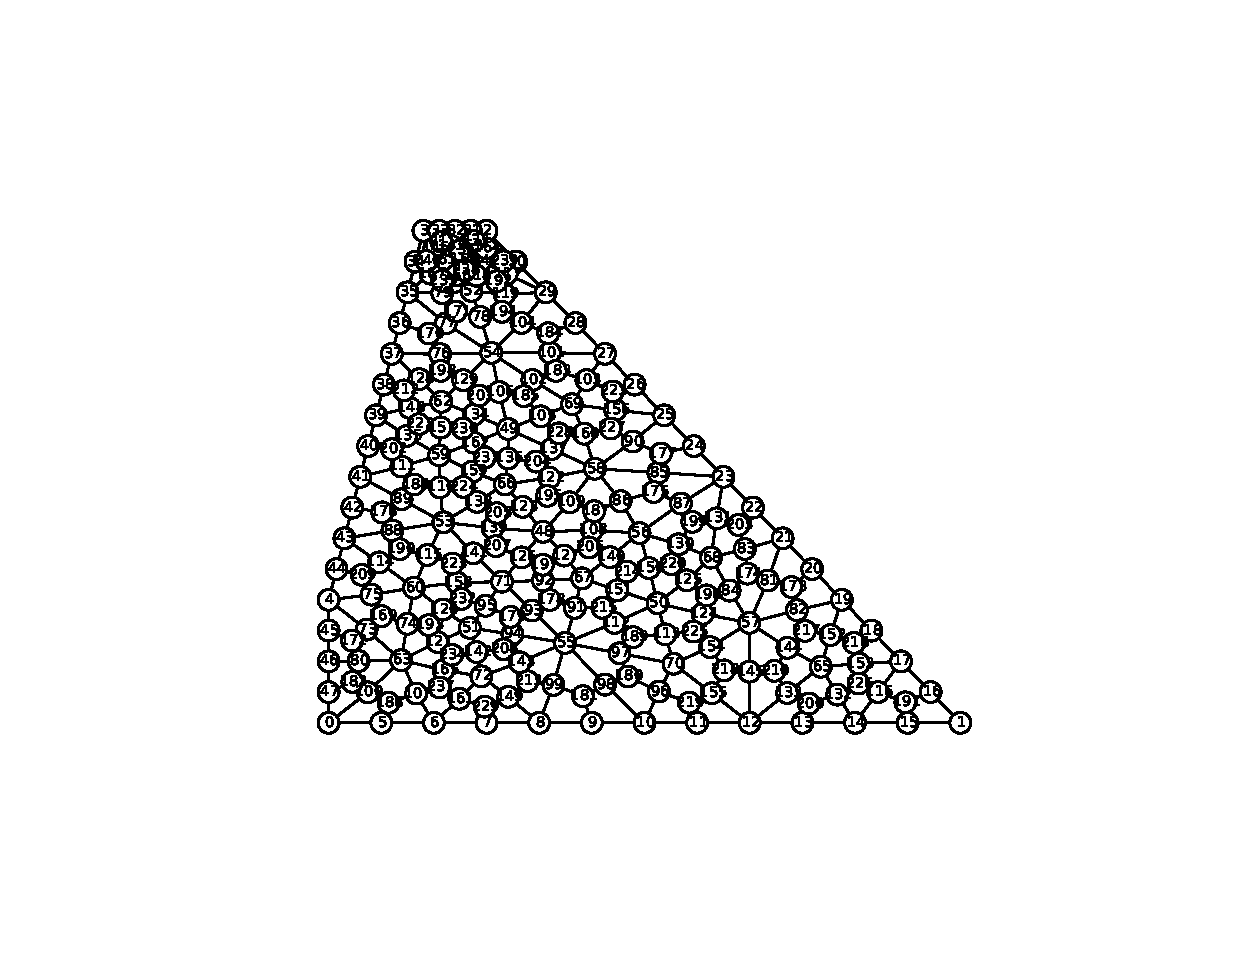
\includegraphics[width=1.2\textwidth]{fig/exdam4_1.eps}
		\caption{}
		\label{fig:1}
	\end{subfigure}
	\begin{subfigure}[H]{0.33\textwidth}
		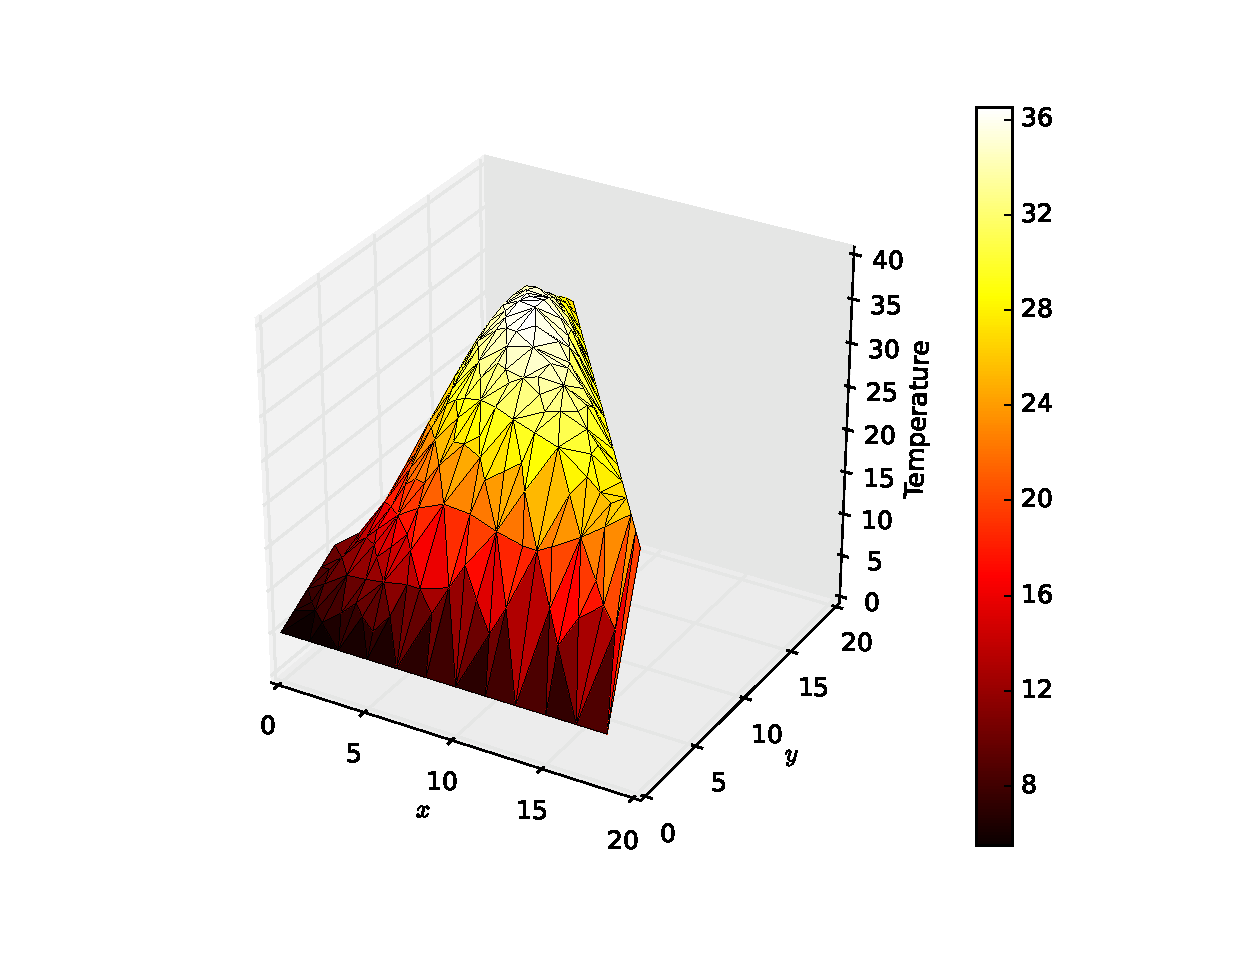
\includegraphics[width=\textwidth]{fig/exdam4_2.eps}
		\caption{}
		\label{fig:2}
	\end{subfigure}
	\begin{subfigure}[H]{0.33\textwidth}
		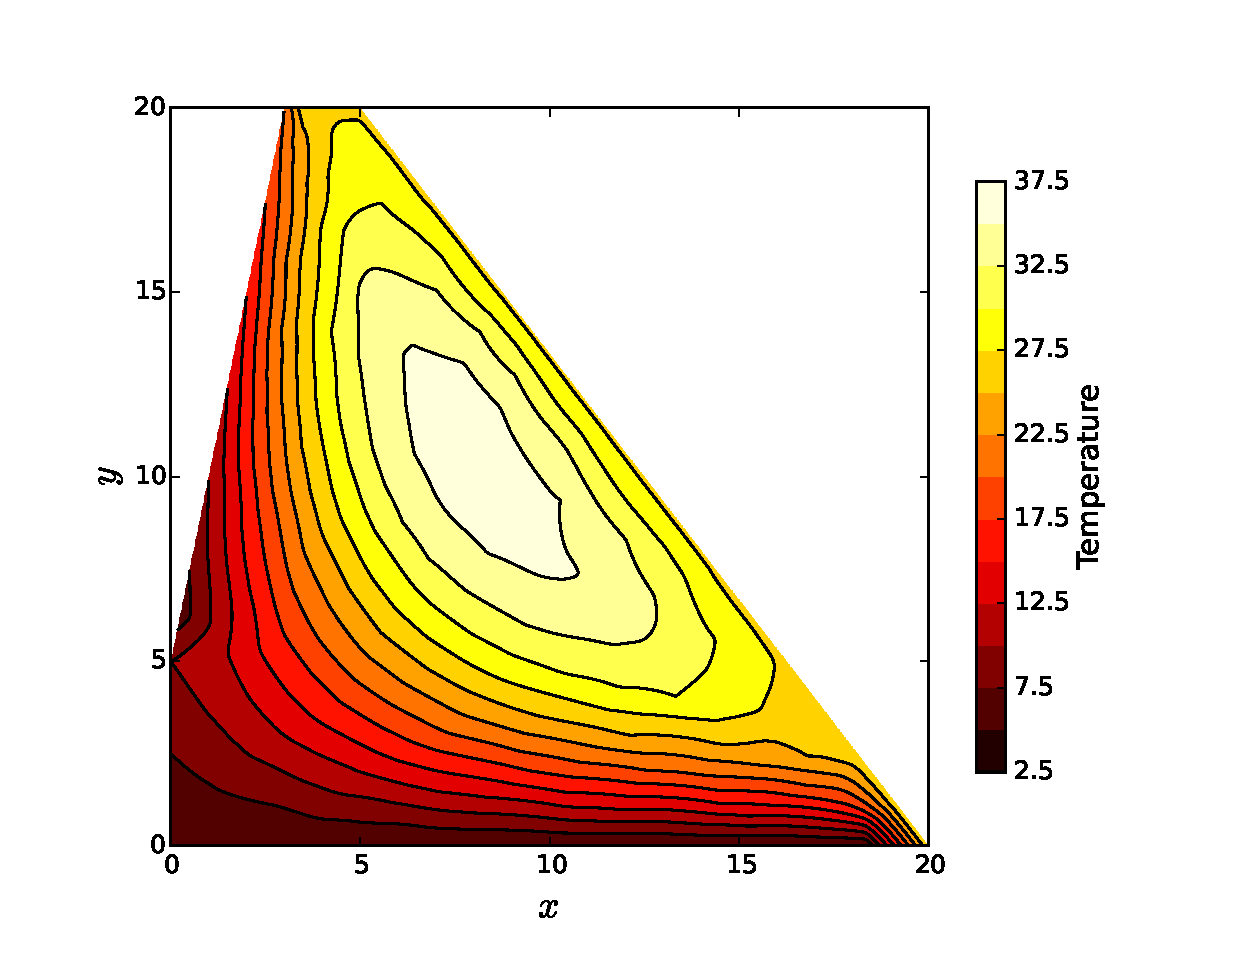
\includegraphics[width=\textwidth]{fig/exdam4_3.eps}
		\caption{}
		\label{fig:3}
	\end{subfigure}
	\caption{Internal load equals $q=x_1^2/10 + x_2^2/10$, temperature on the sides starts at the bottom and goes ccw $T=[5, 27, 27, x2, x2+5]$.}
	\label{fig:3_1}
\end{figure}


\subsection{General Tests}

\begin{figure}[H]
\centering
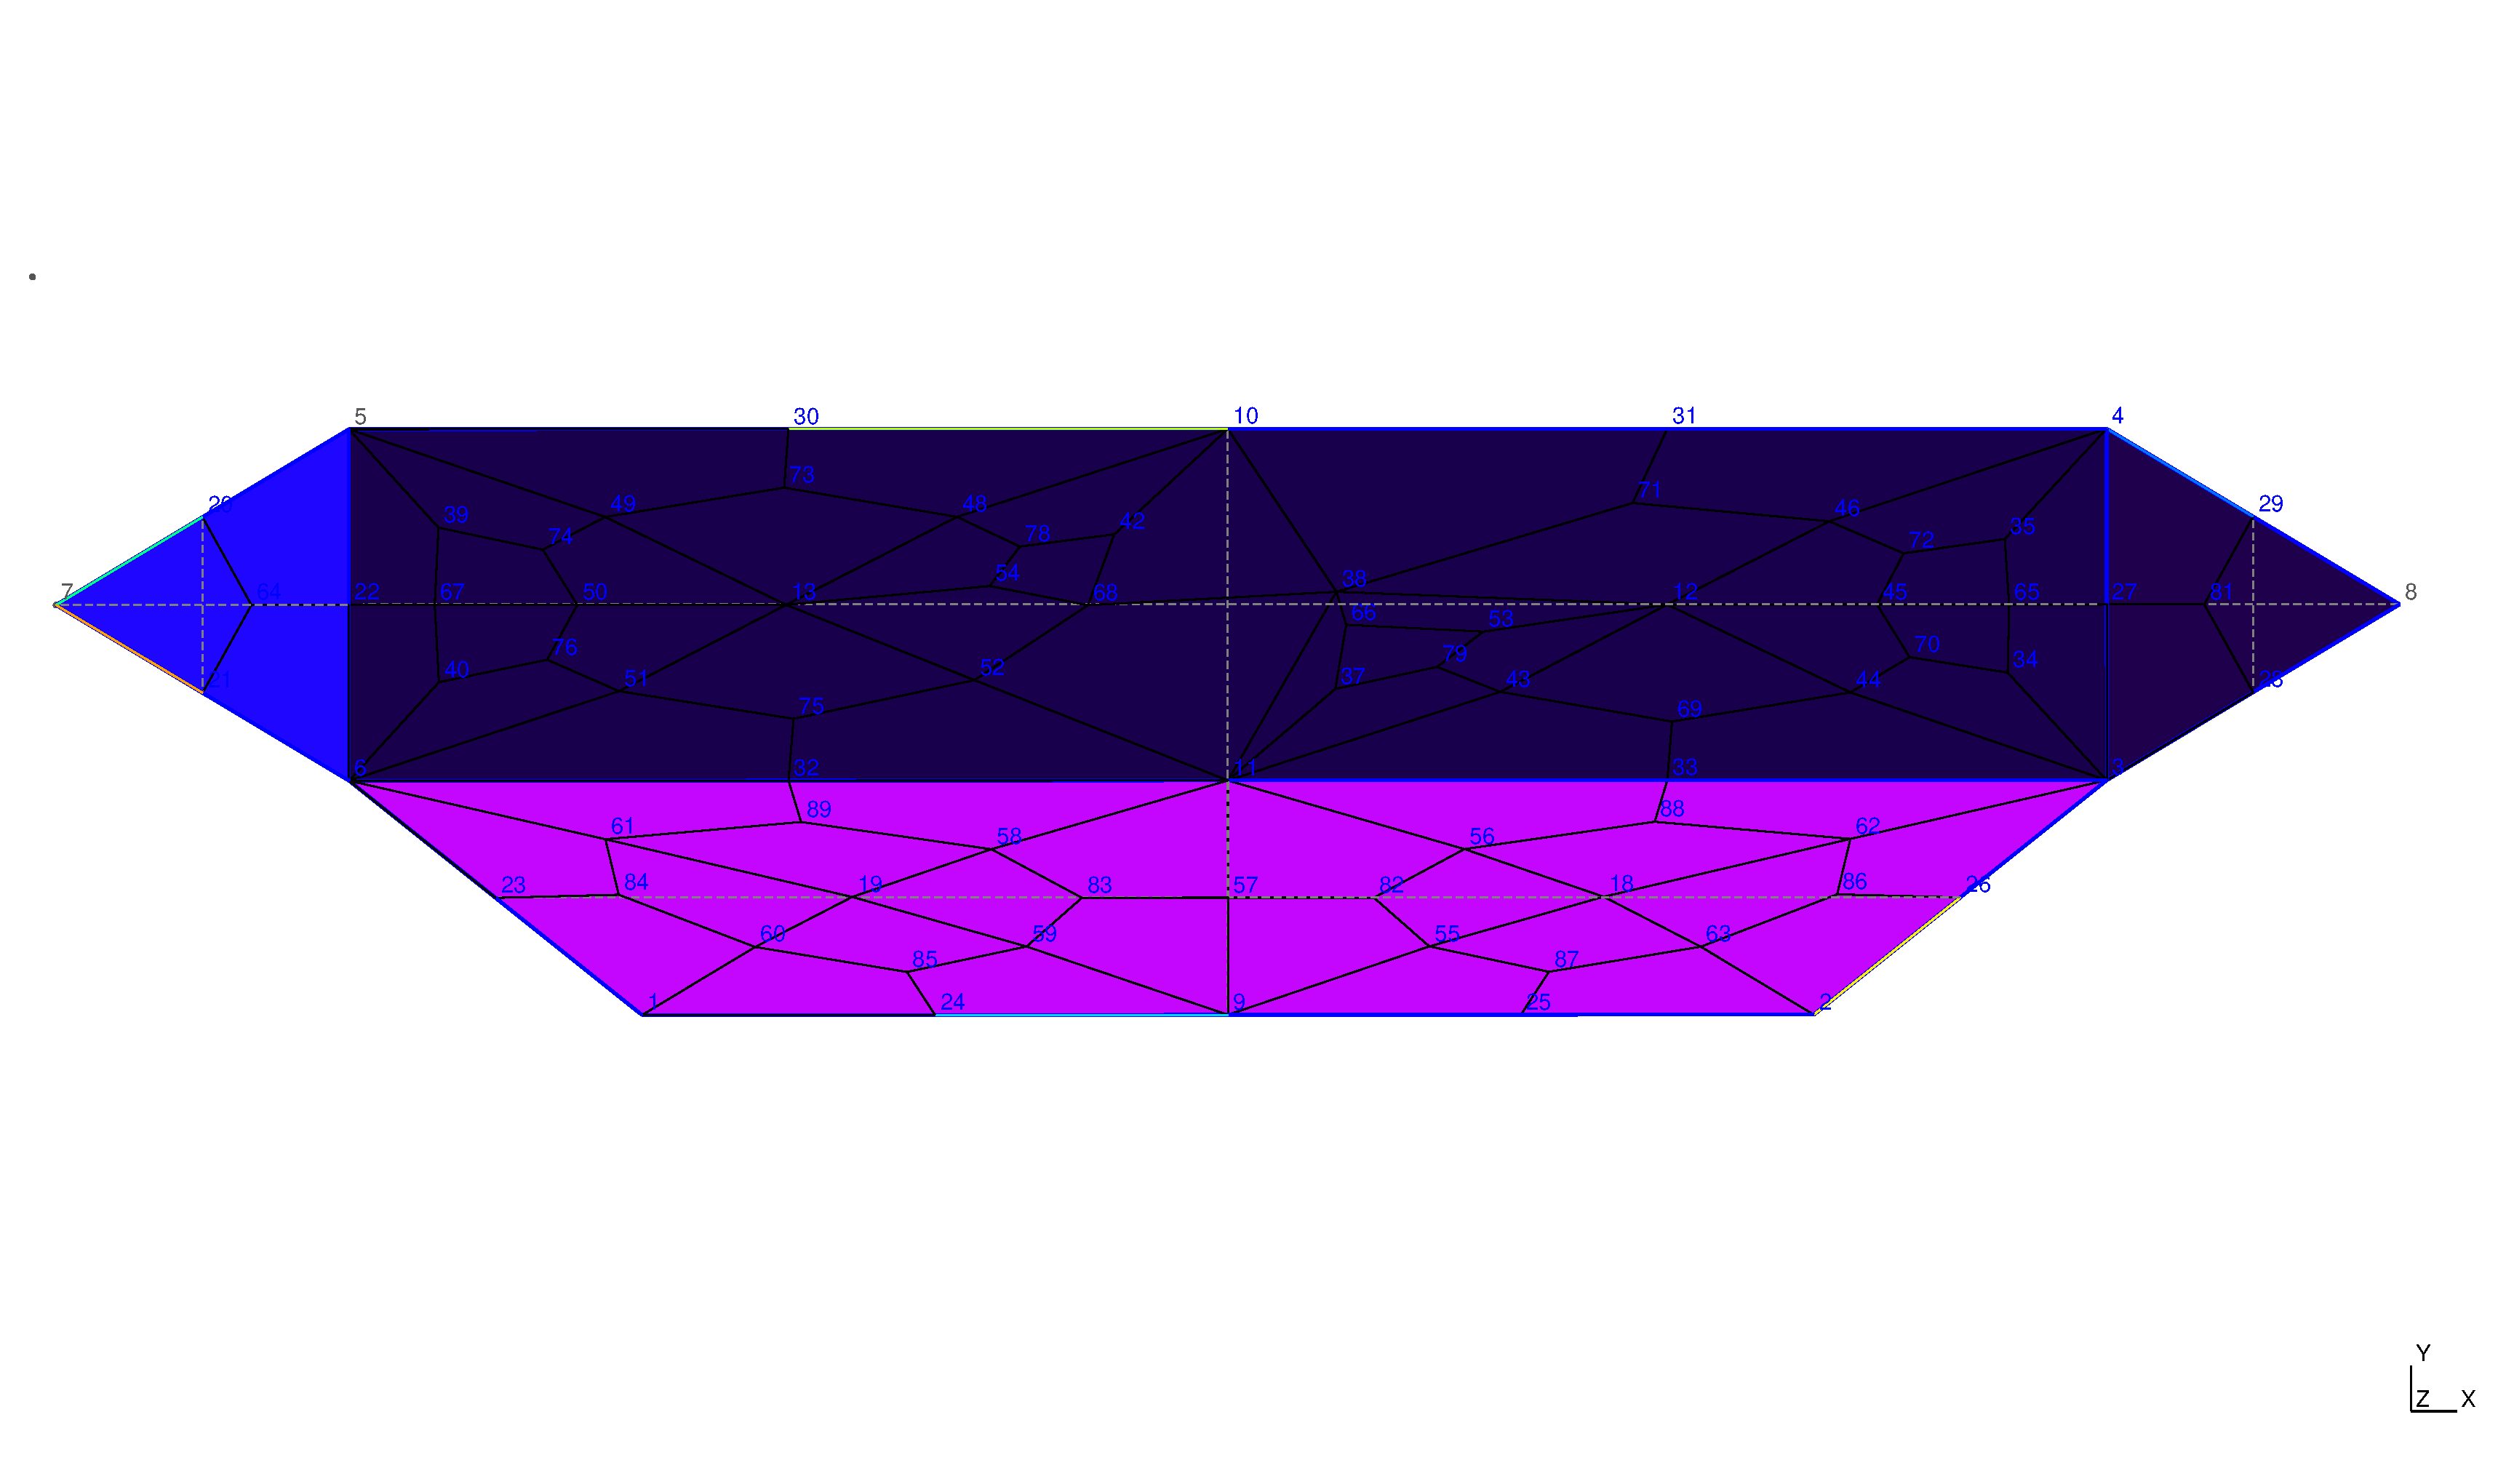
\includegraphics[width=.6\textwidth]{fig/test3_4.eps}
\caption{Modelon gmsh with different materials. The triangles have thermal diffusivity $k=5$, the center has $k=10$ and the bottom part $k=20$}
\end{figure}

\begin{figure}[H]
\centering
	\begin{subfigure}[H]{0.32\textwidth}
		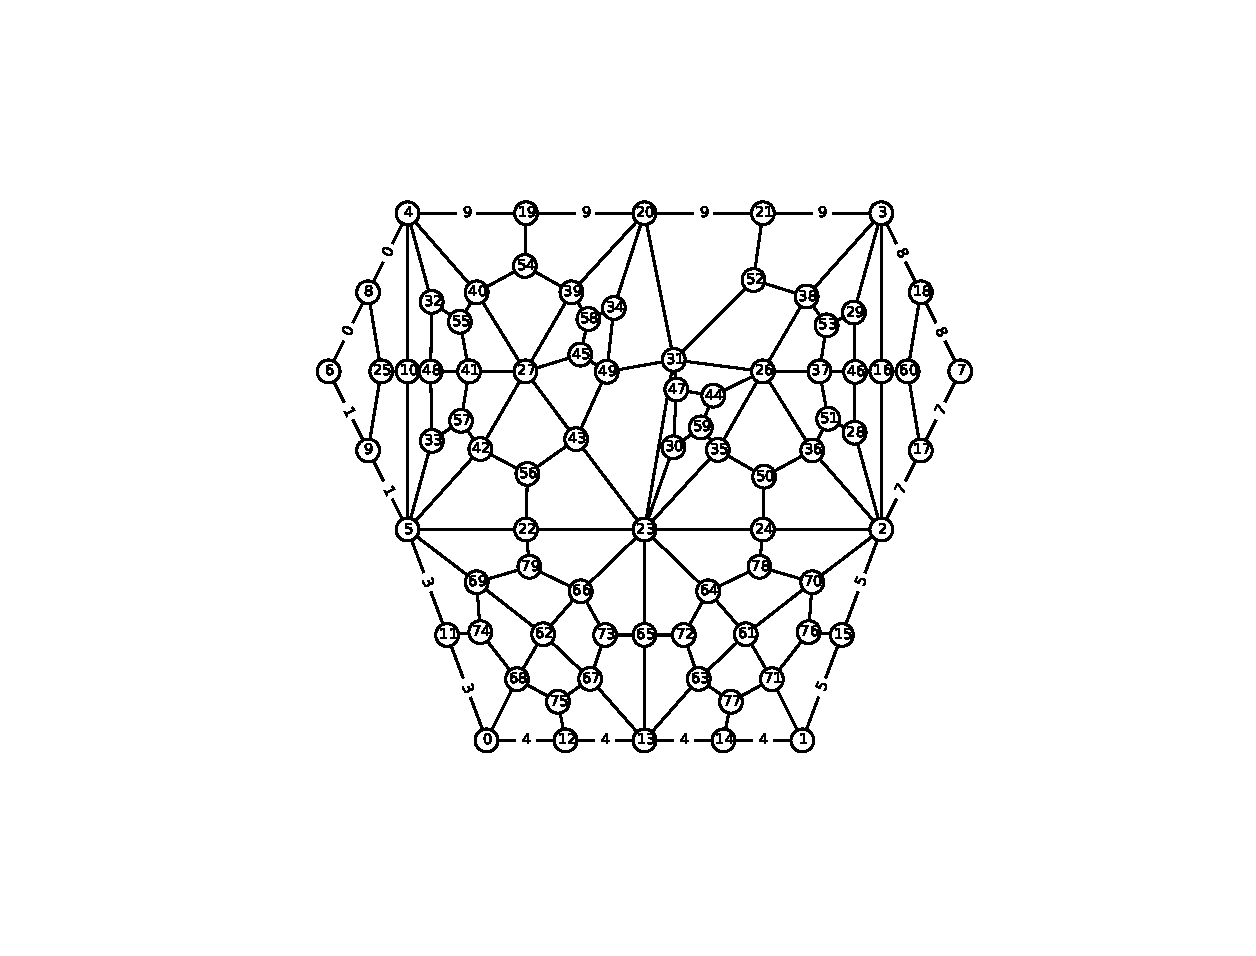
\includegraphics[width=1.3\textwidth]{fig/test3_1.eps}
		\caption{}
		\label{fig:1}
	\end{subfigure}
	\begin{subfigure}[H]{0.33\textwidth}
		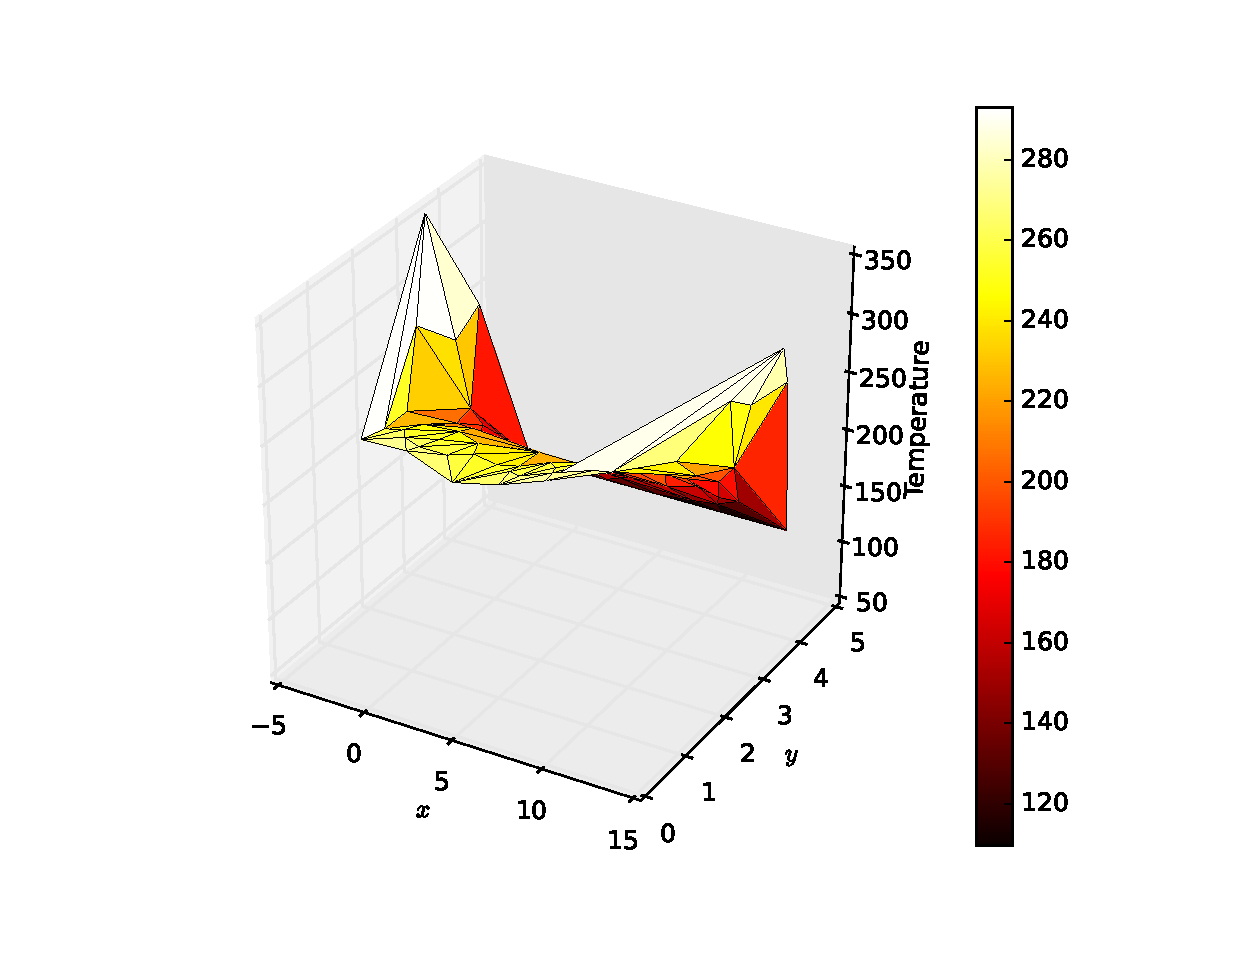
\includegraphics[width=\textwidth]{fig/test3_2.eps}
		\caption{}
		\label{fig:2}
	\end{subfigure}
	\begin{subfigure}[H]{0.33\textwidth}
		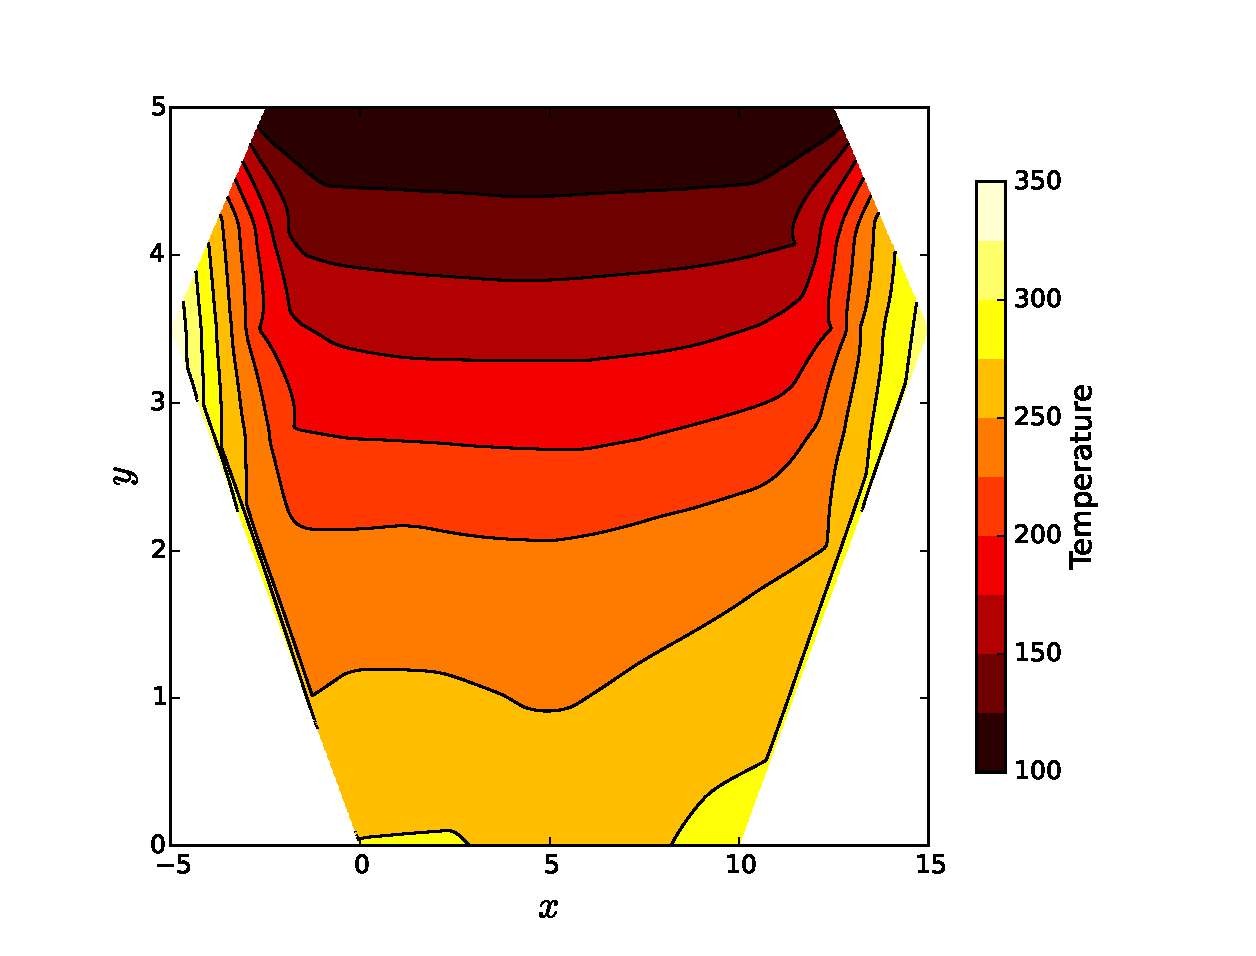
\includegraphics[width=\textwidth]{fig/test3_3.eps}
		\caption{}
		\label{fig:3}
	\end{subfigure}
	\caption{Internal load equals $q=0$, temperature on the sides $T=[9:100]$, flux on sides $t=[3:200, 0:100, 1:100, 4:300, 5:200, 7:100, 8:100]$. Number of elements equals 69.}
	\label{fig:3_1}
\end{figure}

\begin{figure}[H]
\centering
	\begin{subfigure}[H]{0.32\textwidth}
		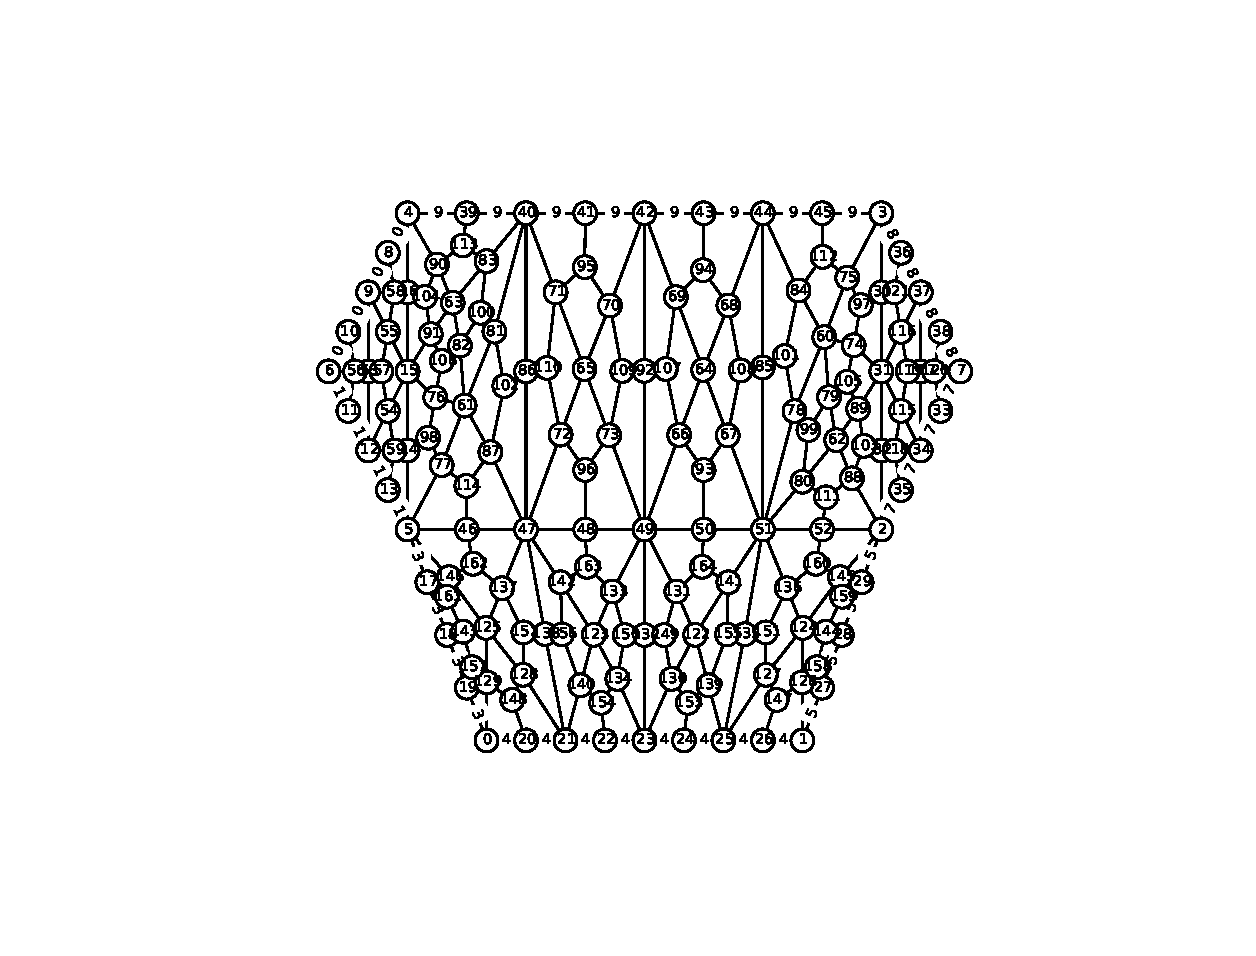
\includegraphics[width=1.3\textwidth]{fig/test4_1.eps}
		\caption{}
		\label{fig:1}
	\end{subfigure}
	\begin{subfigure}[H]{0.33\textwidth}
		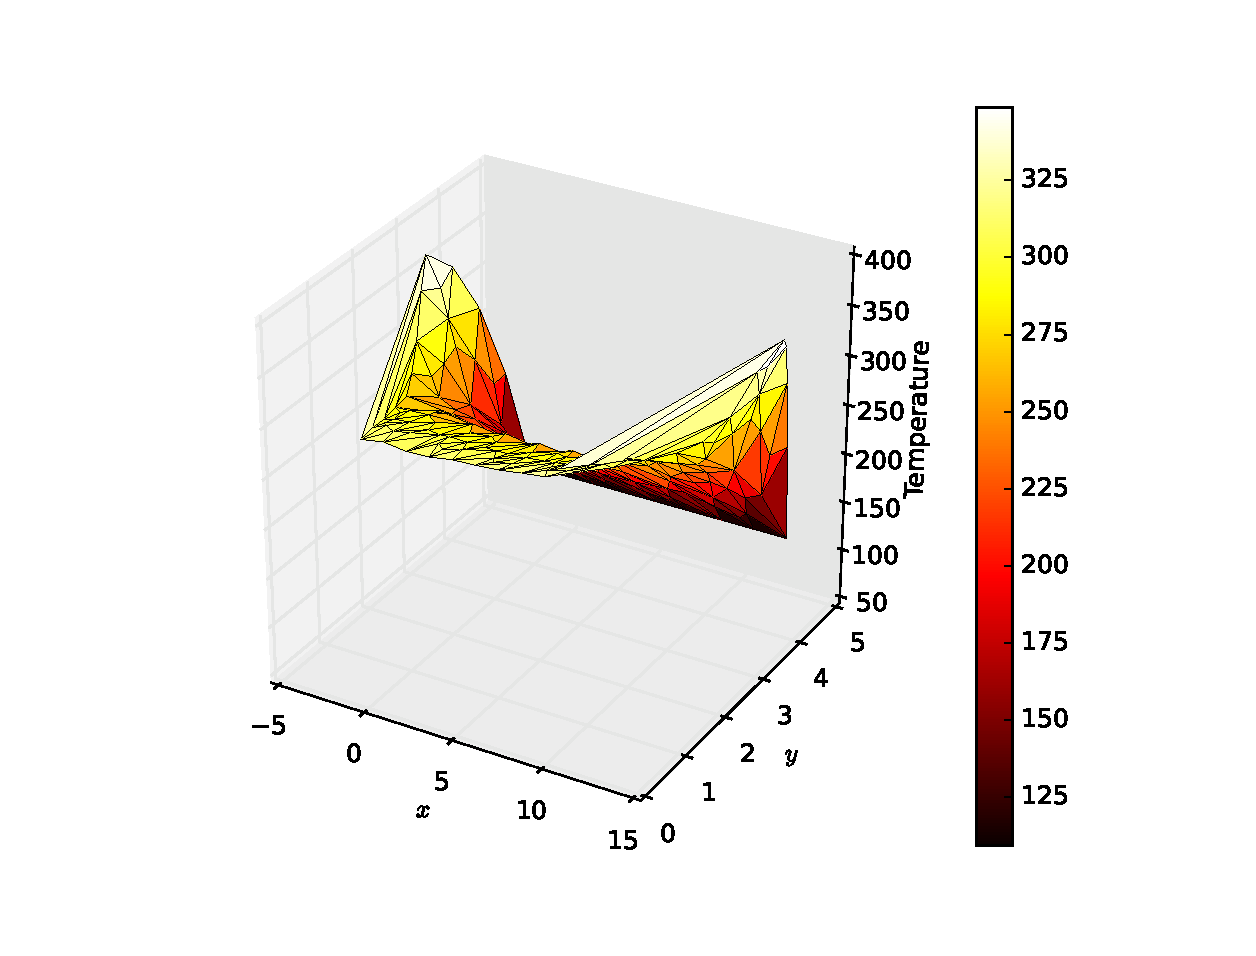
\includegraphics[width=\textwidth]{fig/test4_2.eps}
		\caption{}
		\label{fig:2}
	\end{subfigure}
	\begin{subfigure}[H]{0.33\textwidth}
		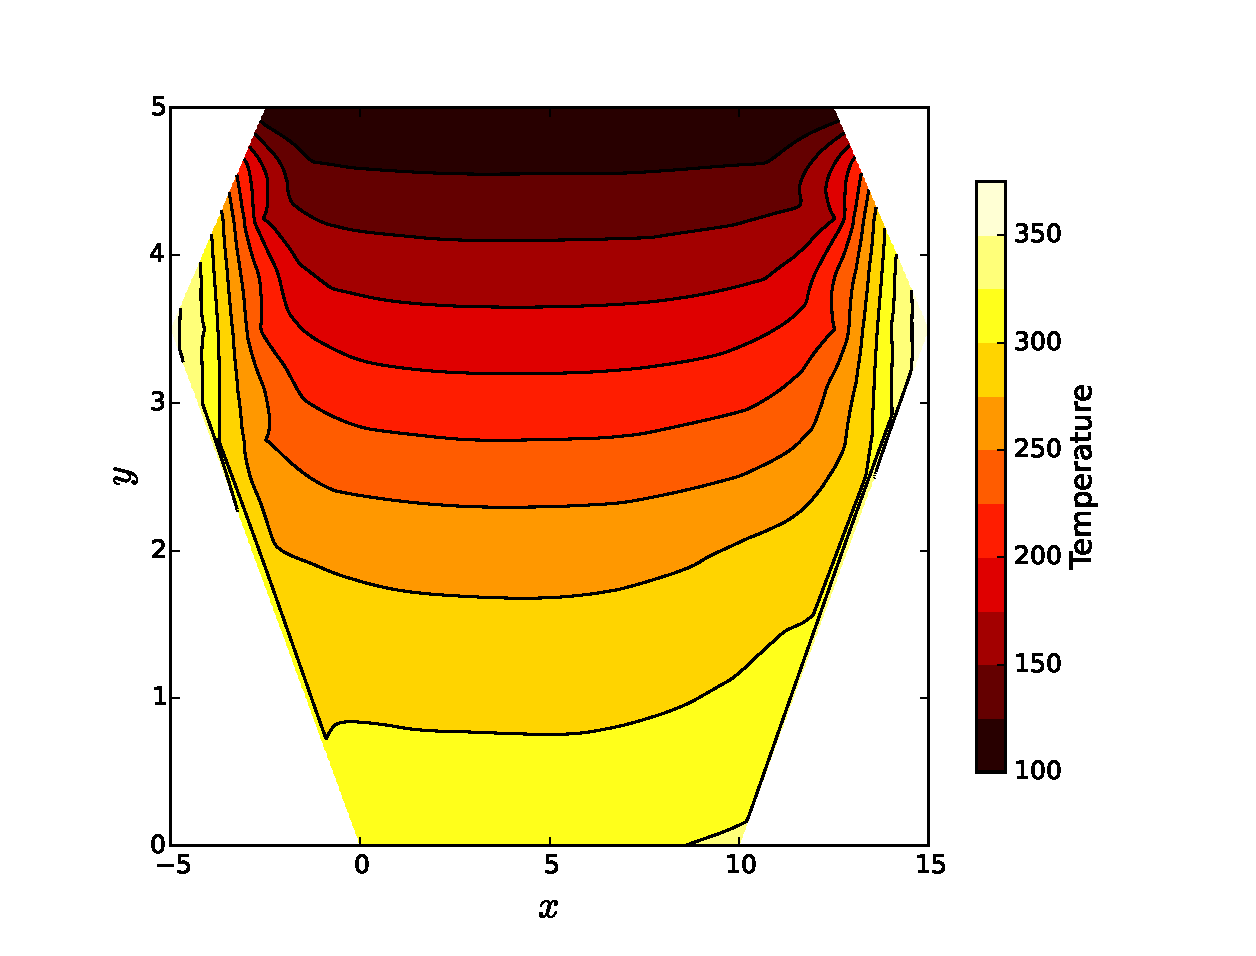
\includegraphics[width=\textwidth]{fig/test4_3.eps}
		\caption{}
		\label{fig:3}
	\end{subfigure}
	\caption{Internal load equals $q=0$, temperature on the sides $T=[9:100]$, flux on sides $t=[3:200, 0:100, 1:100, 4:300, 5:200, 7:100, 8:100]$. Number of elements equals 144.}
	\label{fig:3_1}
\end{figure}


\begin{figure}[H]
\centering
	\begin{subfigure}[H]{0.32\textwidth}
		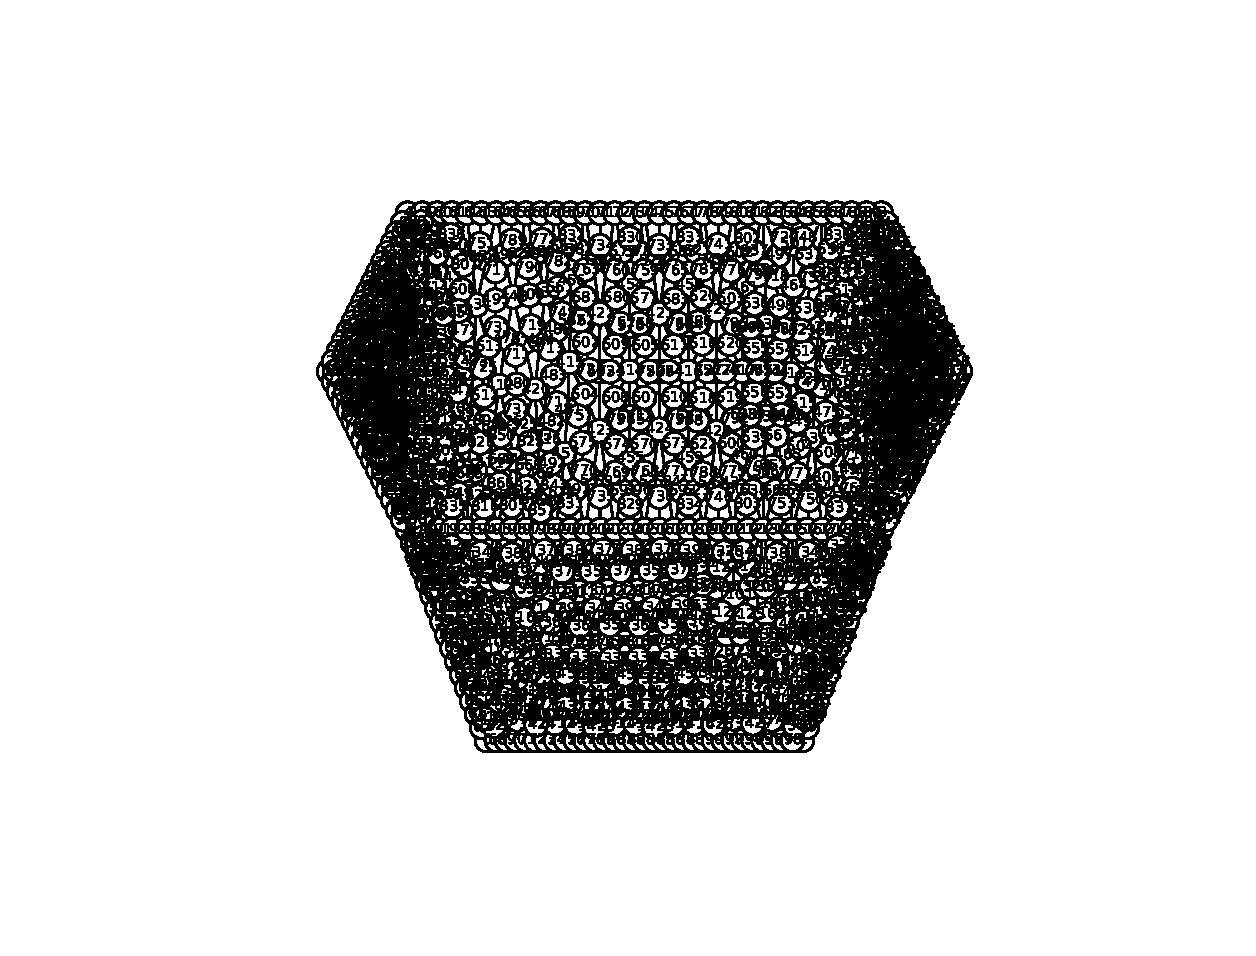
\includegraphics[width=1.3\textwidth]{fig/test5_1.eps}
		\caption{}
		\label{fig:1}
	\end{subfigure}
	\begin{subfigure}[H]{0.33\textwidth}
		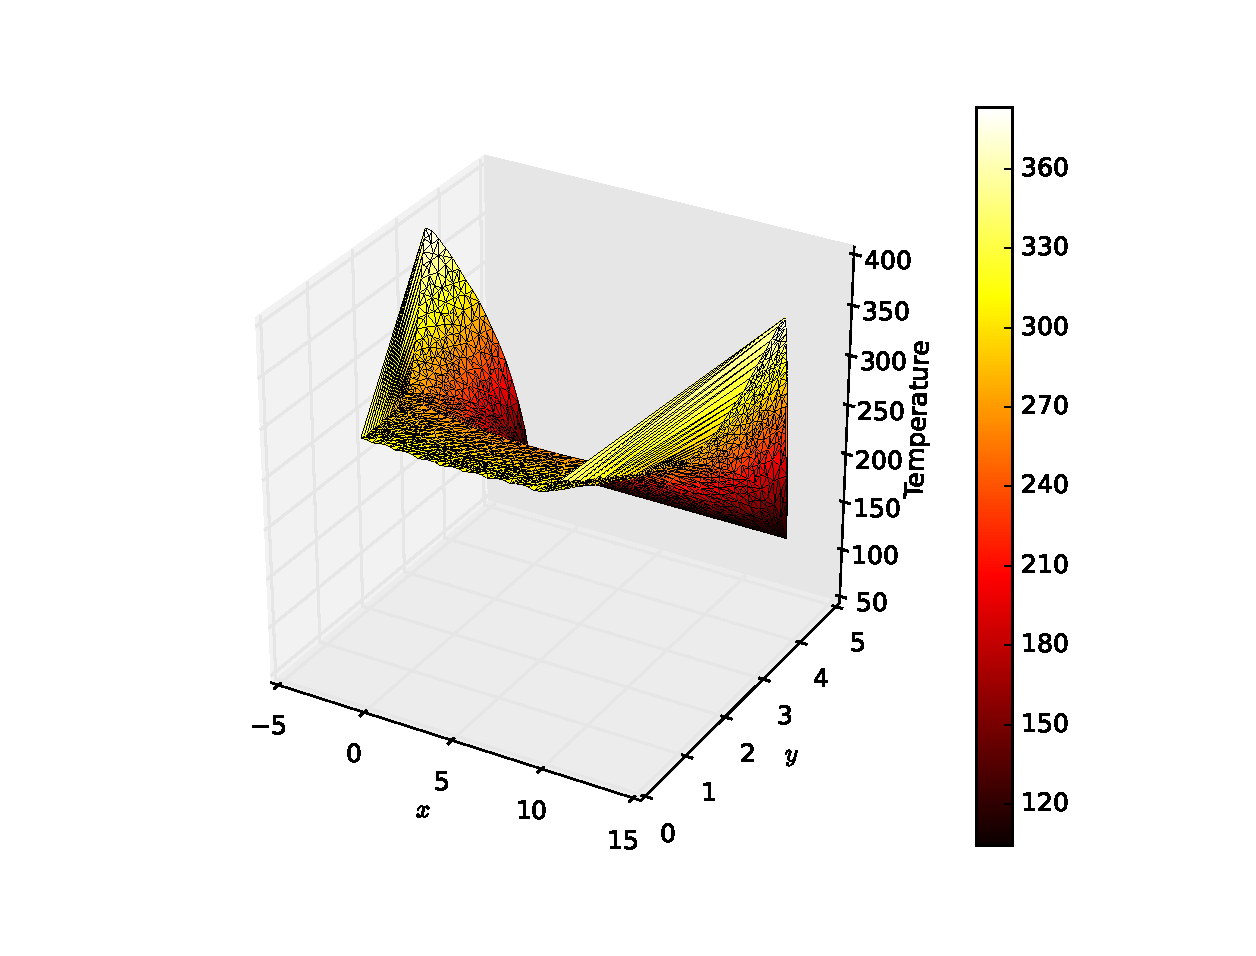
\includegraphics[width=\textwidth]{fig/test5_2.eps}
		\caption{}
		\label{fig:2}
	\end{subfigure}
	\begin{subfigure}[H]{0.33\textwidth}
		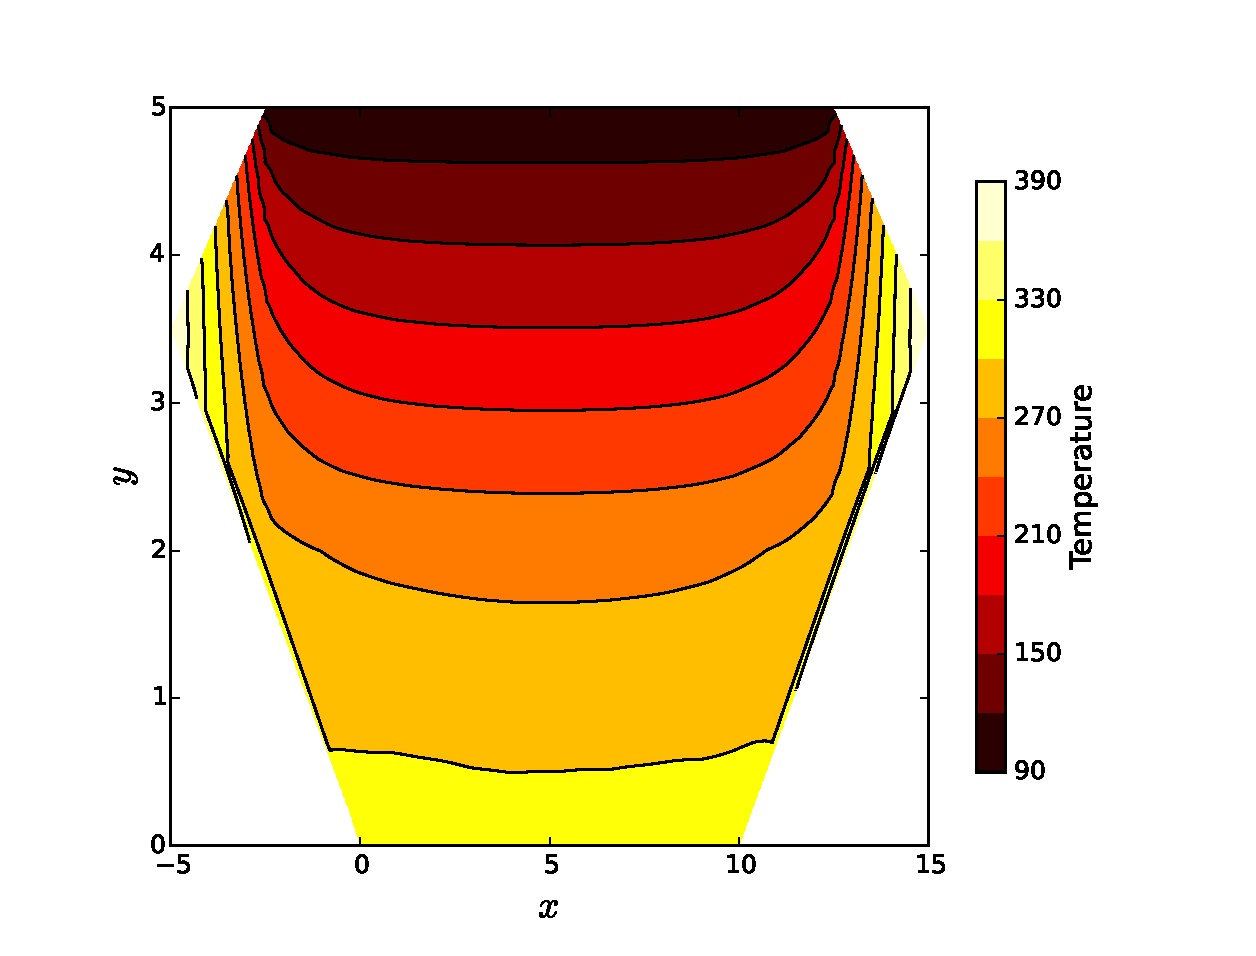
\includegraphics[width=\textwidth]{fig/test5_3.eps}
		\caption{}
		\label{fig:3}
	\end{subfigure}
	\caption{Internal load equals $q=0$, temperature on the sides $T=[9:100]$, flux on sides $t=[3:200, 0:100, 1:100, 4:300, 5:200, 7:100, 8:100]$. Number of elements equals 1386.}
	\label{fig:3_1}
\end{figure}

\subsection{Dam with non-convex Geometry}



\begin{figure}[H]
\centering
	\begin{subfigure}[H]{0.3\textwidth}
		\includegraphics[width=1.2\textwidth]{fig/exdam5_1.eps}
		\caption{}
		\label{fig:1}
	\end{subfigure}
	\begin{subfigure}[H]{0.33\textwidth}
		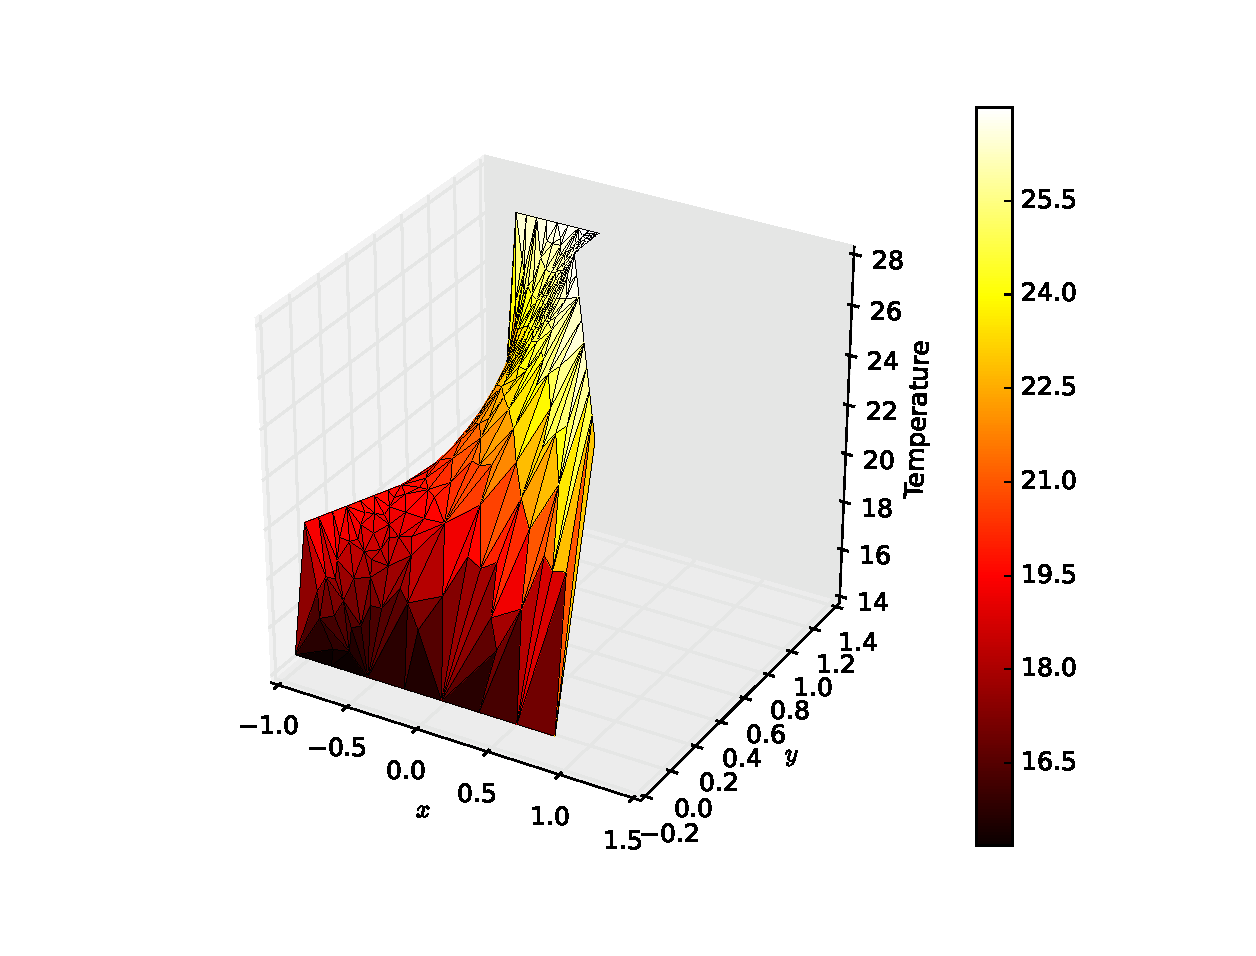
\includegraphics[width=\textwidth]{fig/exdam5_2.eps}
		\caption{}
		\label{fig:2}
	\end{subfigure}
	\begin{subfigure}[H]{0.33\textwidth}
		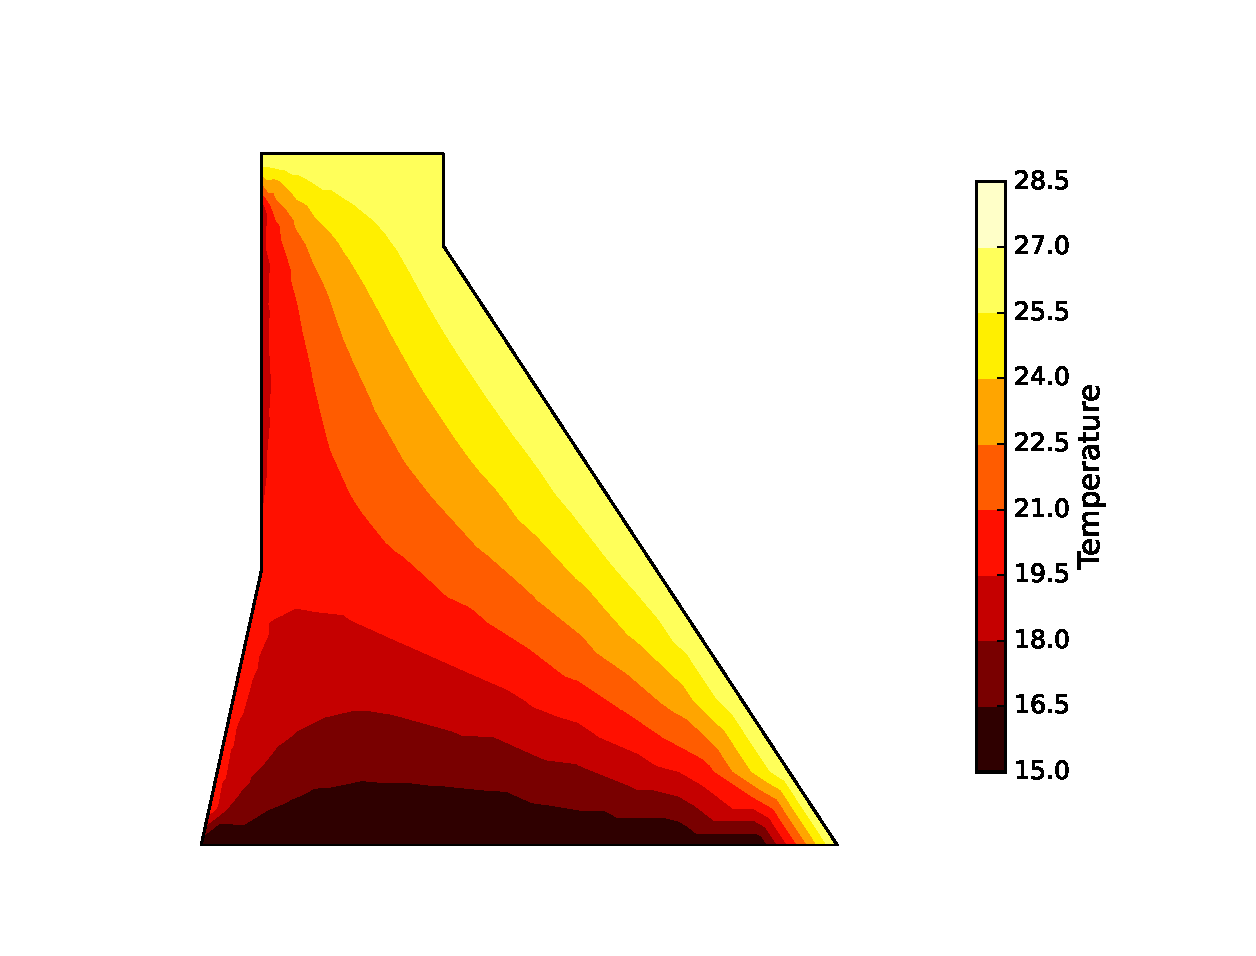
\includegraphics[width=\textwidth]{fig/exdam5_3.eps}
		\caption{}
		\label{fig:3}
	\end{subfigure}
	\caption{Internal energy source $q=0$, temperature assign on boundaries $T=\{0:20-x2, 1:20-x2, 2:15, 3:27, 4:27, 5:27\}$, no flux assigned.}
	\label{fig:3_1}
\end{figure}


\end{document}